\documentclass[10pt,polish,a4paper,oneside]{ppfcmthesis}

\usepackage[utf8]{inputenc}
\usepackage[OT4]{fontenc}



\usepackage[widespace]{fourier}   % Use Utopia font set
\usepackage[scaled=0.875]{helvet} % Use Helvetica for sans-serif
\renewcommand{\ttdefault}{lmtt}   % Use Lucida Mono for monotype
\usepackage{booktabs}             % Booktabs for tables
\usepackage{multirow}
\usepackage{algorithm2e}
\usepackage{placeins}
\usepackage{alltt}
\usepackage{amsmath}
\usepackage{caption}
\usepackage{subcaption}
\renewcommand{\listalgorithmcfname}{Lista algorytmów}
\renewcommand{\algorithmcfname}{Algorytm}

\newcommand{\SA}[1]{$\mathit{SA}_{#1}$}
\newcommand{\ISA}[1]{$\mathit{ISA}_{#1}$}
\DeclareMathAlphabet{\mathcal}{OMS}{cmsy}{m}{n}
\newcommand{\bigO}[0]{\mathcal{O}}
\newcommand{\dollar}[0]{\$}

\author{Jakub Lamprecht}

\title{Badawczy system rozpoznawania wykorzystujący obraz tęczówki oka}

\ppsupervisor{dr~inż.~Tomasz Piaścik}
\ppyear{2019}      % Year of final submission (not graduation!)

\begin{document}
% Front matter starts here
\frontmatter\pagestyle{empty}%
\maketitle\cleardoublepage%

% Blank info page for "karta dyplomowa"
\thispagestyle{empty}\vspace*{\fill}%
\begin{center}Tutaj przychodzi karta pracy dyplomowej;\\oryginał wstawiamy do wersji dla archiwum PP, w pozostałych kopiach wstawiamy ksero.\end{center}%
\vfill\cleardoublepage%

% Table of contents.
\pagenumbering{Roman}\pagestyle{ppfcmthesis}%
\tableofcontents* \cleardoublepage%

% Main content of your thesis starts here.
\mainmatter%
\chapter{Wprowadzenie}

% [DW] Cytowania normalnie, bez dodatkowych nawiasów; poprawiłem niektóre, zrób pozostałe.

Wraz ze zwiększeniem stopnia informatyzacji na świecie zwiększa się również iloś\'c przechowywanych przez
systemy informatyczne danych, w tym również tych poufnych, do których dostęp powinny mie\'c tylko
określone osoby. W związku z tym zapotrzebowanie na systemy weryfikacji i identyfikacji rośnie. Metody
uwierzytelniania można podzieli\'c ze względu na element użyty do przeprowadzenia procesu:

\begin{itemize}
  \item metody wykorzystujące informacje, do których dostęp mają wyłącznie osoby uprawnione (np. hasło, pin),
  \item metody wykorzystujące przedmiot w którego posiadaniu są jedynie osoby uprawnione,
  \item metody wykorzystujące cechy fizyczne osób uprawnionych.
\end{itemize}

Z wymienionych metod najbezpieczniejszymi są te ostatnie, inaczej zwane metodami biometrycznymi.
Twórcy systemów wykorzystujących te metody poszukują cech fizycznych człowieka, które pozwalają na
nieinwazyjne, odporne na oszustwa uwierzytelnienie. Jedną z najbardziej obiecujących cech
w świecie biometrii jest tęczówka, której rozpoznawanie jest przedmiotem niniejszej pracy. Mimo, że
tęczówka nie jest cechą idealną ze względu na przykładowo koszty wdrożenia takiego systemu,
to systemy wykorzystujące tę cechę biometryczną charakteryzują się niskim współczynnikiem nieprawidłowej
identyfikacji.

\section{Cel i~zakres pracy}

Celem tej pracy było zaprojektowanie i stworzenie aplikacji pozwalającej na przeprowadzenie procesu
rozpoznawania tęczówki oka oraz przegląd literatury i implementacja algorytmów normalizacji,
enkodowania oraz dopasowania tęczówki. Jednym z wymagań dla tworzonego programu było, aby działał
on w dwóch trybach:

\begin{itemize}
    \item Krokowym - tryb umożliwiający użytkownikowi stopniowe przejście przez proces rozpoznawania
    z możliwością wyboru metod oraz parametrów dla poszczególnych kroków, a także podglądu wyników dla
    każdego z nich.

    \item Wsadowym - tryb umożliwiający automatyczne przeprowadzenie procesu rozpoznawania opisanego przez
    plik konfiguracyjny wygenerowany w trybie krokowym dla większego zbioru obrazów.
\end{itemize}

\noindent
Ważnym aspektem dla tworzonej aplikacji była również użyteczność i przyjazność interfejsu użytkownika,
który miał zachęcać do korzystania z aplikacji.

\section{Struktura pracy}

Struktura pracy jest następująca. Rozdział drugi poświęcony został wstępowi do zagadnienia
rozpoznawania tęczówki. Zawiera on ogólne informacje o historii, anatomii oka i jego właściowościom
biometrycznym oraz zastosowaniom biometrycznym tęczówki. Traktuje on również ogólnie o procesie
przetwarzania obrazu tęczówki. W kolejnym rozdziale opisane zostały technologie użyte w celu stworzenia
aplikacji, a także opis jej działania i funkcjonalności. Rodział czwarty jest w całości poświęcony
algorytmom normalizacji, kodowania oraz dopasowania i zasadzie ich działania. Piąty Rozdział
przedstawia informacje na temat eksperymentu przeprowadzonego z wykorzystaniem wytworzonej
aplikacji i jego wyników. Rozdział szósty stanowi podsumowanie pracy i wskazuje potencjalne
kierunki dalszego jej rozwoju.


\chapter{Podstawy teoretyczne}

Pierwsza wzmianka o użyciu tęczówki w celu identyfikacji jednostki datowana jest na rok
1936, a autorem jej był okulista Frank Burch \cite{FBIGov}. W roku 1985 okuliści Leonard Flom oraz
Aran Safir przedstawili tezę popartą badaniami klinicznymi, że w świecie nie istnieją dwie
identyczne tęczówki, a w roku 1987 opatentowali pomysł Bruch'a. Nie byli oni jednak w
stanie stworzy\'c systemu i algorytmów pozwalających na identyfikację osoby na podstawie
obrazu tęczówki. W roku 1989, na ich prośbę, matematyk John Daugman stworzył algorytmy
pozwalające na automatyczną identyfikację tęczówki, które następnie opatentował w roku 1994.
\cite{Misztal2012}
Algorytmy te są podwaliną większości rozwiąza\'n zastosowanych w systemach wykorzystujących
obraz tęczówki oka. W dalszej części tego rozdziału przedstawione zostaną informacje teoretyczne
pozwalające na zrozumienie jaką rolę odgrywa rozpoznawanie tęczówki w systemach biometrycznych.

\section{Budowa tęczówki}

\begin{figure}[ht]
  \centering
  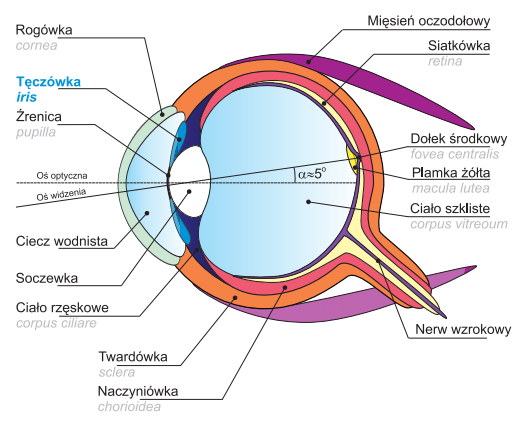
\includegraphics[width=0.7\textwidth]{images/intro/eyeStructure.png}
  \caption{Schemat anatomiczny oka ludzkiego \cite{Czajka}.}
  \label{fig:eyeStructure}
\end{figure}

Tęczówka jest umięśnioną częścią błony naczyniowej, która otacza otwór zwany \'zrenicą.
Jej częś\'c obwodowa przechodzi w ciało rzęskowe utrzymujące soczewkę \cite{Czajka}. Z zewnątrz
otoczona jest prze\'zroczystą rogówką pełniącą funkcję ochronną. Głównym zadaniem tęczówki
jest kontrolowanie strumienia światła dostającego się przez \'zrenicę do oka przez kurczenie i
rozkurczanie swoich mięśni. Bierze ona również udział w procesie akomodacji oka odpowiedzialnym
za ostre widzenie. Dzięki zawartemu w jej komórkach barwnikowi - \textit{melaninie}, może ona przyjmowa\'c różne kolory.
Kolor tęczówki najcześciej jest pomijany w procesie rozpoznawania ze względu na liczne możliwości
jego zaburzenia przykładowo w wyniku chorób, lub zmian hormonalnych regulujących stężenie melaniny.

Patrząc na obraz tęczówki (rysunek \ref{fig:irisExample}) możemy dostrzec jej charakterystyczną teksturę. Wynika ona z ułożenia
beleczek i zatok na jej powierzchni. Tęczówka kształtuje się od trzeciego do ósmego miesiąca życia
płodu i po tym procesie pozostaje niezmienna do końca życia (zakładając brak chorób).
W wyniku zgonu ulega zniszczeniu w ciągu pięciu sekund.

\begin{figure}[ht]
  \centering
  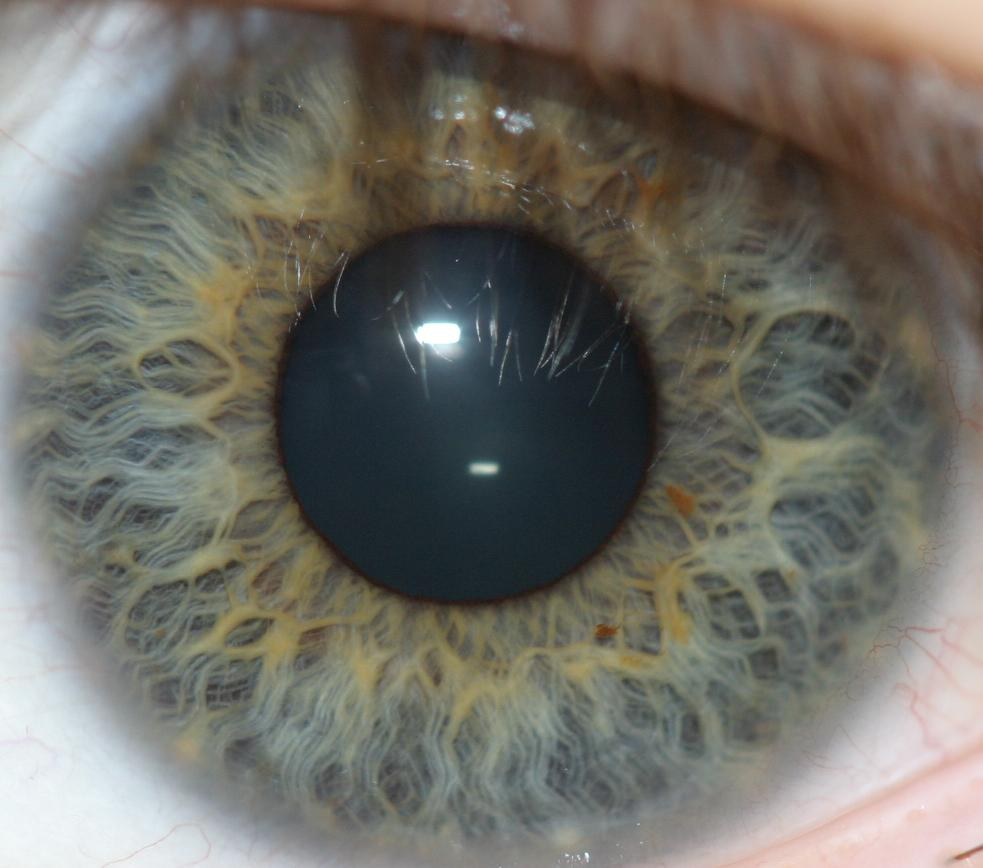
\includegraphics[width=0.5\textwidth]{images/intro/irisExample.png}
  \caption{Przykładowy obraz tęczówki oka.}
  \label{fig:irisExample}
\end{figure}

\section{Tęczówka w biomterii}

Aby cechy fizyczne były użyteczne z punktu widzenia biometrii powinny spełnia\'c następujące
wymagania:

\begin{itemize}
  \item uniwersalnoś\'c - każdy człowiek powinien posiada\'c daną cechę,
  \item unikalno\'c - cecha powinna by\'c unikalna dla każdej osoby,
  \item mierzalnoś\'c - łatwoś\'c pobrania informacji,
  \item trwałoś\'c i niezmiennoś\'c - cecha powinna by\'c niezmienna w trakcie życia,
  \item szybkoś\'c i skutecznoś\'c działania systemu opartego o cechę,
  \item akceptowalnoś\'c społeczna,
  \item możliwoś\'c oszukania systemu.
\end{itemize}

Tęczówka spełnia powyższe wymagania w stopniu bardzo dobrym. Większoś\'c populacji posiada
ją. Badania wykazują, że jest ona unikalna dla każdego człowieka, nawet dla bli\'zniąt jednojajowych.
Co więcej, tęczówki oka lewgo i prawego u jednego człowieka również różnią się między sobą. Tęczówka zawiera
wiele punktów charakterystycznych i detali, dzięki czemu rośnie skutecznoś\'c systemu opartego na jej obrazie.
Tak jak wcześniej zostało to wspomniane, tęczówka kształtuje się na etapie płodu i pozostaje niezmienna
przez resztę życia. Dzięki rozszerzaniu i kurczeniu się w celu kontrolowania przepływu światła w zależności
od oświetlenia otoczenia, oszukanie systemu przez zdjęcie jest mocno utrudnione. Dodatkowym atutem
jest fakt, że tęczówka jest dobrze chronionym, a jednocześnie dobrze widocznym organem, co ułatwia
pobranie obrazu.

Poniżej wymienione zostały wady tęczówki jako cechy biometrycznej:

\begin{itemize}
  \item jest stosunkowo mała, co znacznie zmniejsza dystans z jakiego można pobra\'c o niej informacje
  \item znajduje się za wilgotną, zakrzywioną i odbijającą światło powierzchnią, co może potencjalnie
  wprowadza\'c zakłócenia w pobieranym obrazie
  \item jest umiejscowiona na ruchomej gałce ocznej, która umiejscowiona jest na ruchomej głowie, co może
  wprowadza\'c liczne niespójności rotacji między obrazami tej samej tęczówki
  \item częściowo zasłonięta przez powieki oraz rzęsy
\end{itemize}

Na rysunku poniżej (\ref{fig:irisBiometricsComparison}) przedstawione zostało porównanie tęczówki
z innymi cechami biometrycznymi w ramach wyżej wymienionych wymagań:

\begin{figure}[ht]
  \centering
  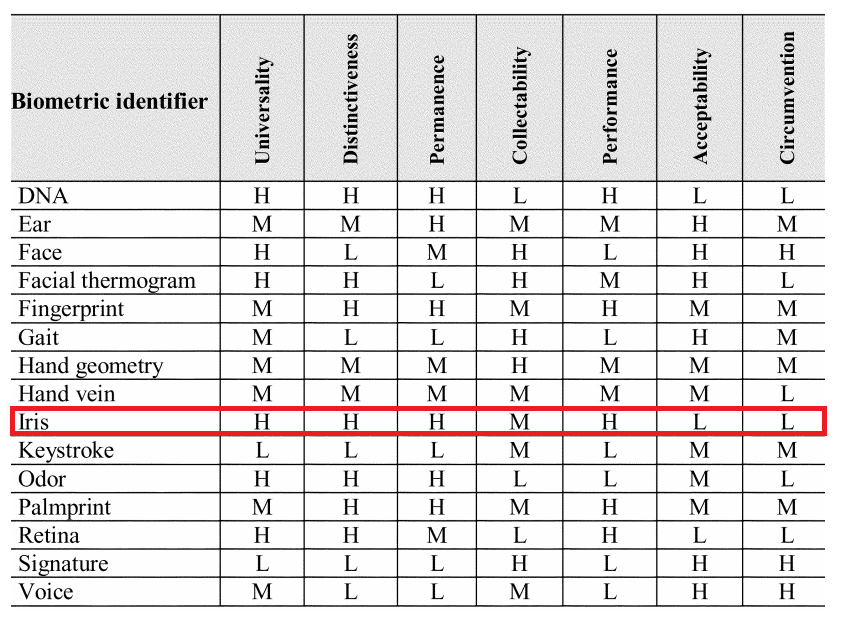
\includegraphics[width=0.8\textwidth]{images/intro/biometricsProperties.png}
  \caption{Porównanie cech biometrycznych \cite{IntroToBiometricRecognition}. Legenda: H - spełnione w wysokim
  stopniu, M - spełnione w średnim stopniu, L - spełnione w niskim stopniu.}
  \label{fig:irisBiometricsComparison}
\end{figure}

\section{Opis procesu rozpoznawania}

\noindent
Proces rozpoznawania tęczówki (rysunek \ref{fig:processDiagram}) można rozbi\'c na kilka etapów:

\begin{itemize}
  \item pobranie obrazu tęczówki,
  \item segmentacja,
  \item normalizacja,
  \item detekcja cech charakterystycznych
  \item dopasowanie
\end{itemize}

\begin{figure}[ht]
  \centering
  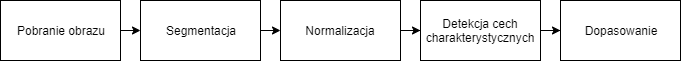
\includegraphics[width=0.8\textwidth]{images/intro/processDiagram.png}
  \caption{Diagram przedstawiający przebieg procesu rozpoznawania tęczówki}
  \label{fig:processDiagram}
\end{figure}

Pobranie obrazu tęczówki może wydawa\'c się stosunkowo proste, jednak zdecydowanie takie nie
jest. Zdjęcia tęczówki wykonywane w świetle widzialnym dają dobre wyniki dla tęczówek o jasnych
kolorach, natomiast podejście to może zawieś\'c w przypadku ciemnych kolorów tęczówek ze względu
na niski kontrast zdjęcia, co może prowadzi\'c do zlania się \'zrenicy i tęczówki w jedną całoś\'c.
Uniemożliwiłoby to wyodrębnienie tych dwóch elementów w etapie segmentacji.

Pobieranie obrazu w świetle widocznym może również prowadzi\'c do zmian szerokości tęczówki w trakcie
pobierania zdję\'c (różnica w oświetleniu między przetwarzaniem tęczówki w celu zapisania użytkownika
do bazy danych, a w momencie weryfikacji tożsamości), co może negatywnie wpływa\'c na działanie
systemu. Dodatkową wadą takiego podejścia jest występowanie w obrazie odbi\'c światła.

W celu wyeliminowania powyższych problemów zdjęcia tęczówki można wykonywa\'c w bliskiej podczerwieni \cite{IrisRecognitionPresentation},
dzięki czemu uzyskane obrazy nie posiadają zakłóceń w postaci odbi\'c światła, a także
zapewniają widocznoś\'c struktury tęczówki zarówno dla tych o jasnych, jak i ciemnych kolorach (rysunek \ref{fig:irisAcquisitionExample}).

\begin{figure}[ht]
  \centering
  \begin{subfigure}[b]{0.4\textwidth}
    \centering
    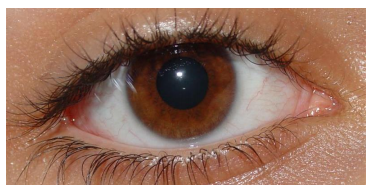
\includegraphics[width=\textwidth]{images/intro/eyeDaylight.png}
    \caption{Obraz tęczówki w świetle widzialnym}
  \end{subfigure}
  \begin{subfigure}[b]{0.4\textwidth}
    \centering
    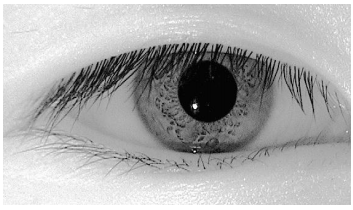
\includegraphics[width=\textwidth]{images/intro/eyeInfraRed.png}
    \caption{Obraz tęczówki w bliskiej podczerwieni}
  \end{subfigure}
  \caption{Róznice w pobieraniu obrazu tęczówki \cite{IrisRecognitionPresentation}.}
  \label{fig:irisAcquisitionExample}
\end{figure}


Następnym etapem jest proces segmentacji, w wyniku którego określane są parametry okręgów
tęczówki oraz \'zrenicy takie jak ich punkty środkowe oraz promienie. Często w ramach segmentacji
wykonywane jest również poszukiwanie powiek oraz innych zakłóceń na obrazie np. rzęs o których informacje
zapisywane są w masce zakłóceń określającej które fragmenty obrazu są znaczące dla procesu rozpoznawania,
a które nie. Algorytmy te działają w większości w oparciu o metody wykrywania krawędzi.
Metody segmentacji nie są przedmiotem niniejszej pracy i nie zostały w niej opisane.\newline

Znając parametry \'zrenicy oraz tęczówki możliwe jest wyodrębnienie z obrazu tylko i wyłącznie
punktów należących do tęczówki i zignorowanie reszty punktów obrazu. Wiedząc które piksele obrazu
reprezentują tęczówkę, możliwe jest przejście do kolejnego etapu, czyli ekstrakcji cech charakterystycznych
opisujących daną tęczówkę i zakodowania tych informacji w pewnej postaci. Posta\'c ta powinna umożliwia\'c
porównanie dwóch reprezentacji tęczówek i podjęcie decyzji o dopasowaniu bąd\'z niedopasowaniu.

Tak jak wcześniej zostało wspomniane, pierwszym, pionierskim systemem rozpoznawania tęczówki był
system opracowany przez Johna Daugmana \cite{DaugmanHowIrisRecognitionWorks}. Nie jest to jednak
jedyna praca traktująca o rozpoznawaniu tęczówki. W swoich pracach alternatywne rozwiązania
zaproponowali również Wildes \cite{Wildes} oraz Boles \cite{Boles}. W następnym rozdziale opisane
zostały algorytmy autorstwa Daugmana oraz ich implementacje.

\section{Zastosowania}

Ze względu na dokładnoś\'c działania i koszty związane z wprowadzeniem tego typu systemu
biometrycznego, zastosowania rozpoznawania tęczówki można znale\'z\'c głównie w systemach
wymagających największego stopnia bezpieczeństwa.

Jednym z sektorów w którym rozpoznawanie tęczówki znajduje miejsce jest bankowoś\'c. Banki
przechowują wiele tajnych informacji, które przedstawiane są osobom tylko i wyłącznie
po wcześniejszej weryfikacji tożsamości. Potencjalne naruszenia bezpieczeństwa mogłyby doprowadzi\'c
do wycieku danych osobowych czy nawet kradzieży.

Rozpoznawanie tęczówki znajduje również zastosowanie w sektorze zdrowia. Pozwala ono na dokładną
identyfikację osoby i ustalenie statusu ubezpieczenia, a także prostsze odnalezienie kartoteki
medycznej. Znalazły one zastosowanie w szpitalach w całym świecie w celu rozwiązania problemu z
kradzieżami noworodków. Dostęp do sali w której znajduje się dziecko posiadają jedynie doktorzy,
pielęgniarki oraz matka dziecka.

Jednym z największych sektorów w których stosowane jest rozpoznawanie tęczówki jest kontrola graniczna
oraz imigracyjna. W wielu krajach postanowiono uży\'c wzoru tęczówki przechowywanego w systemie jako głównego
zabezpieczenia przed nielegalnym przekroczeniem granicy. Rozwiązania takie zostały zaimplementowane na lotniskach
w Stanach Zdjednoczonych, Kanadzie, Wielkiej Brytanii czy Holandii.

Jednym z największych zastosowań jest projekt Aadhaar w Indiach, którego celem było wprowadzenie
unikalnego identyfikatora tożsamości dla obywateli Indii. Identyfikator ten bazowany był na danych
osobistych oraz danych biometrycznych - między innymi wzorze tęczówki. Celem projektu jest zebranie
informacji, w tym wzorów tęczówki, wszystkich obywateli Indii \cite{DaugmanIndia}. Projekt powstał w
celu poprawy systemu przydzielania świadczeń socjalnych i innych programów pomocy przez redukcję oszustw.
Podobne programy mające na celu stworzenie krajowego identyfikatora zawierającego dane biometryczne
zostały rozpoczęte przez Indonezję oraz Singapur \cite{DaugmanApplications}.


\chapter{Opis technologii i aplikacji}

Częśc wymagań wobec tej pracy dotyczyła nie tylko algorytmów i procesu rozpoznawania
tęczówki, ale także sposobu w jaki aplikacja została stworzona i w jaki sposób jest
ona użytkowana. Aplikacja miała by przyjazna dla użytkowników i pozwala\'c na działanie
w trybie krokowym. Miała pozwala\'c również na proste rozszerzanie jej o kolejne
metody. Wymagania te w duży sposób wpłynęły na wybór technologii użytych w tej pracy,
które opisane zostaną w dalszej części tego rozdziału.

\section{Użyte technologie}

Ponieważ praca jest ściśle związana z przetwarzaniem obrazu, w tym wypadku obrazu oka
w celu analizy tęczówki, zdecydowano się na użycie biblioteki OpenCV. Upraszcza ona pracę
z obrazem oraz operacje na nim w znacznym stopniu, a także dostarcza wiele gotowych
funkcji, które przyspieszają tempo tworzenia eplikacji.\newline

Dużą wagę w pracy należało poświęci\'c części klienckiej, w celu stworzenia przejrzystego i
przyjaznego interfejsu użytkownika. Wiele aplikacji zaniedbuje ten aspekt, w wyniku czego
użytkownicy często gubią się w trakcie korzystania z aplikacji. Problem ten najczęściej próbuje
się maskowa\'c przygotowaniem rozległej dokumentacji aplikacji i jej widoków, co nie poprawia
w żaden sposób jakości korzystania z niej. Problemy te prowadzą do zniechęcenia i gorszej jakości
doświadczenia użytkownika, co końcowo prowadzi do zaprzestania korzystania z aplikacji. Aby
unikną\'c tych problemów postanowiono wykorzysta\'c technologie pozwalające na tworzenie
zachęcających i interaktywnych interfejsów. Najlepiej w tym obszarze sprawdzają się technologie
internetowe takie jak HTML (HyperText Markup Language), CSS (Cascading Style Sheets) oraz JS
(JavaScript).

Technologie te nie dają bezpośredniej możliwości użycia w nich bilbioteki OpenCV, nastomiast
możliwe jest stworzenie dodatkowej warstwy, która wykonywałaby przetwarzanie obrazu z
użyciem OpenCV, a następnie komunikowałaby się z interfejsem i przekazywała do niego
wymagane dane. W związku z tym w pracy postanowiono uży\'c języka Python, który dostarcza wielu
rozwiązań umożliwiających taką komunikację.\newline

Zaprojektowanie aplikacji w ten sposób pozwala na rozdzielenie jej na warstwę prezentacyjną
oraz warstwę logiki aplikacyjnej, co jest zgodne z dobrymi praktykami tworzenia oprogramowania.
Pozwala to również na uniezależnienie tych warstw od siebie, dzięki czemu możliwe
byłoby stworzenie wielu interfejsów korzystających z tego samego procesu przetwarzania obrazu.

\subsection{Warstwa logiki aplikacji}

Tak jak wcześniej wspomniano jako główny język programowania odpowiedzialny za warstwę logiki
aplikacji, przetwarzanie obrazu oraz komunikację z interfejsem użytkownika wybrany został język
Python w parze z biblioteką OpenCV.

Tworzenie aplikacji internetowych z wykorzystaniem języka Python bez żadnej dodatkowej
biblioteki byłoby zadaniem żmudnym oraz nie dostarczajacym żadnej dodatkowej wartości. W związaku
z tym zdecydowano się na użycie biblioteki \textbf{Flask}, która dostarcza gotowych rozwiązań
w świecie aplikacji internetowych, upraszcza projetkowanie systemu oraz dostarcza prosty w obsłudze
sposób na komunikację z interfejsem użytkownika. Dodatkowo razem z biblioteką dostarczany jest
deweloperski serwer WWW, dzięki czemu nie trzeba instalowa\'c i konfigurowa\'c żadnych innych zależności.
\newline

Najpopularniejszym sposobem komunikacji między serwerem a interfejsem użytkownika jest zaprojektowanie
interfejsu programistycznego wykorzystującego protokół HTTP w architekturze REST (Representational State Transfer).
Jego zadaniem jest zapewnienie aplikacji klienckiej zestawu usług wykonujących ściśle określone
operacje zależne od użytej metody protokołu HTTP. REST zakłada, że każda z takich usług jest bezstanowa, a wynik jej działania jest w całości
oparty o dane przychodzące wraz z zapytaniem. Każda z usług ma swój unikalny identyfikator w postaci
adresu URL (Uniform Resource Locator) pod który aplikacja kliencka może wysyła\'c zapytania.

Korzystanie z architektury REST wymusza dobre praktyki projektowania interfejsów programistycznych
i jest lubianym wzorcem wśród programistów aplikacji internetowych ze względu na przejrzystoś\'c
tworzonego kodu oraz poniekąd samodokumentujący się kod.
W konteście aplikacji tworzonej w ramach niniejszej pracy, zastosowanie architektury REST pozwala
na rozbicie całego procesu rozpoznawania tęczówki na mniejsze kroki odpowiadające poszczególnym
etapom procesu lub nawet poszczególnym algorytmom. Takie rozbicie można uzyska\'c przez zdefiniowanie
osobnej usługi dla każdego z zaimplementowanych algorytmów. Takie rozwiązanie zapewnia prostą skalowalnoś\'c,
ponieważ dodanie kolejnego algorytmu wymaga jedynie dodania nowej usługi oraz zmiany adresu pod który
wysyłane jest zapytanie.

Biorąc pod uwagę te zalety w pracy zdecydowano
się na użycie \textbf{Flask-RESTful}, które jest rozszerzeniem dla biblioteki Flask. Dostarcza
ono szereg metod i uproszczeń w tworzeniu interfejsów w architekturze REST.\newline

Oprócz wyżej wymienionych bibliotek należy zainstalowa\'c również wszelkie ich zależności, takie jak
przykładowo biblioteka \textbf{Numpy} w przypadku OpenCV. Wraz z rozwojem aplikacji iloś\'c użytych
bibliotek i zależności będzie tylko rosną\'c, co w dłuższym czasie spowoduje problemy z utrzymaniem
informacji o tym jakie biblioteki i które ich wersje są wymagane do uruchomienia aplikacji. Często
informacje te przechowywane są w postaci pliku tekstowego w katalogu projektu, jednak rozwiązanie to
jest mało odporne na błąd ludzki, ponieważ nie trudno zapomnie\'c o aktualizacji takiego pliku.

Dodatkowo pracując jednocześnie przy kilku projektach w języku Python może okaza\'c się, że kilka z
nich wymaga dokładnie tej samej biblioteki, ale w różnych wersjach. Problem ten można rozwiąza\'c
używając wirtualnych środowisk. Są to środowiska Pythona, które są odizolowane i niezależne od głównej
instalacji Pythona. W rzeczywistości są to osobne foldery, w których instalowana jest odpowiednia wersja
Pythona oraz wymagane biblioteki w odpowiednich wersjach.

W celu rozwiązania tych problemów w pracy zdecydowano się na użycie narzędzia \textbf{Pipenv}.
Umożliwia ono automatyczną generację writualnego środowiska wewnątrz projektu oraz automatyczne
śledzenie zależności projektu i ich wersji. Informacje te przechowywane są w dwóch plikach
\textit{Pipfile} oraz \textit{Pipfile.lock}, które są generowane, czytane oraz utrzymywane automatycznie.
Poniżej przestawiono podstawowe komendy narzędzia Pipenv:

\begin{description}
  \item[pipenv install] - uruchomienie w katalogu projektu inicjalizuje środowisko wirtualne oraz pliki
  \textit{Pipfile} i \textit{Pipfile.lock}

  \item[pipenv install <packageName>] - instaluje paczkę wewnątrz środowiska wirtualnego

  \item[pipenv shell] - uruchamia powłokę w której dostępny jest python oraz biblioteki zainstalowane
  w środowisku wirutalnym
\end{description}

\subsection{Warstwa prezentacyjna}

Tak jak wcześniej wspomniano, aplikacja kliencka napisana została z wykorzystaniem technologii
internetowych takich jak HTML, CSS oraz JS. Aplikacje korzystające z tych technologii historycznie
zwykle używane były wewnątrz przeglądarek. W ostatnich czasach technologie internetowe zyskują
coraz większą popularnoś\'c, co przełożyło się również na rozwój dostępnych bibliotek oraz zwiększenie
zasięgu problemów rozwiązywanych tymi technologiami.

Obecnie aplikacje internetowe mogą przyjmowa\'c nie tylko posta\'c stron internetowych, ale także
zwyczajnych, wieloplatformowych aplikacji desktopowych dzięki takim narzędziom jak użyty w niniejszej
pracy \textbf{Electron}. Jest to biblioteka, która używa NodeJS oraz Chromium do stworzenia jednolitego
środowiska uruchomieniowego. Dzięki takiemu połączeniu możliwe jest wygenerowanie okna aplikacji, które
w rzeczywistości jest procesem Chromium przedstawiającym konkretną stronę internetową. Dodatkowo wykorzystanie
NodeJS pozwala na dostęp oraz modyfikację systemu plików użytkownika aplikacji, dzięki czemu możliwe przetwarzanie,
usuwanie i modyfikowanie plików bez potrzeby przeysłania ich na jakikolwiek serwer. Jest to nieosiągalne
przy użyciu przeglądarkowej implementacji języka JavaScript.\newline

Tworzenie aplikacji korzystając z podstawowych możliwości HTML, CSS oraz JS zapewne zajęłoby
bardzo dużo czasu, dlatego w świecie technologii internetowych powstaje wiele bibliotek
ułatwiających tworzenie skomplikowanych i interaktywnych aplikacji. Jedną z nich jest
\textbf{React}, który został użyty w tej pracy. Jest to biblioteka JavaScript umożliwiająca
tworzenie interfejsów użytkownika. Każdy interfejs można rozłoży\'c na poszczególne bloki
odpowiadające za pewną funkcjonalnoś\'c np. wyświetlenie obrazu, zebranie danych od użytkownika,
czy przełączenie między dwoma widokami. Bloki te nazywa się komponentami i mogą by\'c one wykorzystywane
wielokrotnie w różnych miejscach aplikacji. Tworzenie reużywalnych komponentów jest podstawą
biblioteki React, co sprawia, że jest ona idealnym kandydatem do zbudowania interfejsu aplikacji
niniejszej pracy.\newline

Komponenty powinny by\'c w miarę możliwości od siebie niezależne, a ich implementacja powinna
dokonywa\'c jedynie operacji wymaganych właśnie przez ten komponent. Każdy z komponentów cechuje
pojęcie stanu - informacji opisujących stan komponentu w danym momencie. W momencie, gdy komponent
nie jest wyświetlany, jest on niszczony, a wraz z nim jego stan, co pozwala na zwolnienie
zajętej pamięci. Istnieją natomiast informacje, które są ważne dla działania całej aplikacji, z których
korzysta wiele różnych komponentów w celu wyświetlenia danych, w związku z czym muszą by\'c przechowywane
przez cały cykl życia aplikacji. Dokładnie taki przypadek można zaobserwowa\'c w niniejszej pracy, np.
informacje o segmentacji obrazu tęczówki potrzebne będą nie tylko w celu wyświetlenia tych danych,
ale także w celu wykorzystania ich w kolejnych etapach procesu przetwarzania. Do przechowywania danych
poza komponentami użyta została biblioteka \textbf{Redux}.

Jednym z wymogów postawionych przed aplikacją jest działanie w dwóch trybach: krokowym oraz wsadowym.
Każdy z tych trybów składa się z kilku kroków, np. tryb krokowy składa się z następujących kroków:

\begin{itemize}
  \item wybór przetwarzanego obrazu,
  \item przetwarzanie wstępne,
  \item segmentacja,
  \item normalizacja,
  \item kodowanie,
  \item wybór obrazów do procesu dopasowania,
  \item dopasowanie,
  \item prezentacja wyników.
\end{itemize}

Dla każdego z tych kroków konieczne będzie stworzenie innego widoku, ponieważ każdy z nich będzie wyglądał
nieco inaczej. W aplikacji złożonej z tak wielu widoków prosto o problemy związane z przejściami między nimi,
które mogą skutkowa\'c nieprzewidywalnymi błędami, np. załadowanie widoku normalizacji przed widokiem segmentacji
może skutkowa\'c błędem krytycznym aplikacji. W celu uniknięcia takich błędów interfejs użytkownika można
opisa\'c w postaci automatu skończonego, w którym stanami są poszczególne widoki, a zmiana widoku definiowana
jest przez odpowiednie przejścia. Zapewnia to przewidywalnoś\'c działania systemu i uodparnia go na
błedy podobne do tych wspomnianych wcześniej. W celu opisu interfejsu aplikacji za pomocą automatu skończonego
wykorzystana została biblioteka \textbf{xState}.\newline

Częś\'c komponentów, która tworzy aplikację jest bardzo uniwersalna i powszechna w wielu innych zastosowaniach.
Są to komponentu typu \textit{przycisk, link, lista elementów, tabela, ikona}. W związku z ich powszechnością
powstało wiele bibliotek gotowych komponentów, dzięki czemu tworząc aplikację można skupi\'c się na logice
biznesowej stojącej za aplikacją, zamiast na nowo implementowa\'c przykładowo działanie przycisku. Większoś\'c
z tych bibliotek dodatkowo zapewnia podstawowe style, dzięki czemu aplikacje tworzone z ich wykorzystaniem
wymagają mniejszego nakładu pracy, by aplikacja wyglądała zachęcająco. Aby zmniejszy\'c potrzebny nakład
pracy do wytworzenia interfejsu użytkownika, w pracy użyta została biblioteka komponentów \textbf{Ant Design}.
\newline

Podobnie jak w przypadku Pythona, iloś\'c bibliotek i narzędzi używanych w ramach aplikacji jest bardzo duża,
a manualne utrzymywanie informacji o nich oraz ich wersjach byłoby niemożliwe. W związku z tym wykorzystany
został menadżer pakietów \textbf{Yarn} umożliwiający prostą instalację bibliotek i narzędzi, który automatycznie
zapisuje zainstalowane paczki oraz ich wersje jako zależności projektu w plikach \textit{package.json} oraz
\textit{yarn.lock}. Dzięki korzystaniu z Yarna wszystkie zależności i biblioteki można zainstalowa\'c wywołując
w folderze zawierającym plik \textit{package.json} komendę \texttt{yarn install}.

W ramach pracy wykorzystane zostały również inne narzędzia, do których wyboru przyczyniła się wyłącznie
osobista preferencja:

\begin{description}
  \item[Babel] - kompiler JavaScript, pozwalający na korzystanie z najnowszych oraz testowych funkcjonalności
  JavaScript przez transformację kodu \'zródłowego w nowszej wersji do kodu wynikowego w starszej wersji.
  \item[Styled Components] - biblioteka pozwalająca na definiowanie styli CSS dla poszczególnych komponentów
  w plikach \'zródłowych o rozszerzeniu \textit{*.js}.
  \item[Webpack] - narzędzie uruchamiające kompilatory kodu \'zródłowego przekształcające go do postaci rozumianej
  przez przeglądarki oraz łączące wiele plików w pojedyńczy plik wynikowy.
  \item[Axios] - biblioteka ułatwiająca wysyłanie zapytań do serwera.
\end{description}

\subsection{Inne technologie}

Podczas pracy nad projektem używany był system kontroli wersji Git. W trakcie programowania
często zachodzi potrzeba zmiany istniejącego i działającego kodu w celu dodania nowych funkcjonalności.
Niezapisanie poprzedniej wersji kodu może skutkowa\'c niemożliwością powrotu do wersji przed
wprowadzeniem zmian, tym samym generując dodatkową pracę wymaganą do naprawienia powstałych
problemów. System kontroli wersji Git pozwala na zapisanie aktualnego stanu pracy w dowolnym momencie.
Dzięki temu wprowadzanie zmian w działającym kodzie jest znacznie mniej ryzykowne, ze względu na
możliwoś\'c powrotu do dowolnej poprzedniej wersji. Korzystając z tego systemu kontroli wersji uzyskujemy
również dostęp do historii poszczególnych plików, a także możliwoś\'c dodawania komentarzy podczas zapisywania nowych wersji,
dzięki czemu łatwiej zrozumie\'c co dane zmiany robią i dlaczego zostały wprowadzone.

Dodatkowym atutem jest możliwoś\'c przechowywania całości projektu w zewnętrznym serwisie. Dzięki
temu w razie awarii sprzętu, na którym tworzony jest projekt, w najgorszym wypadku stracona
zostanie jedynie częś\'c pracy, a nie jej całoś\'c.

\section{Struktura kodu}

Struktura projektu podzielona została na trzy główne foldery:

\begin{itemize}
  \item \textbf{/app} - zawiera kod \'zródłowy oraz konfiguracje narzędzi użytych przez aplikację
  kliencką,
  \item \textbf{/sever} - zawiera kod \'zródłowy oraz konfigurację narzędzi użytych przez aplikację
  serwerową dokonującej przetwarzania tęczówki,
  \item \textbf{/thesis} - zawiera kod \'zródłowy pracy dyplomowej w formacie \textit{*.tex}
\end{itemize}

Używając takiego podziału, łatwo odnale\'z\'c miejsce odpowiadające za szukaną funkcjonalnoś\'c.
W głównym folderze projektu znajduje się również plik \textit{README.md}, w którym opisane zostały
instrukcje dotyczące uruchomienia projektu.

\subsection{Struktura projektu aplikacji klienckiej}

\begin{itemize}
  \item \textbf{/dist} - zawiera kod wynikowy wygenerowany przez Webpack,
  \item \textbf{/src/js} - zawiera kod \'zródłowy napisany w JavaScript,
  \begin{itemize}
    \item \textbf{actions} - folder dla akcji używanych przez bibliotekę Redux,
    \item \textbf{api} - folder zawierający funkcje pomocnicze wysyłające zapytania do serwera o odpowiednie algorytmy
    przetwarzania tęczówki,
    \item \textbf{components} - folder zawierający komponenty uniwersalne dla całej aplikacji,
    \item \textbf{constants} - folder zawierający pliki eksportujący stałe używane przez resztę kodu,
    \item \textbf{helpers} - folder zawierający funkcje pomocnicze,
    \item \textbf{reducers} - folder w którym definiowane są konsekwencje akcji (Redux)
    \item \textbf{stateMachine} - folder w którym znajduje się opis interfejsu użytkownika za pomocą
    maszyny stanów (xState)
    \item \textbf{store} - folder definiujący scentralizowany stan aplikacji (Redux)
    \item \textbf{views} - folder zawierający implementacje poszczególnych widoków dla obu trybów działania aplikacji
  \end{itemize}
  \item \textbf{/webpack} - zawiera pliki konfiguracyjne Webpacka opisujące sposób przetwarzania kodu \'zródłowego.
\end{itemize}

\subsection{Struktura projektu aplikacji serwerowej}

\begin{itemize}
  \item \textbf{/.venv} - folder zawierający wirtualne środowisko projektu wraz z potrzebnymi
  bibliotekami,
  \item \textbf{/const} - folder zawierający stałe używane przez resztę kodu,
  \item \textbf{/processing} - folder zawierający implementacje algorytmów dla poszczególnych etapów
  procesu,
  \item \textbf{/resources} - folder zawierający kod definiujący strukturę stworzonego API,
  kod eksponujący na zewnątrz algorytmy zaimplementowane w folderze \textit{processing},
  \item \textbf{/temp} - folder tymczasowy zawierający wyniki etapów procesu w postaci zdję\'c,
  \item \textbf{/utils} - folder zawierający funkcje pomocnicze.
\end{itemize}

\section{Działanie aplikacji}

W tej części rozdziału przedstawiony zostanie opis interfejsu użytkownika za pomocą
maszyny stanów, a także opisane zostaną poszczególne widoki aplikacji oraz jej możliwości.

\subsection{Opis interfejsu aplikacji}

\noindent Wszystkie zrzuty ekranu aplikacji, do których odwołuje się poniższy opis można znale\'z\'c w dodatku
\ref{appendix:appScreenShots} na stronach \pageref{fig:homeScreen} - \pageref{fig:batchSingleEntryResult}. \newline

\vspace{-20pt}
\paragraph{Tryb krokowy\newline}

Po uruchomieniu aplikacji oczom użytkownika ukazuje się ekran startowy \ref{fig:homeScreen} witający użytkownika
i proszący go o wybranie jednego z dwóch trybów działania aplikacji.\newline

Wybranie trybu krokowego przenosi użytkownika do kreatora, który przeprowadzi go przez proces
rozpoznawania tęczówki. Wszystkie kroki kreatora widoczne są w górnej części widoku. Aktywny krok
jest zawsze oznaczony kolorem niebieskim. Pierwszym krokiem kreatora jest wybranie obrazu, który chcemy
podda\'c przetwarzaniu (rysunek \ref{fig:processingImageSelectionScreen}). W celu wyboru użytkownik może klikną\'c w wyświetlone pole lub
przeciągną\'c na nie wybrany obraz. Po lewo od kreatora znajduje się rozwijane menu, które
pozwala użytkonikowi na przełączenie się w inny tryb lub przejście do ekranu domowego w każdym
momencie działania aplikacji. Przejście pomiędzy trybami jest równoznaczne z wykasowaniem
dotychczasowo wybranych informacji w poprzednio aktywnym trybie.

Kliknięcie przycisku ``Next'' spowoduje przejście do kolejnego kroku kreatora Jeżeli użytkownik
nie wybrał obrazu, kreator nie przejdzie do następnego kroku i poinformuje użytkownika o konieczności
wyboru obrazu.\newline

Następnym krokiem kreatora jest przetwarzanie wstępne (rysunek \ref{fig:preprocessingScreen}). Widok ten
przedstawia użytkownikowi obecny stan wybranego obrazu po lewej stronie oraz formularz pozwalający
na kontrolowanie metody przetwarzania i jej paramterów po prawej stronie. Pod obrazem dostępny jest
przycisk ``Save", którego kliknięcie poprosi użytkownika o wybranie miejsca, w którym wyświetlony obraz
ma zosta\'c zapisany. Kliknięcie przycisku ``Process'' znajdującego się pod formularzem skutkuje
zaaplikowaniem wybranego algorytmu z wybranymi parametrami. Jeżeli przycisk ``Process'' został wciśnięty
chociaż jeden raz, to pojawi się przycisk ``Revert last'', którego kliknięcie powoduje cofnięcie się
do poprzedniego stanu obrazu. Zmiana wybranego algorytmu skutkuje również zmianą dostępnych
do modyfikacji paramterów (rysunek \ref{fig:preprocessingOtherMethod}).

Na samym dole widoku dostępne są dwa przyciski. Przycisk ``Next'', podobnie
jak poprzednio, powoduje przejście do następnego kroku kreatora, a przycisk ``Previous'' do poprzedniego
kroku kreatora. Przejście do poprzedniego kroku kasuje wszelkie zapisane informacje związane z aktualnym
krokiem. W tym kroku kreatora możliwe jest przejście do kolejnego kroku nie uruchamiając żadnego z
algorytmów przetwarzania wstępnego.\newline

Kolejne kroki kreatora funkcjonują w bardzo podobny sposób. Różnicą może by\'c iloś\'c wyświetlanych
obrazów. Jeżeli wymagane jest wyświetlenie informacji o kilku obrazach, to prezentowane są one w formie
zakładek. Sytuację taką można zaobserwowa\'c w widoku procesu normalizacji (rysunek \ref{fig:normScreen}),
gdzie możliwy jest podgląd przed i po normalizacji oryginalnego obrazu, maski oraz maski nałożonej na
zdjęcie.\newline

Następnie przechodzimy do kodowania, którego widok ma taką samą strukturę jak widoki przetwarzania
wstępnego czy normalizacji, ale pozwala na podgląd innych obrazów oraz na wybór innych metod.\newline

Kolejnym krokiem po kodowaniu jest wybór obrazów, do których chcemy spróbowa\'c dopasowa\'c obraz
wybrany w kroku pierwszym (rysunek \ref{fig:matchingImagesScreen}). W celu wyboru obrazu należy
uży\'c przycisku znajdującego się w górnej częsci ekranu. Możliwe jest wybranie wielu obrazów na raz.\newline

Po zatwierdzeniu obrazów użytkownik zostaje przeniesiony do widoku dopasowania, gdzie ponownie
może wybra\'c metodę oraz jej parametry. Kliknięcie przycisku ``Next'' w tym widoku
uruchamia proces, na który składa się przetworzenie wszystkich wybranych obrazów w dokładnie
ten sam sposób, co obraz wybrany w kroku pierwszym oraz przeprowadzenie operacji dopasowania.
Ponieważ przetwarzanie kilku obrazów może potrwa\'c pewien czas, użytkownik przenoszony jest do
nowego ekranu (rysunek \ref{fig:matchingProcessing}), gdzie wyświetlana jest mu informacja o obecnym
stanie aplikacji wraz z animowaną ikoną, która zapewnia, że aplikacja nie zacięła się.

W wypadku, gdy przetwarzanie zostanie przerwane z powodu błędu, użytkownik przeniesiony zostanie do ekranu
dopasowania. Jeżeli natomiast przetwarzanie zakończy się sukcesem, użytkownik przeniesiony zostanie
do widoku prezentującego wyniki \ref{fig:stepResultsScreen}. Pierwszym z elementów tego widoku
jest przycisk umożliwiający zapisanie konfiguracji użytej do przetworzenia obrazów w postaci pliku
o rozszerzeniu JSON (JavaScript Object Notation), który może zosta\'c użyty pó\'zniej w trybie
wsadowym. Plik ten ma następującą strukturę:

\begin{verbatim}
  {
    "PREPROCESSING":[
      {
        "method":"GAUSS",
        "methodParams":{
          "kernelWidth":3,
          "kernelHeight":3,
          "sigmaX":0,
          "sigmaY":0,
        }
      }
    ],
    "SEGMENTATION":{
       "segmentationMethod":"Daugman",
       "noiseMethod":"none"
    },
    "NORMALIZATION":{
       "method":"DAUGMAN",
       "methodParams":{
          "width":260,
          "height":32
       }
    },
    "ENCODING":{
       "method":"LOG_GABOR",
       "methodParams":{
          "minWaveLength":18,
          "sigmaOnf":0.5
       }
    },
    "MATCHING":{
       "method":"HAMMING",
       "methodParams":{
          "acceptedHammingDist":0.35,
          "shiftsNumber":8
       }
    }
 }
\end{verbatim}

Zapisanie konfiguracji procesu do pliku pozwala użytkownikowi na eksperymentację z wartościami poszczególnych
paramterów w trybie krokowym, a nastepnie przejście do trybu wsadowego, gdzie może przeprowadzi\'c ten proces
dla większego zbioru obrazów.\newline

Poniżej przycisku zapisującego konfigurację wyświetlane są informacje o wynikach dopasowania
dla poszczególnych obrazów. Pokazują one podstawowe informacje, tj.: ścieżki do plików,
miniaturki obrazów oraz wynik dopasowania. Jeżeli użytkownik chce pozna\'c więcej szczegółów, może
uży\'c przycisku ``See more''. Kliknięcie go powoduje otwarcie nowego okna dialogowego, w którym
przedstawione zostaje dokładniejsze zestawienie danych (rysunek \ref{fig:stepResultPreview}).
W lewym górnym rogu prezentowane są informacje o etapie dopasowania. Wyświetlana jest informacja
o tym czy obrazy przedstawiają tę samą tęczówkę, najmniejsza wartoś\'c obliczonej odległości Hamminga
oraz informacje o tym w którym przesunięciu udało się znale\'z\'c najlepsze dopasowanie.
Po prawej stronie widoczny jest przycisk ``Show all values'', którego kliknięcie powoduje
pojawienie się tabeli zawierającej zestawienie wszystkich obliczonych wartości odległości Hamminga
(rysunek \ref{fig:stepResultHDTable}).

Pod wynikami procesu dopasowania wyświetlone zostaje zestawienie porównujące w jaki sposób
proces przebiegał dla obu obrazów, w tym obrazy:

\begin{itemize}
  \item oryginalne,
  \item po przetwarzaniu wstępnym,
  \item po segmentacji wraz z informacjami o współrzędnych i promieniach okręgów tęczówki i \'zrenicy,
  \item po normalizacji,
  \item po kodowaniu.
\end{itemize}

\paragraph{Tryb wsadowy\newline}

W przypadku wybrania trybu wsadowego użytkownik również przenoszony jest do podobnego kreatora,
jak w przypadku trybu krokowego. Składa się on jednak z odmiennych etapów.\newline

Pierwszym z nich
jest wybór obrazów, które chcemy przetworzy\'c w ramach procesu (rysunek \ref{fig:batchFiles}).
Drugi krok jest bardzo podobny do poprzedniego i również prosi użytkownika o wybranie listy obrazów.
Następny etap oczekuje od użytkownika wskazania pliku konfiguracyjnego definiującego metody oraz
parametry, jakie mają by\'c użyte w trakcie procesu (rysuenk \ref{fig:batchConfig}).\newline

Kliknięcie
przycisku ``Next'' w tym kroku powoduje uruchomienie procesu. Polega on na wykonaniu wszystkich etapów
procesu dla wszystkich obrazów z obu list, a następnie porównaniu każdego obrazu z piewrszej listy
z każdym obrazem z drugiej listy. W trakcie trwania obliczeń, użytkownikowi ponownie przedstawiwany
jest widok jak na rysunku \ref{fig:preprocessingScreen}. Zakończenie przetwarzania przenosi użytkownika
do widoku podglądu wyników (rysunek \ref{fig:batchResults}), który jest podobny do podglądu w trybie krokowym. Tym razem dla każdego
z obrazów z listy pierwszej wyświetlana jest składana sekcja zawierająca wyniki dla każdego obrazu
z listy drugiej. Użytkownik ponownie może klikną\'c przycisk ``See more'' w celu uzyskania większej
liczby informacji, tak samo jak w trybie krokowym.\newpage

\subsection{Opis widoków aplikacji za pomocą grafu}

\begin{figure}[h]
    \centering
    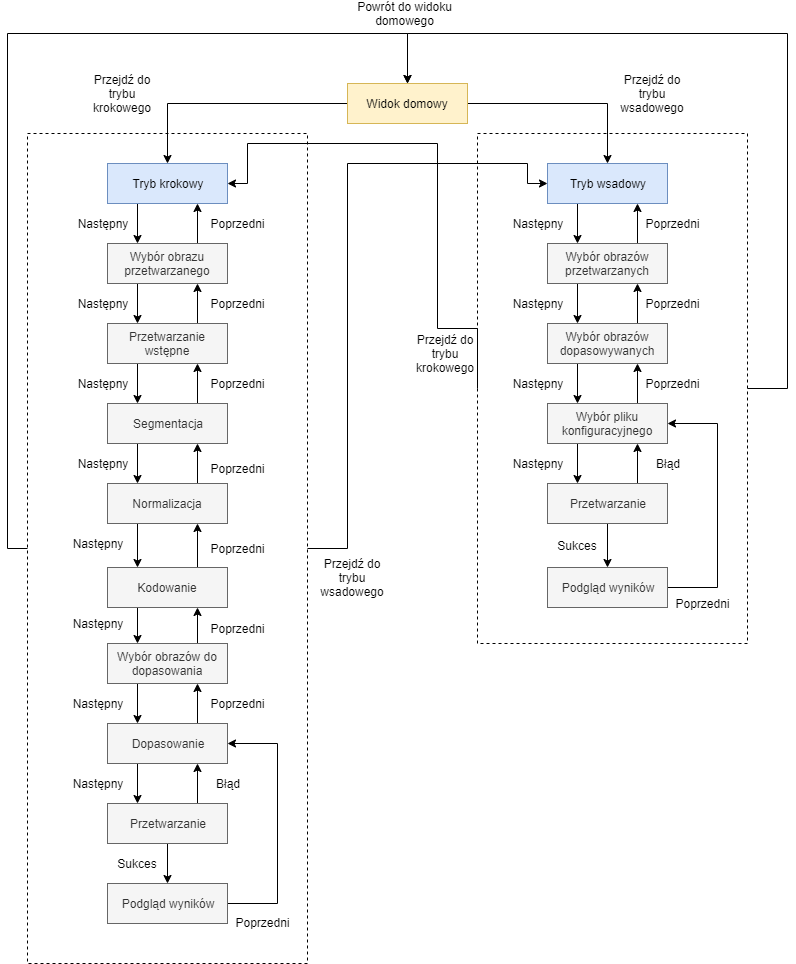
\includegraphics[width=\textwidth,height=\textheight, keepaspectratio]{images/widokiMgr.png}
    \caption{Diagram widoków i przejś\'c aplikacji.}
\end{figure}

\chapter{Zaimplementowane algorytmy}

Zgodnie z założeniami w niniejszej pracy zaimplementowane zostały rozwiązania dla następujących
etapów procesu rozpoznawania tęczówki:

\begin{itemize}
  \item przetwarzanie wstępne,
  \item normalizacja,
  \item kodowanie,
  \item dopasowanie.
\end{itemize}

\noindent
Algorytmy segmentacji tęczówki oraz usuwania zakłóceń zostały pominięte, ponieważ były przedmiotem
innej pracy dyplomowej. W dalszej części rozdziału opisane zostaną zaimplementowane algorytmy
dla wyżej wymienionych etapów.

\section{Przetwarzanie wstępne}

Odpowiednie przygotowanie obrazu przed rozpoczęciem procesu rozpozanawania jest bardzo ważne. Pozwala
ono na polepszenie jakości zdjęcia przez usunięcie zakłóceń czy poprawienie kontrastu, co znacznie
wpływa na jakoś\'c działania całego systemu.\newline

Różne metody segmentacji wymagają odmiennego wstępnego przygotowania obrazu. Często proces przygotowania
obrazu różni się nawet dla poszczególnych etapów procesu segmentacji, tzn. innych operacji może wymaga\'c
obraz w trakcie szukania parametrów źrenicy, a jeszcze innego w trakcie szukania parametrów tęczówki.
Z tego względu przetwarzanie wstępne może byc doś\'c skomplikowane i składac się z wielu różnorodnych
kroków.

Ponieważ algorytmy segmentacji często polegają na konkretnych operacjach przygotowawczych, których może
by\'c wiele, umożliwienie użytkownikowi ich parametryzacji bardzo skomplikowałoby interfejs aplikacji
i znacznie pogorszyło by jego czytelnoś\'c, jednocześnie dając użytkownikowi niewiele pola do manipulacji
tą częścią procesu.\newline

Ze względu na zależnoś\'c procesu przygotowania obrazu od wybranego algorytmu segmentacji, implementacja
przetwarzania wstępnego przeniesiona została do implementacji poszczególnych metod segmentacji,
a użytkownikowi udostępnione zostały wyłącznie uniwersalne algorytmy takie jak:

\begin{itemize}
  \item filtr Gaussa
  \item filtr medianowy
  \item normalizacja histogramu
  \item filter2D
\end{itemize}

Implementacje tych alogrytmów wykorzystują podstawowe funkcje z biblioteki OpenCV takie jak:
\verb|GaussianBlur|, \verb|medianBlur|, \verb|equalizeHist| oraz \verb|filter2D|.

\section{Normalizacja}

Porównywanie tęczówki może by\'c problematyczne, ze względu na potencjalne niezgodności w
wymiarach obrazu. Najczęstszą przyczyną tych niespójności jest zmiana rozmiaru tęczówki
będąca wynikiem rozszerzania lub kurczenia się  \'zrenicy oka w zależności od intensywności
oświetlenia w otoczeniu. Niespójności te mogą wynika\'c również z innych \'zródeł np. różna
odległoś\'c w trakcie pobierania zdjęcia, różnice w obrocie kamery, inna rotacja oka, czy
nawet nachylenie głowy w trakcie pobierania zdjęcia \cite{DaugmanHowIrisRecognitionWorks}.\newline

W celu umożliwienia porównania dwóch obrazów, z których każde mogło by\'c zrobione w odmiennych
warunkach, obraz poddaje się procesowi normalizacji, który ma za zadanie uspójni\'c rozmiary
tęczówki w systemie.

\noindent
Ważną informacją dla procesu normalizacji jest także to, że środek \'zrenicy i tęczówki nie
muszą znajdowa\'c się w tym samym punkcie, co musi by\'c wzięte pod uwagę przy opracowywaniu
rozwiązania.\newline

W aplikacji zdecydowano się na użycie normalizacji metodą Daugmana \cite{DaugmanHowIrisRecognitionWorks}, która polega na przekształceniu
obrazu tęczówki z postaci pierścienia do postaci prostokąta przez zmianę układu współrzędnych, w którym
prezentowane są wartości poszczególnych punktów tęczówki. Zmiana ta polega na przejściu z opisu
wartości pikseli w kartezjańskim układzie współrzędnych $(x,y)$, do opisu za pomocą pary
współrzędnych biegunowych $(r, \theta)$, gdzie r jest wartością z przedziału $[0,1]$, a $\theta$ jest kątem
z przedziału $[0, 2\pi]$.\newline

\begin{figure}[ht]
  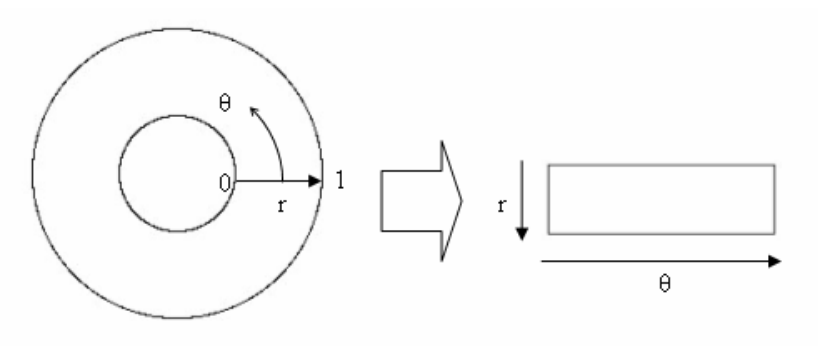
\includegraphics[width=0.8\textwidth]{images/normalization/schemaCenter.png}
  \centering
  \caption{Model normalizacji Daugmana \cite{masek}}
  \label{fig:daugmanDiagram}
\end{figure}

Wybrany rozmiar prostokąta decyduje o ilości informacji znajdujących się w znormalizowanym obrazie.
Wiersze w tak uzyskanym prostokącie można interpretowa\'c jako kolejne okręgi na obrazie tęczówki.
Jak wida\'c na powyższym rysunku \ref{fig:daugmanDiagram}, wybrana wysokoś\'c prostokąta decyduje
o ilości okręgów - rozdzielczoś\'c promieniowa , a szerokoś\'c prostokąta decyduje o rozdzielczości kątowej.\newline

Przejście ze współrzędnych kartezjańskich $(x,y)$ do współrzędnych biegunowych $(r,\theta)$ opisane zostało
przez Daugmana \cite{DaugmanHowIrisRecognitionWorks} równaniami \ref{eq:norm}:

\begin{equation}
  \begin{aligned}
    &I(x(r,\theta), y(r,\theta)) \rightarrow I(r,\theta),
    \\
    \\
    &x(r,\theta) = (1-r)x_{p}(\theta) + rx_{s}(\theta),
    \\
    &y(r,\theta) = (1-r)y_{p}(\theta) + ry_{s}(\theta),
  \end{aligned}
  \label{eq:norm}
\end{equation}

\noindent
gdzie:\\
\indent $x_{p}$, $y_{p}$ - współrzędne na okręgu granicznym \'zrenicy wzdłuż kierunku $\theta$,\\
\indent $x_{s}$, $y_{s}$ - współrzędne na okręgu granicznym tęczówki wzdłuż kierunku $\theta$.\newline

Tak jak wcześniej wspomniano, środki \'zrenicy i tęczówki nie zawsze znajdują się na jednej osi.
Z tego względu wyznaczając kolejne punkty znormalizowanego obrazu należy uwzględni\'c różną odległoś\'c
między granicą \'zrenicy a tęczówki w zależności od rozpatrywanego kąta $\theta$, co dobrze zobrazowane
zostało na rysunku \ref{fig:daugmanDiagramOffCenter}. Niezależnie od tych różnic, wzdłuż każdego kierunku
$\theta$ wybierana jest stała liczba punktów w taki sposób, aby otrzymany obraz był prostokątem
o stałych wymiarach.

\begin{figure}[ht]
  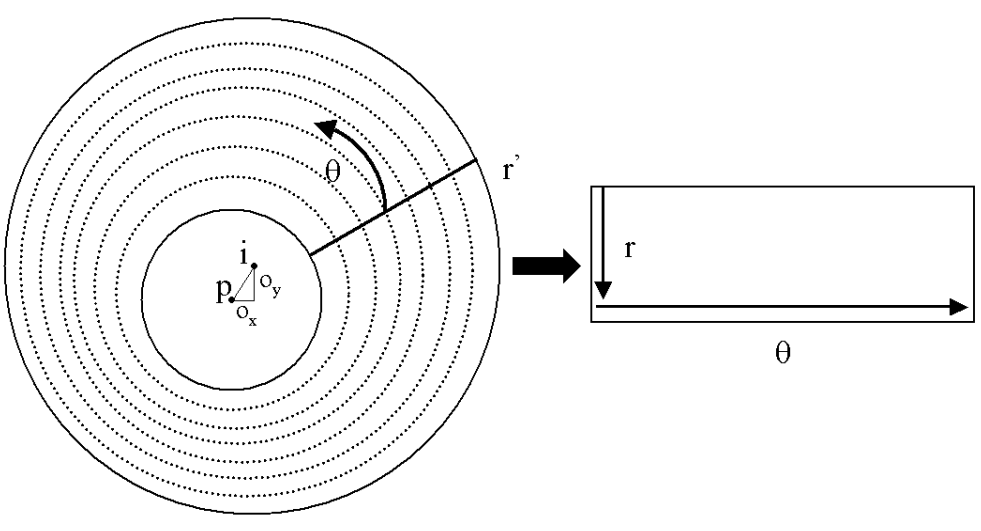
\includegraphics[width=0.8\textwidth]{images/normalization/schemaOffCenter.png}
  \centering
  \caption{Model normalizacji Daugmana z uwzględnieniem niewspółosiowości tęczówki i \'zrenicy \cite{aliasingIris}}
  \label{fig:daugmanDiagramOffCenter}
\end{figure}

Uwzględnienie tej niewspółosiowości polega na wyznaczeniu wartości odległości między granicami
\'zrenicy i tęczówki dla każdego rozpatrywanego kąta \cite{masek} zgodnie z równaniami \ref{eq:normRemap}.

\begin{equation}
  \begin{aligned}
    &r^{\prime} = \sqrt{\alpha}\beta \pm \sqrt{\alpha\beta^{2} - \alpha - r_{I}^{2}},
    \\
    \\
    &\alpha = o_{x}^{2} + o_{y}^{2},
    \\
    &\beta = \cos \left( \pi - \arctan \left( \frac{o_{y}}{o_{x}} \right) - \theta \right).
  \end{aligned}
  \label{eq:normRemap}
\end{equation}

\noindent
gdzie:\\
\indent $o_{x}, o_{y}$ - różnica położeń między środkiem \'zrenicy i tęczówki,\\
\indent $r^{\prime}$ - odległoś\'c między granicą \'zrenicy, a granicą tęczówki pod kątem $\theta$,\\
\indent $r_{I}$ - promień tęczówki\newline

Jeżeli w procesie segmentacji wygenerowana została dodatkowo maska zawierająca informacje o
zakłoceniach znajdujących się w obrębie tęczówki, takich jak powieki, czy rzęsy, wygenerowaną
maskę również należy podda\'c procesowi normalizacji, aby umożliwi\'c korzystanie z niej podczas
porównywania tęczówek. Przykład procesu normalizacji przedstawiony został na rysunku \ref{fig:normalizationExample}.

\begin{figure}[ht]
  \centering
  \begin{subfigure}[b]{0.35\textwidth}
    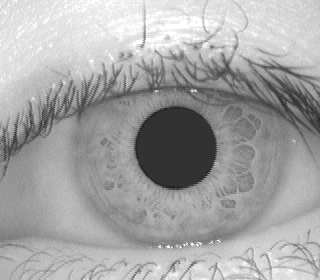
\includegraphics[width=\textwidth]{images/normalization/original.png}
    \caption{Obraz oryginalny}
  \end{subfigure}
  \begin{subfigure}[b]{0.35\textwidth}
    
\includegraphics[width=\textwidth]{images/normalization/mask.png}
    \caption{Maska zakłóceń}
  \end{subfigure}
  \begin{subfigure}[b]{0.35\textwidth}
    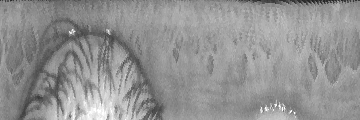
\includegraphics[width=\textwidth]{images/normalization/irisNormalized.png}
    \caption{Tęczówka po normalizacji}
  \end{subfigure}
  \begin{subfigure}[b]{0.35\textwidth}
    
\includegraphics[width=\textwidth]{images/normalization/maskNormalized.png}
    \caption{Maska zakłóceń po normalizacji}
  \end{subfigure}
  \caption{Przykład normalizacji metodą Daugmana}
  \label{fig:normalizationExample}
\end{figure}

Takie rozwiązanie zapewnia odpornoś\'c na rozszerzanie i kurczenie się \'zrenicy, niewspółosiowoś\'c
okręgów tęczówki i \'zrenicy a także różnicę położenia ich między różnymi obrazami. Metoda ta nie
kompensuje jednak różnic rotacji tęczówki. Kompensacja ta jest natomiast zapewniana w procesie
dopasowywania obrazów, który opisany został w pó\'zniejszej części tego rozdziału.

\section{Kodowanie}

Kodowanie tęczówki można rozumie\'c jako opis jej cech.
Dobry algorytm ekstrakcji cech sprawi, że wynik miary dopasowania dla obrazów tej samej tęczówki
będzie znajdował się w innym przedziale niż podczas porównywania obrazów dwóch
różnych tęczówek. Dzięki temu w końcowym etapie procesu rozpoznawania możliwe jest podjęcie decyzji
o rozpoznaniu bąd\'z nierozpoznaniu tęczówki.

Aby zapewni\'c dobrą jakoś\'c identyfikacji tęczówki, proces kodowania powinien wyciąga\'c
z obrazu tylko najważniejsze i najbardziej rozróżnialne jego cechy.
Oppenheim i Lim \cite{OppenheimLim} pokazali w swojej pracy, że najważniejsze
cechy obrazu niesie ze sobą widmo fazowe. Widmo amplitudowe zawiera
informacje o mniej indywidualnych cechach, a także jest zależne od czynników zewnętrznych takich
jak kontrast czy oświetlenie. Z tego względu podczas kodowania tęczówki wykorzystane
powinno by\'c właśnie widmo fazowe obrazu. W celu jego uzyskania należy przenieś\'c znormalizowany
obraz z dziedziny przestrzennej do dziedziny częstotliwości.\newline

Daugman \cite{DaugmanHowIrisRecognitionWorks} w swojej pracy zaproponował użycie w tym celu
filtrów Gabora, dzięki którym można uzyska\'c połączoną reprezentację obrazu w przestrzeni
oraz częstotliwości. Filtry te powstają w wyniku modulacji sinusoidy oraz cosinusoidy za pomocą
funkcji Gaussowskiej.
Częstotliwoś\'c środkowa filtru wyznaczana jest przez częstotliwoś\'c sinusoidy, natomiast
przepustowoś\'c filtru określana jest przez szerokoś\'c wykorzystanej funkcji Gaussowskiej.

Jedną z wad filtrów Gabora jest występowanie niezerowej składowej stałej dla przepustowości
większej niż jedna oktawa \cite{FieldGaborOctave}. Zerową składową stałą dla każdej przepustowości
można natomiast otrzyma\'c przez zastosowanie filtru, którego charakterystyka częstotliwościowa
amplitudowa ma rozkład Gaussowski nie w skali liniowej, a w skali logarytmicznej. Charakterystyka
częstotliwościowa amplitudowa takiego filtru jest opisana równaniem \ref{eq:logGabor}:

\begin{equation}
  \mathit{G(f)} = \exp\left(
  \frac{
    -\left( \log\left( f / f_{0}\right)\right)^{2}
  }{
    2\left(\log\left( \sigma / f_{0}\right)\right)^{2}
  }
  \right),
  \label{eq:logGabor}
\end{equation}

\noindent
gdzie:\\
\indent $f_{0}$ - częstotliwoś\'c środkowa filtra,\\
\indent $\sigma$ - przepustowoś\'c filtra.\newline

W celu zakodowania cech charakterystycznych znormalizowanego obrazu tęczówki, dla każdego wiersza
obrazu obliczany jest jego splot z falkami Log Gabora. Jeżeli moduł wyniku splotu w danym punkcie
jest bardzo blisko zera, wówczas informacja fazowa jest nieznacząca, a punkt ten oznaczany jest w
masce zakłóceń jako bit nieznaczący.

Wynik splotu obrazu z filtrem jest następnie poddawany kwantyzacji \cite{DaugmanHowIrisRecognitionWorks} do czterech wartości odpowiadających
czterem \'cwiartkom płaszczyzny zespolonej przez sprawdzenie znaku częsci rzeczywistej i urojonej
uzyskanego wyniku. Proces kwantyzacji przedstawiony jest na rysunku \ref{fig:encodingQuant}. W wyniku
kwantyzacji znormalizowany obraz tęczówki przekształcany jest do wzoru tęczówki w postaci ciągu bitów.
Przykładowy proces kodowania przedstawiony został na rysunku \ref{fig:gaborEncoding}

\begin{figure}[ht]
  \centering
  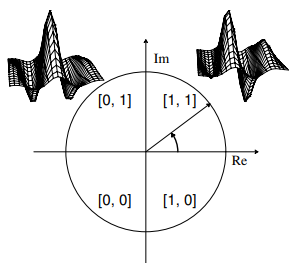
\includegraphics{images/encoding/quantization.png}
  \caption{Ilustracja procesu kwantyzacji}
  \label{fig:encodingQuant}
\end{figure}

W celu uzyskania większej ilości informacji o tęczówce możliwe jest zastosowanie kilku filtrów
Gabora o różnych parametrach. Wówczas obraz poddawany jest splotowi z każdym z takich filtrów, w
związku z czym powielana jest liczba bitów kodujących każdy punkt tęczówki.

Z każdym punktem na obrazie tęczówki związana jest pojedyńcza wartoś\'c w masce zakłóceń. W wyniku
procesu kodowania każdy element obrazu jest reprezentowany przez przynajmniej dwie wartości. W związku
z tym należy zaktualizowa\'c maskę zakłóceń, aby miała ona ten sam rozmiar co otrzymany wzór tęczówki.
W tym celu każdy bit w masce zakłóceń jest powielany tyle razy, ile wartości reprezentuje pojedyńczy
punkt we wzorze tęczówki. Przykładowo, jeżeli w procesie kodowania wykorzystany został jeden filtr,
transformacja przykładowej maski wyglądałaby następująco:

\begin{figure}[ht]
  \centering
  $0|1|1|0|0|1 \rightarrow 00|11|11|00|00|11$
\end{figure}

\begin{figure}[!ht]
  \centering
  \makebox[\textwidth]{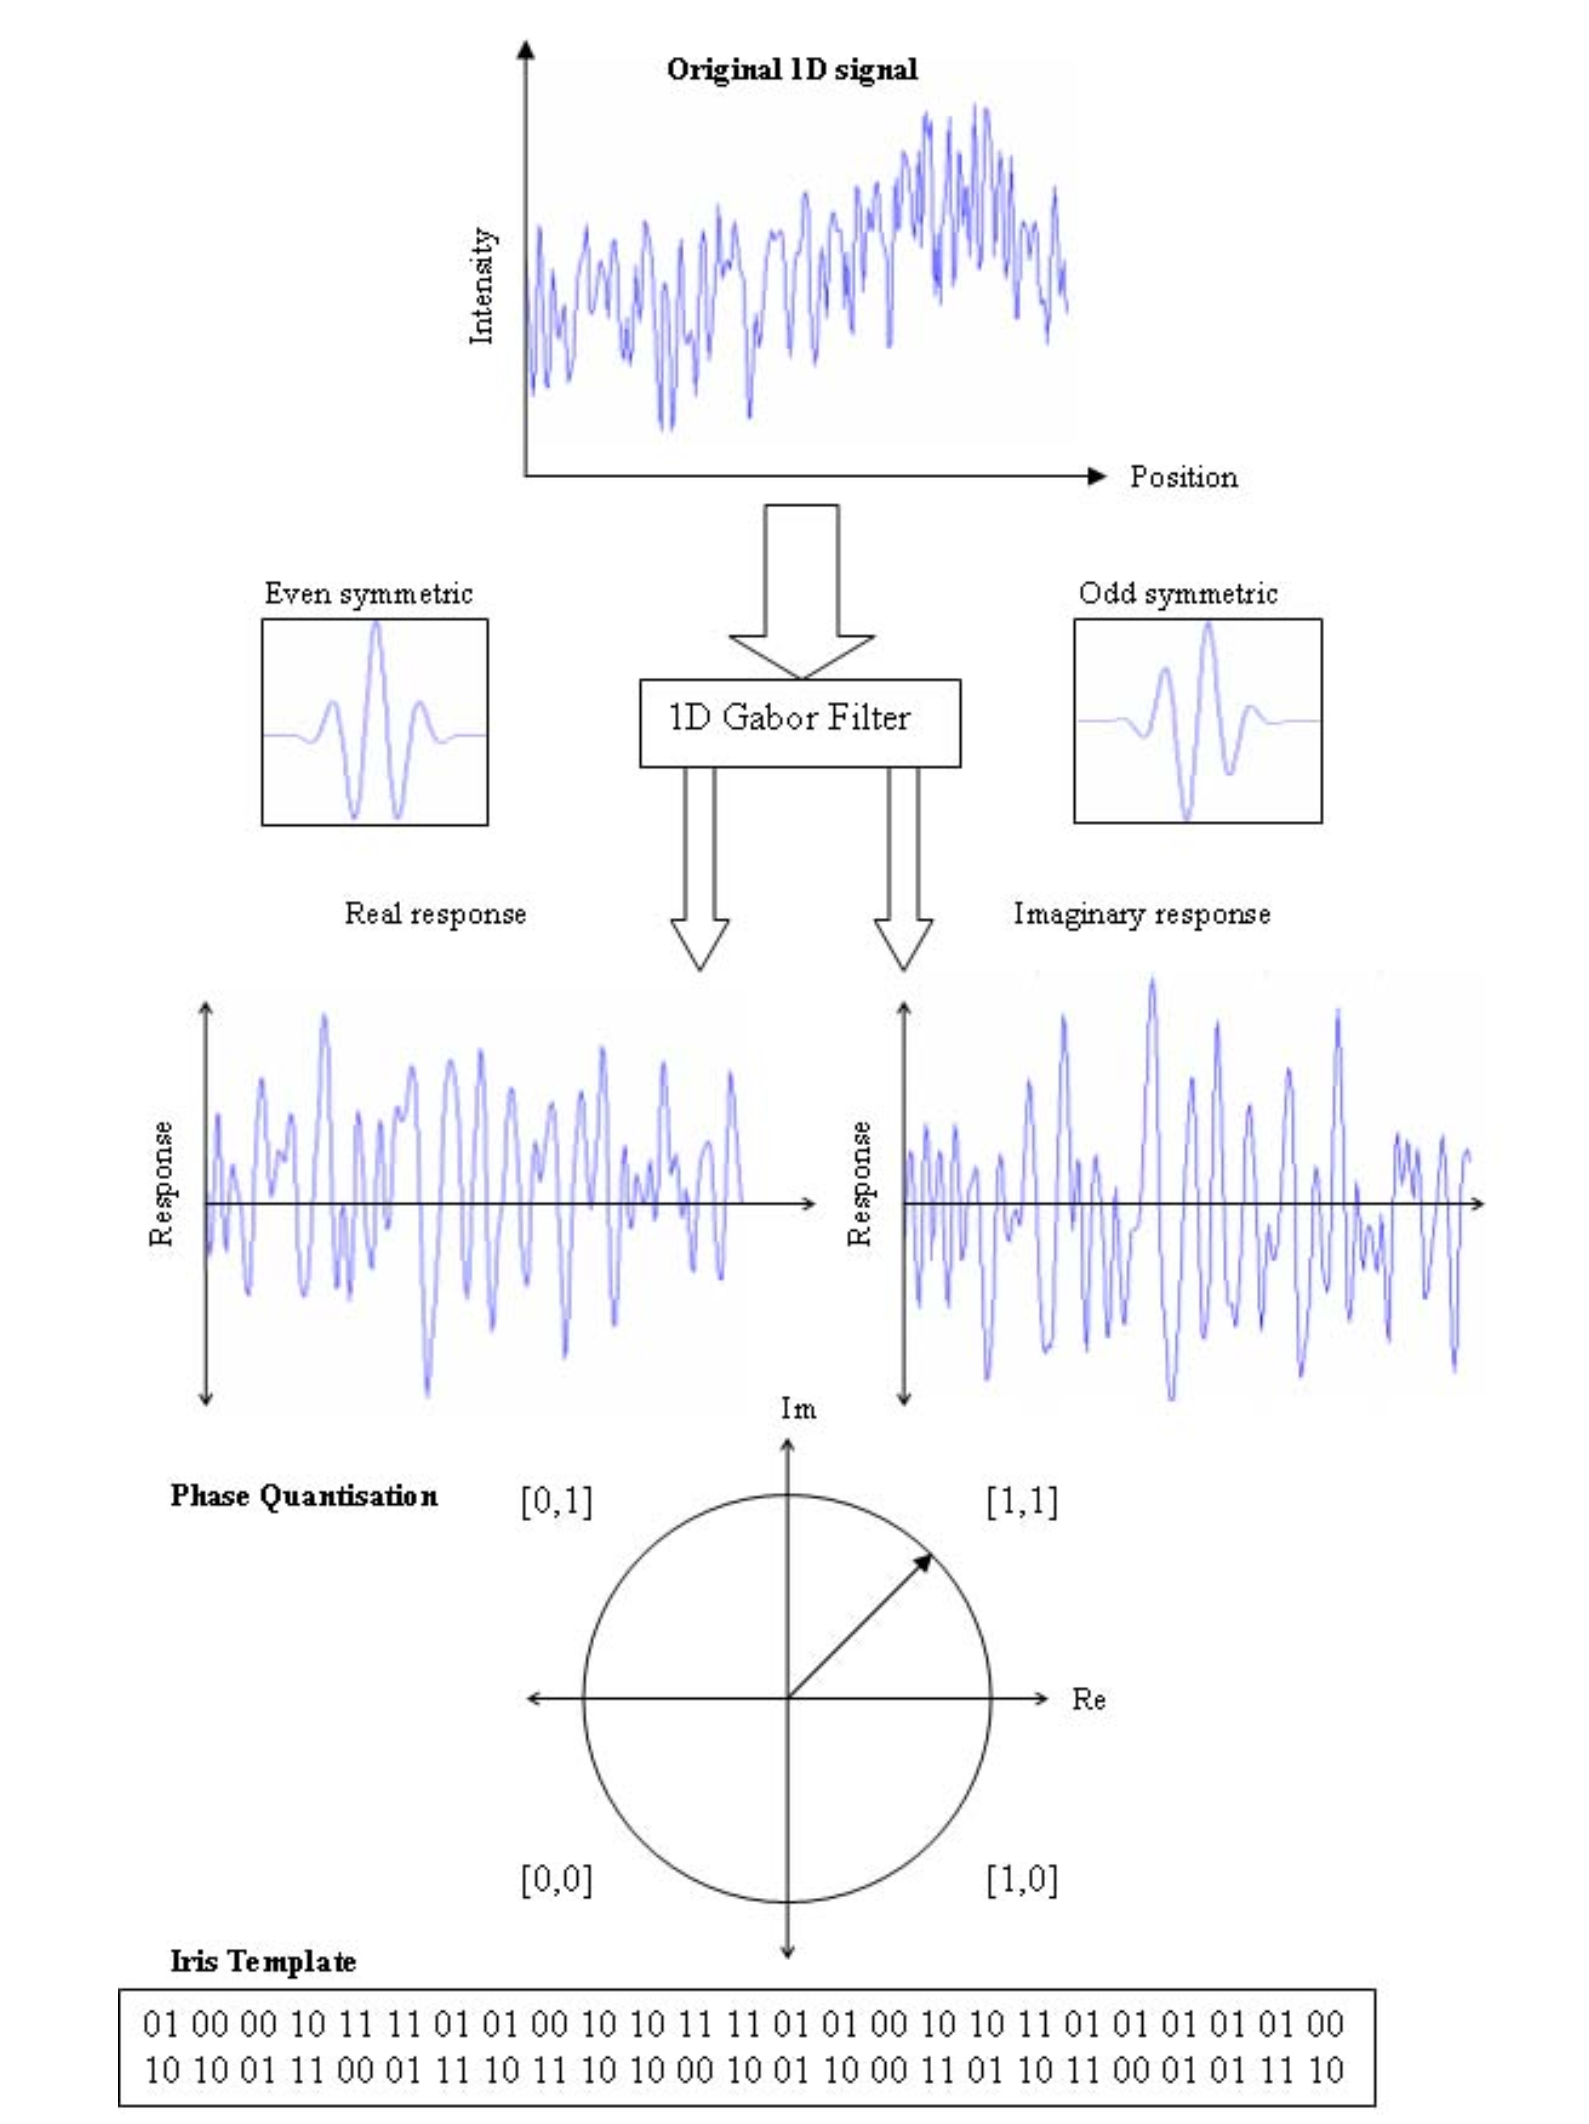
\includegraphics[width=\textwidth,height=\textheight,keepaspectratio]{images/encoding/gabor.png}}
  \caption{Ilustracja procesu kodowania}
  \label{fig:gaborEncoding}
\end{figure}

Na rysunku \ref{fig:gaborExample} przestawiony został przykładowy wynik procesu kodowania zaimplementowanego
w tej pracy.

\begin{figure}
  \centering
  \begin{subfigure}[b]{0.5\textwidth}
    
\includegraphics[width=\textwidth]{images/encoding/norm.png}
    \caption{Znormalizowany obraz tęczówki}
  \end{subfigure}
  \begin{subfigure}[b]{0.5\textwidth}
    
\includegraphics[width=\textwidth]{images/encoding/normMask.png}
    \caption{Znormalizowana maska zakłóceń}
  \end{subfigure}
  \begin{subfigure}[b]{1\textwidth}
    
\includegraphics[width=\textwidth]{images/encoding/encoded.png}
    \caption{Wzór tęczówki obrazu znormalizowanego}
  \end{subfigure}
  \begin{subfigure}[b]{\textwidth}
    
\includegraphics[width=\textwidth]{images/encoding/encodedMask.png}
    \caption{Dostosowana maska zakłóceń do nowego rozmiaru}
  \end{subfigure}
  \caption{Wyniki przykładowego kodowania za pomocą filtrów Gabora.}
  \label{fig:gaborExample}
\end{figure}

\section{Dopasowanie}

W procesie kodowania obraz tęczówki przekształcony zostaje do wzoru tęczówki w postaci ciągu bitowego,
dzięki czemu porównanie dwóch obrazów tęczówek sprowadza się do porównania dwóch ciągów bitowych.
Stopień różnicy między dwoma wzorami tęczówki, można określi\'c obliczając odległoś\'c Hamminga. Mówi
ona o liczbie miejsc, w których dwa słowa bitowe przyjmują różne wartości.
Ustalając pewien próg wartości odległości Hamminga można podją\'c decyzję, czy dwa dane ciągi
reprezentują tę samą tęczówkę.

Wyznaczenie progu dla odległości Hamminga zdefiniowanej w ten sposób zależałoby od długości
porównywanych ciągów bitowych. Aby uniezależni\'c wartoś\'c progu od tej długości, miarę można
zdefiniowa\'c jako sumę niezgodnych bitów podzieloną przez całkowitą liczbę bitów \ref{eq:basicHD}:

\begin{equation}
  \mathit{HD} = \frac{1}{N}\sum\limits_{j=1}^{N}X_{j} \oplus Y_{j},
  \label{eq:basicHD}
\end{equation}

\noindent
gdzie:\\
\indent $X_{j}, Y_{j}$ reprezentują wartości bitów na miejscu $j$ w ciągach odpowiednio $X$ oraz $Y$,\\
\indent $N$ - długoś\'c ciągów $X$ i $Y$,\\
\indent $\oplus$ - operator alternatywy rozłącznej.\newline

W trakcie procesu kodowania oprócz wzoru tęczówki tworzony jest także wzór dla maski zakłóceń.
Zawiera on informacje o tym, które bity we wzorze tęczówki reprezentują tęczówkę i powinny by\'c
uwzględnione, a które bity reprezentują zakłócenia takie jak powieki, czy rzęsy i nie powinny by\'c
porównywane w procesie dopasowywania.\\
Jako że porównywane są dwa obrazy, generowane są również dwie maski zakłóceń i należy uwzględni\'c
każdą z nich. Ponieważ elementy znaczące w masce zakłóceń oznaczone zostały kolorem białym, co odpowiada
wartości $1$ w postaci bitowej. Ostateczną maskę dla procesu dopasowania można zdefiniowa\'c jako
iloczyn logiczny tych dwóch masek - w ten sposób stworzony zostanie jeden ciąg bitowy reprezentujący
bity znaczące za pomocą wartości $1$ oraz bity nieznaczące za pomocą wartości $0$.
Równanie \ref{eq:maskedHD} przedstawia definicję odległości Hamminga z uwzględnieniem obu masek zakłóceń:

\begin{equation}
  \mathit{HD} = \frac{1}{\sum\limits_{j=1}^{N} \left( \mathit{Xm}_{j} \cap \mathit{Ym}_{j} \right) }
       \sum\limits_{k=1}^{N} \left(X_{k} \oplus Y_{k} \right) \cap \left( \mathit{Xm}_{k} \cap \mathit{Ym}_{k} \right),
  \label{eq:maskedHD}
\end{equation}

\noindent
gdzie:\\
\indent $X, Y$ - wzory tęczówki,\\
\indent $\mathit{Xm}, \mathit{Ym}$ - wzory masek zakłóceń dla wzorów tęczówek $X, Y$,\\
\indent $N$ - długoś\'c wzorów tęczówek i masek zakłóceń,\\
\indent $\oplus$ - operator alternatywy rozłącznej,\\
\indent $\cap$ - operator iloczynu logicznego.\newline

Tak jak wcześniej wspomniano, poprzednie procesy w żaden sposób nie uwzględniały możliwości różnic
w rotacji tęczówki na pobranych obrazach. W celu kompensacji tych niespójności podczas procesu
dopasowania jeden z wzorów tęczówki poddawany jest przesunięciom bitowym, które odpowiadają rotacji
tęczówki o kąt zależny od rozdzielczości kątowej wybranej podczas procesu normalizacji. Maska zakłóceń
odpowiadająca temu wzorowi również poddawana jest tym przesunięciom.
Jedno przesunięcie w procesie dopasowania odpowiada dwóm przesunięciom bitowym - jednemu w lewo i
drugiemu w prawo, z których oba wykonywane są względem oryginalnego wzoru tęczówki. Proces ten
zobrazowany został na rysunku \ref{fig:matchingShifting}

\begin{figure}
  \centering
  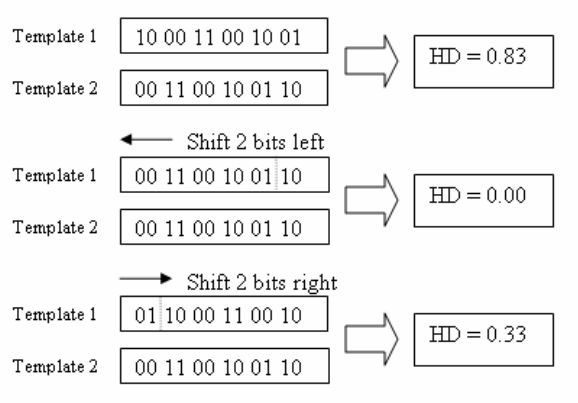
\includegraphics[width=0.6\textwidth]{images/matching/shifting.png}
  \caption{Schemat przedstawiający pojedyńcze przesunięcie wzoru tęczówki. Przykład ten przedstawia
  wzór do wygenerowania którego wykorzystany został jeden filtr Gabora \cite{masek}.}
  \label{fig:matchingShifting}
\end{figure}

W zależności od tego ile bitów koduje pojedyńczy punkt siatkówki, tyle bitów zmienia swoje miejsca
w trakcie pojedyńczego przesunięcia. Liczba przesuniętych bitów zależy od ilości filtrów Gabora
użytych w procesie kodowania, ponieważ każdy z takich filtrów wygeneruje dwa bity reprezentujące
pojedyńczy punkt siatkówki.

Odległos\'c Hamminga obliczana jest dla każdego z tych przesunię\'c. Decyzja o tym, czy dwa wzory
reprezentują tę samą tęczówkę podejmowana jest na podstawie najmniejszej uzyskanej wartości,
która reprezentuje najlepsze dopasowanie dwóch wzorów. Liczba przesunię\'c potrzebna do kompensacji
niespójności rotacji zależy od tego z jaką dokładnością kątową pobierane są zdjęcia tęczówki.

\chapter{Testy wydajnościowe}

\section{Wstęp}
 
W~poniższym rozdziale przedstawione zostaną wyniki testów wydajnościowych implementacji algorytmów
opisanych w~poprzedniej części pracy (poza algorytmem \emph{two-stage}, który został rozwinięty
i~poprawiony przez \emph{improved two-stage}). Implementacja w~języku \texttt{Java} została oparta
o~oryginalny kod, udostępniony przez autorów. Podstawą implementacji metody \emph{improved
two-stage} był kod algorytmu \emph{divsufsort} napisany przez Yutę Moriego [\ref{libdivsufsort}].

Algorytmy tworzenia tablic sufiksów zaimplementowane zostały w~ten sposób, żeby na wejściu
przyjmowały sekwencje liczb całkowitych typu \texttt{int} zajmujących w~języku \texttt{Java} 4
bajty. Spowodowało to zwiększenie złożoności pamięciowej algorytmów (wartości podane w~tabeli
\ref{tab:alg} zakładały wejście w~postaci sekwencji jednobajtowych elementów). Powodem zwiększenia
rozmiaru pojedynczego elementu wejściowego było umożliwienie tworzenia tablic sufiksów dla sekwencji
symboli z~alfabetów o~dużym rozmiarze. Nie jest to jednak możliwe w~praktyce w~przypadku wszystkich
algorytmów; rzeczywista złożoność pamięciowa implementacji wybranych metod oraz ich zależność od
rozmiaru alfabetu wejściowego opisane zostały w~tabeli \ref{tab:alg-impl}. Testowane implementacje
algorytmów \emph{bpr}, \emph{deep-shallow} i~\emph{qsufsort} dla zaoszczędzenia pamięci nadpisywały
ciąg wejściowy. Na potrzeby testów wydajnościowych zaimplementowano również naiwny algorytm
tworzenia tablic sufiksów opierający się o~zwykły algorytm sortujący \emph{quicksort}. W~dalszej
części rozdziału metoda naiwna nazywana będzie \emph{naive sort} lub NS.

Wykonane testy algorytmów można podzielić na dwie główne kategorie: testy na wejściu generowanym
losowo, oraz testy na wejściu wczytywanym z~plików. Testy drugiego typu wykonywane były na kilku
różnych maszynach wirtualnych:

\begin{itemize}
    \item maszyna Java HotSpot 64-Bit Server VM 11.0-b16 firmy Sun Microsystems, oznaczana w~dalszej części pracy jako \texttt{sun},
    \item maszyna IBM J9 VM 2.4 firmy IBM, oznaczana w~dalszej części pracy jako \texttt{ibm},
    \item BEA JRockit(R) R27.5.0-110\_o-99226-1.6.0\_03 firmy BEA (aktualnie przejęta przez Oracle), oznaczana w~dalszej części pracy jako \texttt{jrockit},
    \item Apache Harmony DRLVM 11.2.0 tworzona przez Apache Software Foundation, oznaczana w~dalszej części pracy jako \texttt{harmony}.
\end{itemize} 

\begin{table}[ht]
    \begin{center}        
        \begin{tabular}{l r r}
         \toprule
            Nazwa & Złożoność pamięciowa \\
         \midrule
            \emph{skew} & $16n$  \\
            \emph{bpr} & $4|\Sigma|^3+12n$ \\ 
            \emph{deep-shallow} & $4|\Sigma|^2+(x+8)n$  \\
            \emph{divsufsort} & $4|\Sigma|^2+8n$ \\
            \emph{qsufsort} & $8n$ \\
            \emph{naive sort} & $8n$ \\
        \bottomrule
        \end{tabular}
    \end{center}                         
    \caption{Zaimplementowane algorytmy tworzenia tablic sufiksów. Parametr $n$ oznacza długość wejścia, 
    parametr $|\Sigma|$ oznacza wielkość alfabetu sekwencji wejściowej. Algorytm \emph{deep-shallow} wymaga
    alfabetu o~rozmiarze nie większym niż 256, zużycie pamięci przez ten 
    algorytm zależy od wielkości budowanego drzewa \emph{blind trie}, które maksymalnie może zawierać $n$ elementów. Rozmiar jednego elementu drzewa wynosi $x=48$ bajtów na 64-bitowej maszynie wirtualnej firmy Sun.
    Algorytmy \emph{bpr} i~\emph{divsufsort} nie mają sztywnych ograniczeń na rozmiar 
    alfabetu, ale ze względu na wydajność nie powinny być używane na dużych alfabetach.}%
    \label{tab:alg-impl}
\end{table}
	
\noindent
Testy przeprowadzone zostały na kilku komputerach testowych o~następujących parametrach:
\begin{itemize}
    \item dwurdzeniowy procesor Athlon 5200 o~prędkości 2.6 GHz, 64-bitowy system operacyjny OpenSuSE, jądro w~wersji 2.6.22.19-0.2-default,
    \item czterordzeniowy procesor Intel Xeon x3230 o~prędkości 2.66 GHz, 64-bitowy system operacyjny OpenSuSE, wersja jądra 2.6.22.19-0.2-default,
    \item jednordzeniowy Intel Pentium 4 o~prędkości 3 GHz, 32-bitowy system operacyjny Windows XP.
\end{itemize}
	
\noindent
Wszystkie obliczenia przeprowadzone zostały z~parametrami maszyn wirtualnych
odpowiadającym opcjom ,,\texttt{-Xmx2g -server}'' -- zwiększają one maksymalny rozmiar 
sterty do 2Gb, a~maszyna wirtualna pracuje w~trybie ,,serwerowym'' (agresywna optymalizacja JIT).
	
Czas działania algorytmów mierzony był przez klasę uruchamiającą testy, poprzez liczenie różnicy
wartości zwracanych przez metodę \texttt{System.currentTimeMillis()} przed i~po obliczeniach
(tzw.~\emph{wall time}). Do mierzenia zużycia pamięci wykorzystano specjalnie w~tym celu napisany
aspekt [\ref{aspectj}]. Mierzone było zużycie pamięci wewnątrz wirtualnej maszyny na początku
działania algorytmu, pod jego koniec oraz po zakończeniu wybranych metod wewnątrz klas. Mierzenie
zużycia pamięci w~języku \texttt{Java} jest trudne, bowiem maszyna wirtualna nie pozwala na dokładne
oszacowanie wszystkich dokonanych alokacji pamięci. Do celów testowych posłużono się programowaniem
aspektowym i~,,wpleciono'' (\english{code weaving}) dynamiczne instrukcje mierzące różnicę
w~aktualnej ilości zaalokowanej pamięci względem startu algorytmu. Nie jest to oszacowanie idealne,
ale pozwala na zgrubne stwierdzenie ile pamięci zużywa dany algorytm.

Test na jednej instancji wejścia (pliku lub wygenerowanej sekwencji o~ustalonych parametrach)
powtarzany był 10 razy, a~jego wynikiem jest średnia z~zebranych pomiarów. Testy których wyniki
zbierano poprzedzano kilkoma uruchomieniami algorytmu. Celem tego zabiegu było wyeliminowanie błędów
pomiarowych wynikających z~wolniejszego działania kodu, który nie został skompilowany do kodu
natywnego przez maszynę wirtualną. Testy na wejściu generowanym losowo były poprzedzone 10 rundami
,,rozgrzewki", natomiast przed testem na wejściu wczytywanym z~pliku algorytm uruchamiany był 5
razy.
	
W~dalszej części rozdziału prezentowane są wyniki pochodzące z~pomiarów na komputerze z~procesorem
Xeon x3230. Wyniki z~pozostałych maszyn są niemal identyczne pod względem porównywania i~rankingu
algorytmów, dlatego też w wielu miejscach je pominięto (wszystkie wyniki są na dołączonej do pracy
płycie CD). Samo porównanie efektywności wykonania programów w różnych maszynach wirtualnych
znajduje się w rozdziale \ref{sect:vms}.


\section{Testy wydajnościowe na losowo generowanym wejściu}

Celem testów na losowo generowanym wejściu jest zbadanie rzeczywistej zależności algorytmów od
długości wejścia, wielkości alfabetu oraz średniego \emph{lcp} ciągu wejściowego. Testy
przeprowadzono tylko na jednej maszynie wirtualnej (\texttt{sun}). Ziarno generatora liczb losowych
otrzymywało identyczną wartość przed testem każdego algorytmu by zapewnić powtarzalność wyników.
	
	
\subsection{Wejście o~zmiennej długości i~stałej wielkości alfabetu}

Testy algorytmów na losowym wejściu o~zmiennej długości i~stałej wielkości alfabetu powtórzono trzy
razy. Każdy test wykonany był dla wejścia generowanego z~alfabetu wielkości 4,100 i~255 elementów.
Rysunek \ref{rys:random-input-lcp} przedstawia średnią wartość \emph{lcp} generowanych ciągów
wejściowych. Z~rysunku wynika, że wartość średniego \emph{lcp} jest mniej więcej odwrotnie
proporcjonalna do wielkości alfabetu.
		
Rysunki \ref{rys:random-input-time-4} i~\ref{rys:random-input-memory-4} przedstawiają czas działania
algorytmów oraz zużycie pamięci dla alfabetu wielkości 4. Algorytmy \emph{qsufsort} i~\emph{naive
sort} uzyskały najlepszy wynik złożoności pamięciowej. Zgodnie z~przewidywaniami, algorytmy
\emph{skew} i~\emph{deep shallow} wypadł najgorzej w~tej kwestii. Najszybszym algorytmem okazał się
być algorytm \emph{bpr}. Wyraźnie wolniejsze od pozostałych algorytmów są algorytmy \emph{skew}
i~\emph{naive sort}.


\begin{figure}[t]
       \begin{center}
            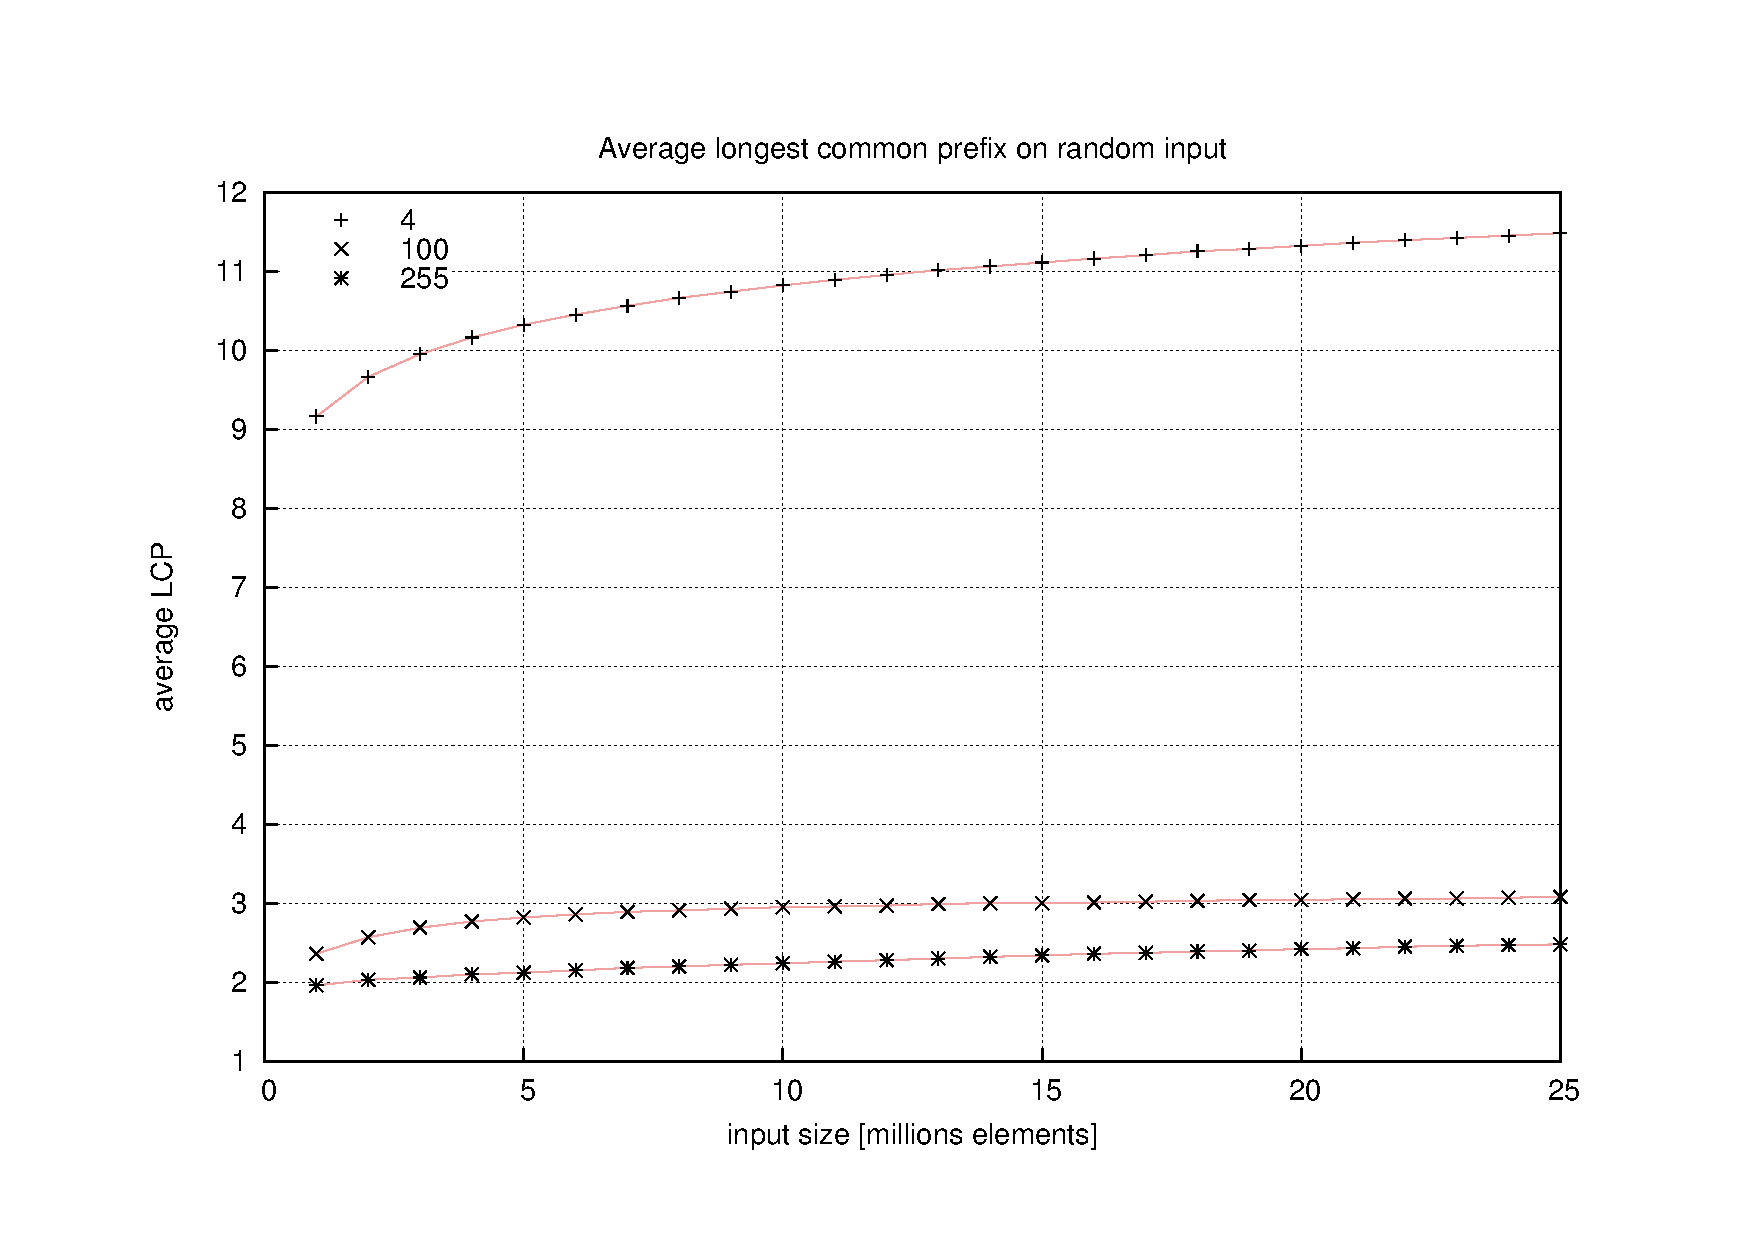
\includegraphics[width=\linewidth]{figures/results/random-input-lcp}
        \end{center}
    \caption{Średnie \emph{lcp} w~zależności od długości wejścia dla alfabetów o wielkości 4, 100 i~255 symboli.}%
    \label{rys:random-input-lcp}
\end{figure}

\begin{figure}[tp]
    \begin{center}
          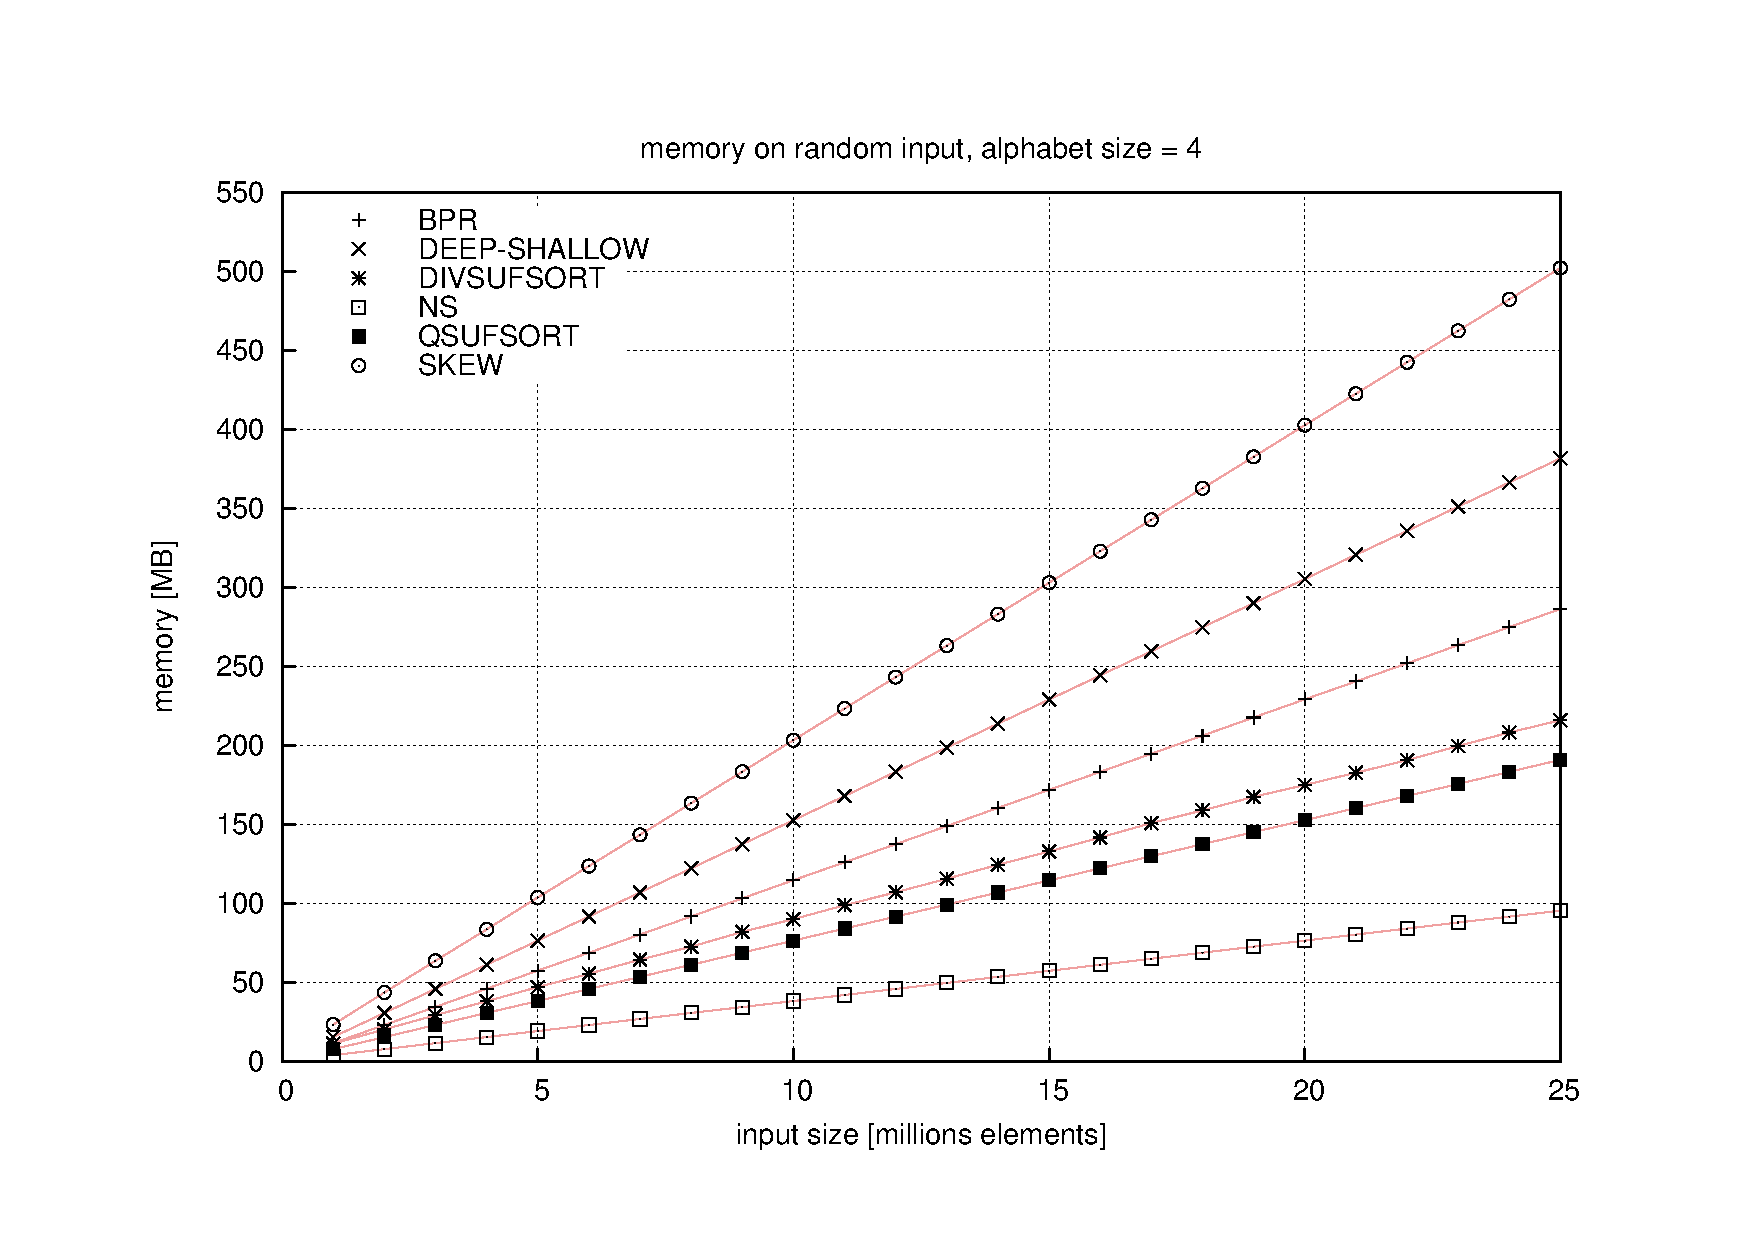
\includegraphics[width=\linewidth]{figures/results/random-input-memory-4}
    \end{center}
    \caption{Zużycie pamięci w~zależności od długości wejścia generowanego z~alfabetu wielkości 4.}%
    \label{rys:random-input-memory-4}
\end{figure}

%TODO wyniki zuzycia pamieci przez naive sort wskazuja na zaniżone wyniki pomiarów -- powinny być podobne wartości jak dla algorytmu qsufsort.
\begin{figure}[tp]
       \begin{center}
            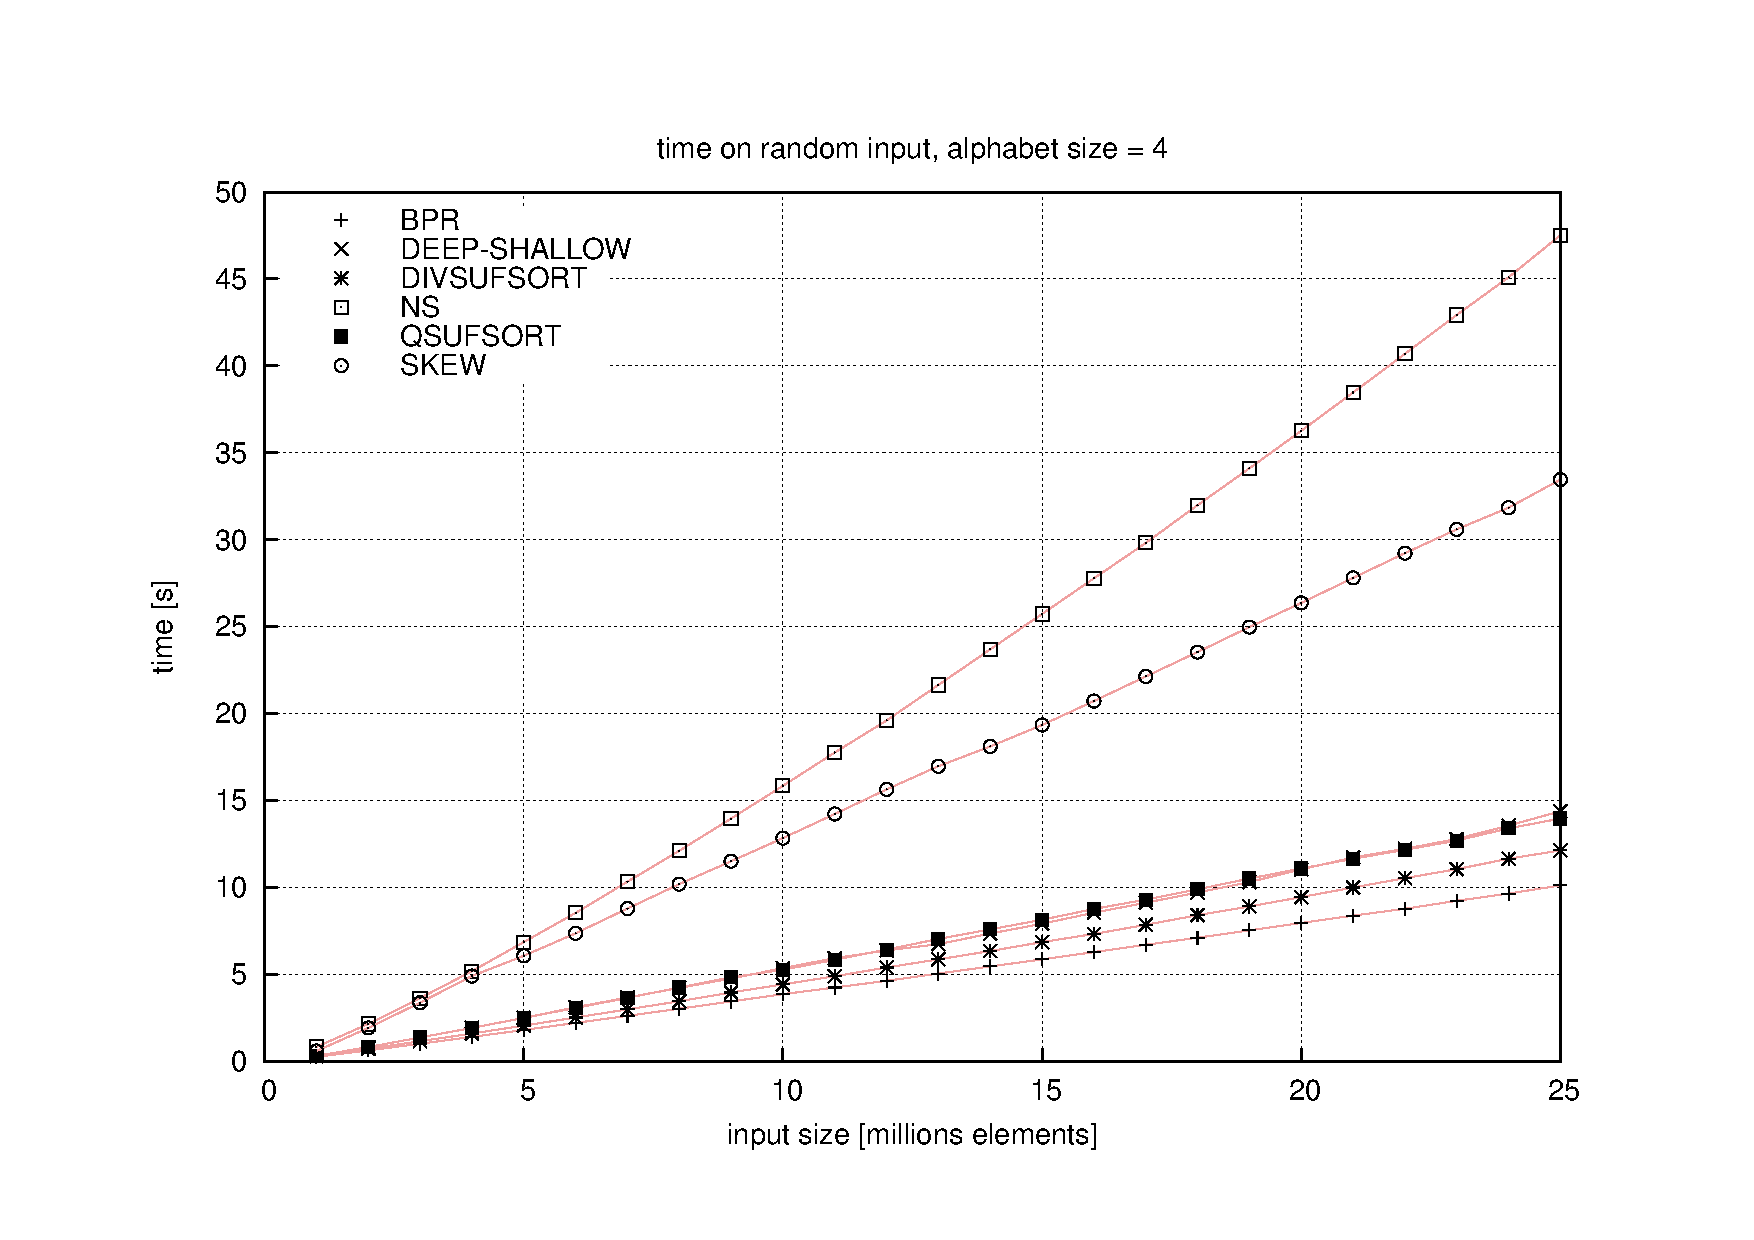
\includegraphics[width=\linewidth]{figures/results/random-input-time-4.pdf}
        \end{center}        
    \caption{Czas działania algorytmów w~zależności od długości wejścia generowanego z~alfabetu wielkości 4.}%
    \label{rys:random-input-time-4}
\end{figure}

\begin{figure}[tp]
   \begin{center}
      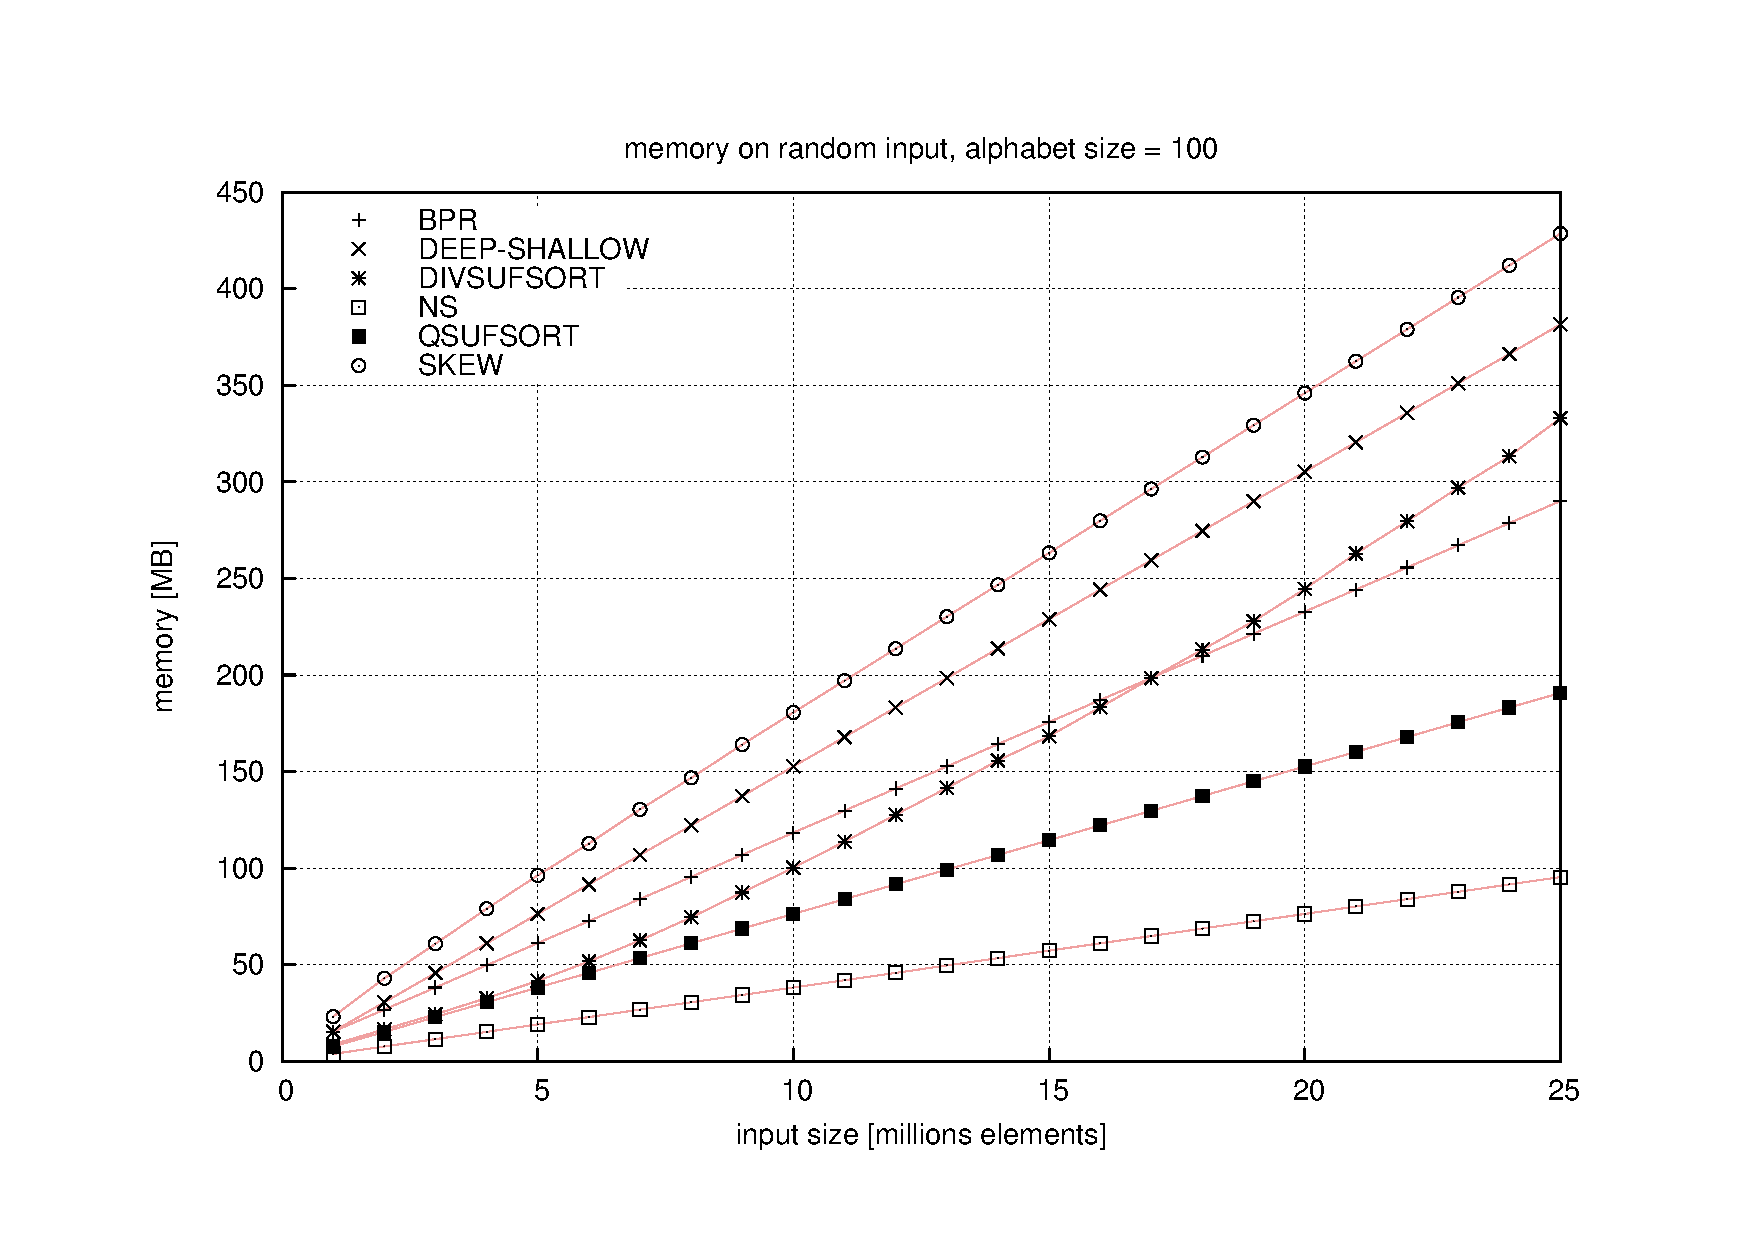
\includegraphics[width=\linewidth]{figures/results/random-input-memory-100.pdf}
    \end{center}        
    \caption{Zużycie pamięci w~zależności od długości wejścia generowanego z~alfabetu wielkości 100.}%
    \label{rys:random-input-memory-100}
\end{figure}

% nie wiem jak wyjaśnić zwiekszone zuzycie pamieci przez algorytm divsufsort
Wyniki testów wejścia generowanego z~alfabetu wielkości 100 przedstawione są na rysunku
\ref{rys:random-input-time-100} i~\ref{rys:random-input-memory-100}.
Rezultaty testu czasu działania algorytmu są niemal identyczne jak poprzedniego. Jedyną różnicą jest
to, że algorytm \emph{bpr} nie uzyskał najlepszego wyniku lecz znalazł się wśród kilku algorytmów
uzyskujących bardo dobry wynik, zajął również więcej pamięci.

\begin{figure}[tp]
   \begin{center}
        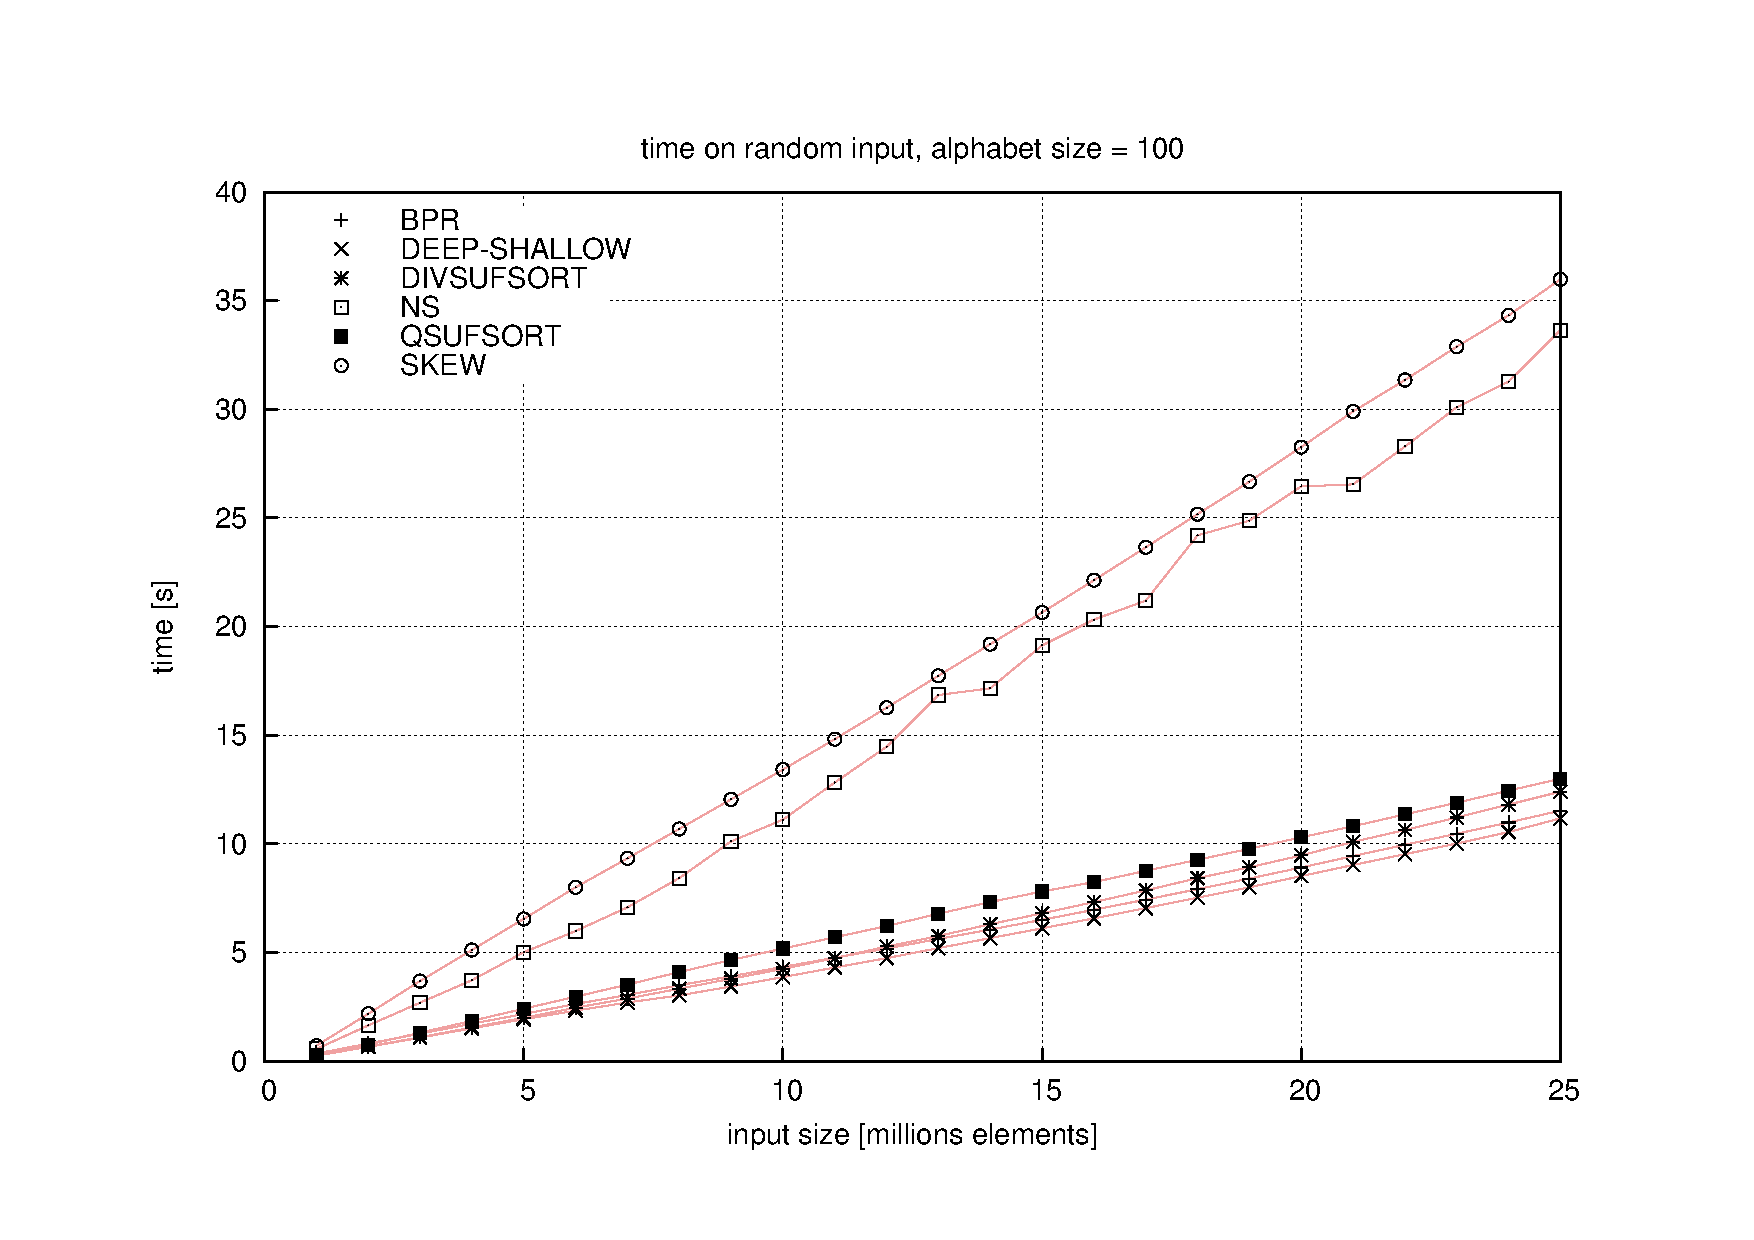
\includegraphics[width=\linewidth]{figures/results/random-input-time-100.pdf}
    \end{center}        
    \caption{Czas działania algorytmów w~zależności od długości wejścia generowanego z~alfabetu wielkości 100.}%
    \label{rys:random-input-time-100}
\end{figure} 

Rysunki \ref{rys:random-input-time-255} i~\ref{rys:random-input-memory-255} prezentują wyniki testów
wejścia generowanego z~alfabetu wielkości 255. Wynik tego testu są również podobne do poprzedników.
Algorytm \emph{bpr} uzyskał jeszcze gorszy wynik niż w~poprzednich testach, zajął więcej pamięci
i~działał wolniej od większości algorytmów.

\begin{figure}[tp]
       \begin{center}
          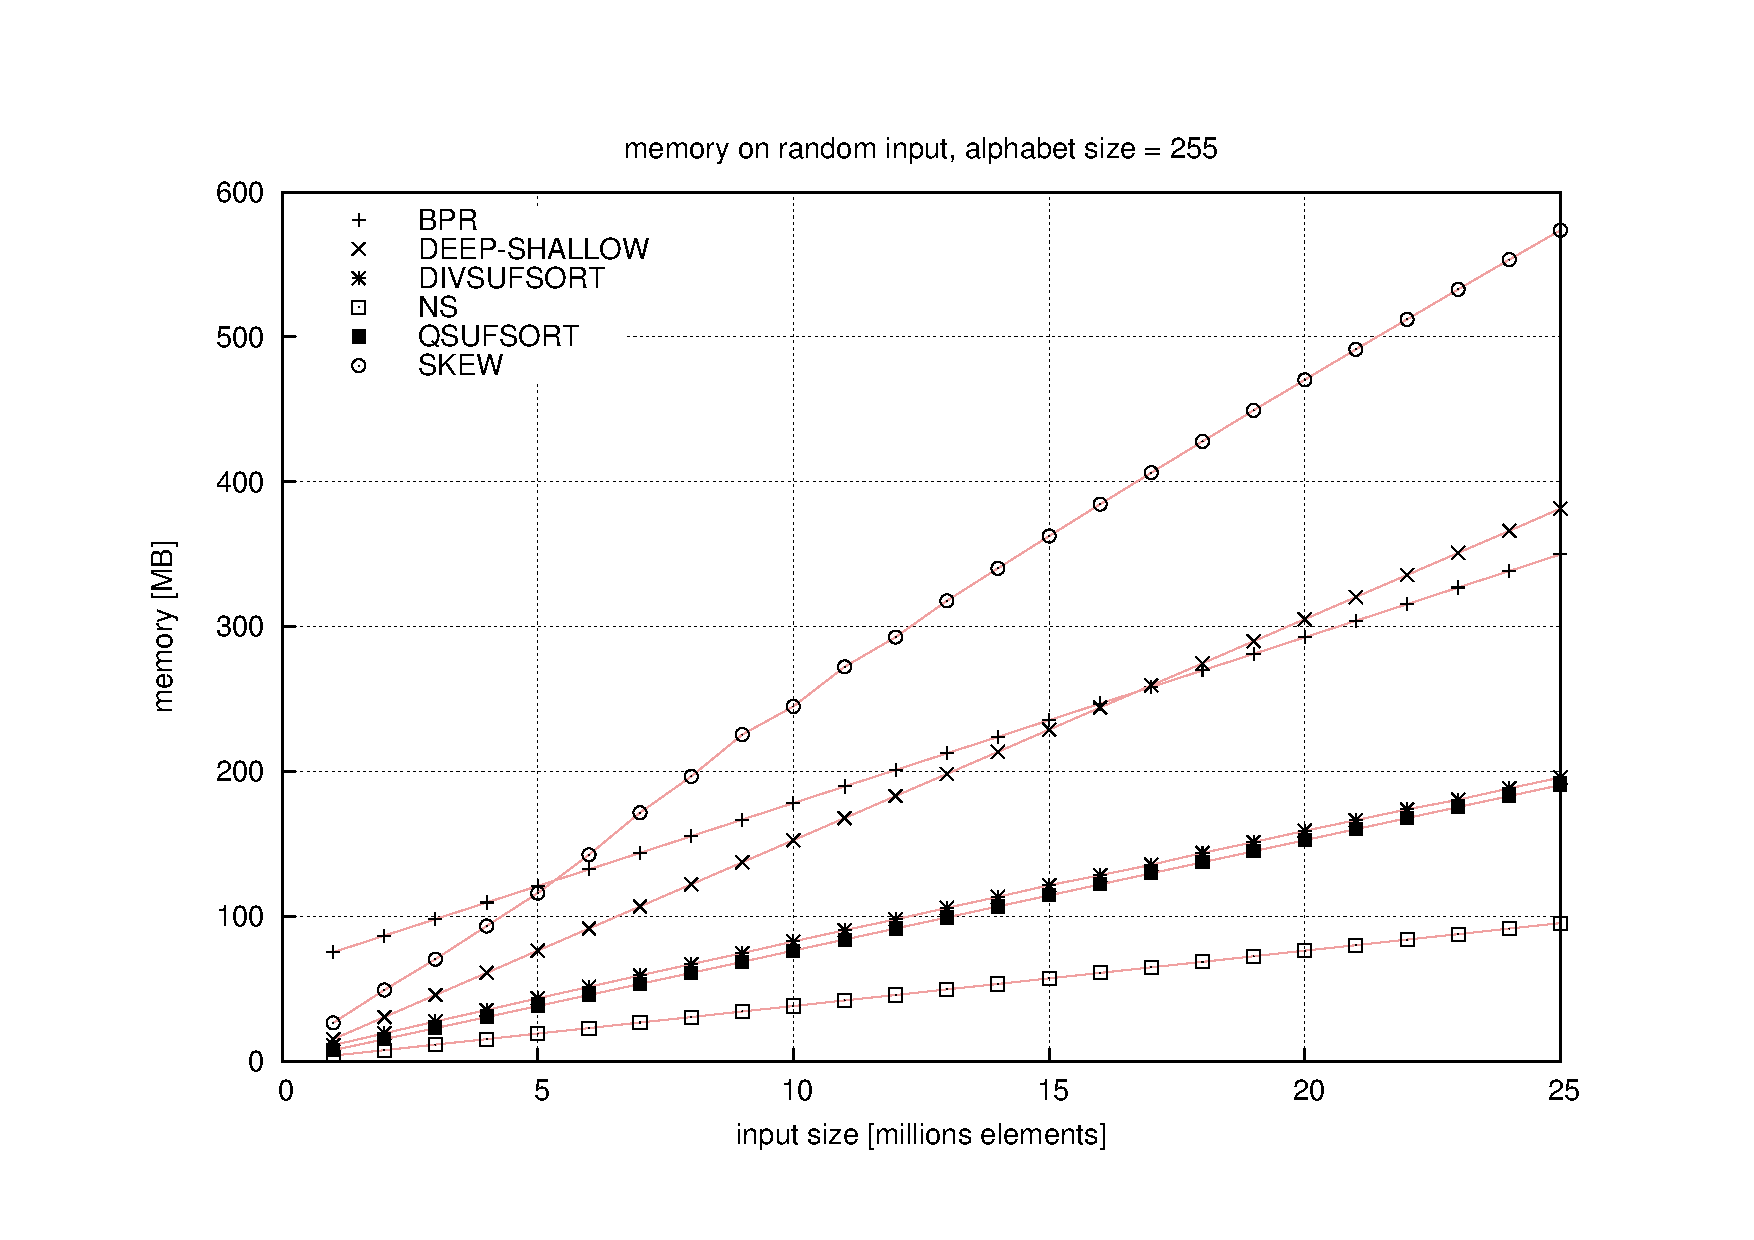
\includegraphics[width=\linewidth]{figures/results/random-input-memory-255.pdf}
        \end{center}        
    \caption{Zużycie pamięci w~zależności od długości wejścia generowanego z~alfabetu wielkości 255.}%
    \label{rys:random-input-memory-255}
\end{figure}

\begin{figure}[tp]
       \begin{center}
            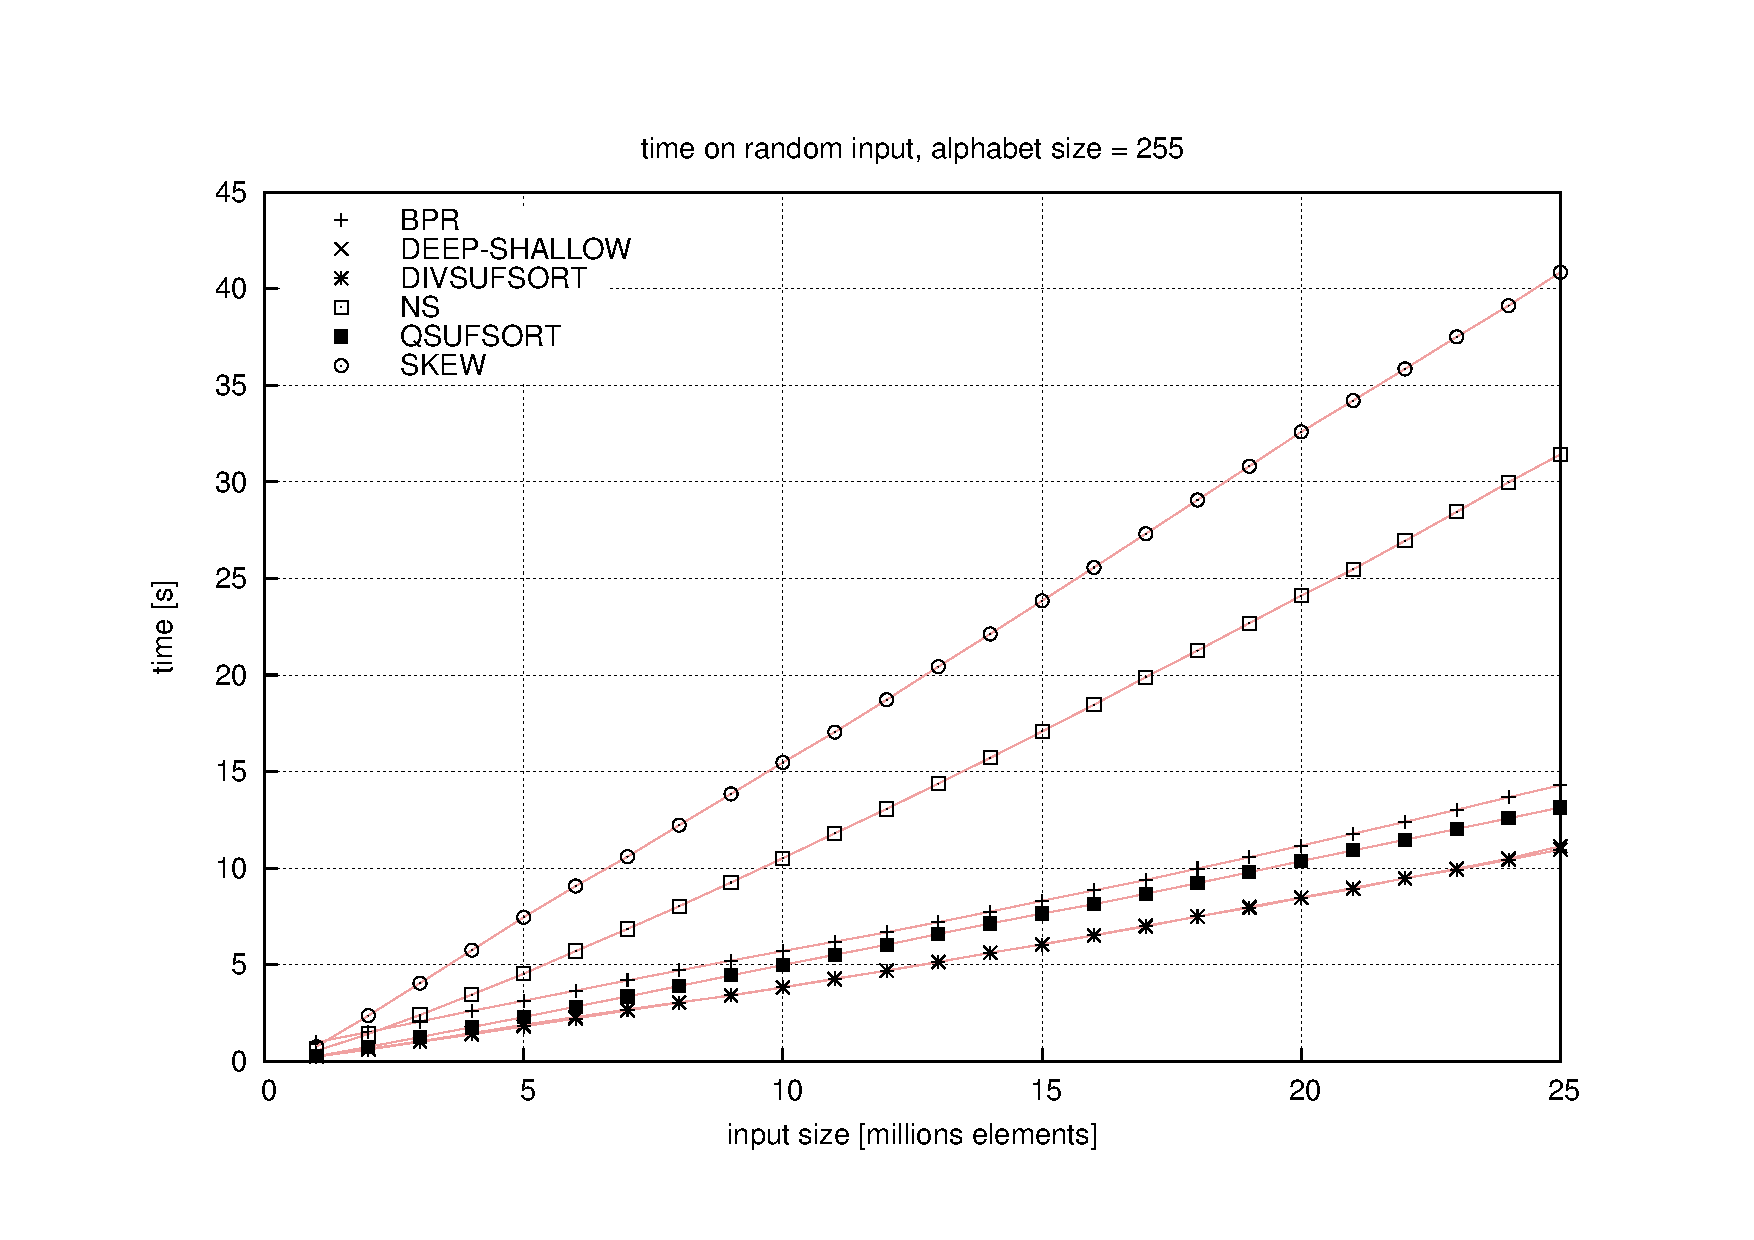
\includegraphics[width=\linewidth]{figures/results/random-input-time-255.pdf}
        \end{center}        
    \caption{Czas działania algorytmów w~zależności od długości wejścia generowanego z~alfabetu wielkości 255.}%
    \label{rys:random-input-time-255}
\end{figure} 


\subsection{Wejście o~stałej długości i~zmiennej wielkości alfabetu}

Wejście generowane na potrzeby testu miało długość 5\,000\,000 elementów. Wykres
\ref{rys:random-alphabet-lcp} przedstawia średnie \emph{lcp} wygenerowanego wejścia w~zależności od
wielkości alfabetu. Wykres \ref{rys:random-alphabet-time} przedstawia czasy działania algorytmów na
generowanym wejściu.

Wyniki testu pokazują które algorytmy zależą od średniego \emph{lcp} i~wielkości alfabetu sekwencji
wejściowej. Algorytm \emph{bpr} jest tego najlepszym przykładem -- im większa jest jedna z~tych
wartości, tym gorzej sobie radzi. Algorytm \emph{skew} uzyskuje lepsze wyniki dla sekwencji
o~większej wartości średniego \emph{lcp}. Pozostałe algorytmy nie wykazują większej zależności
pomiędzy czasem ich działania a~wielkością alfabetu i~średnim \emph{lcp}.
		
\begin{figure}[p]
       \begin{center}
            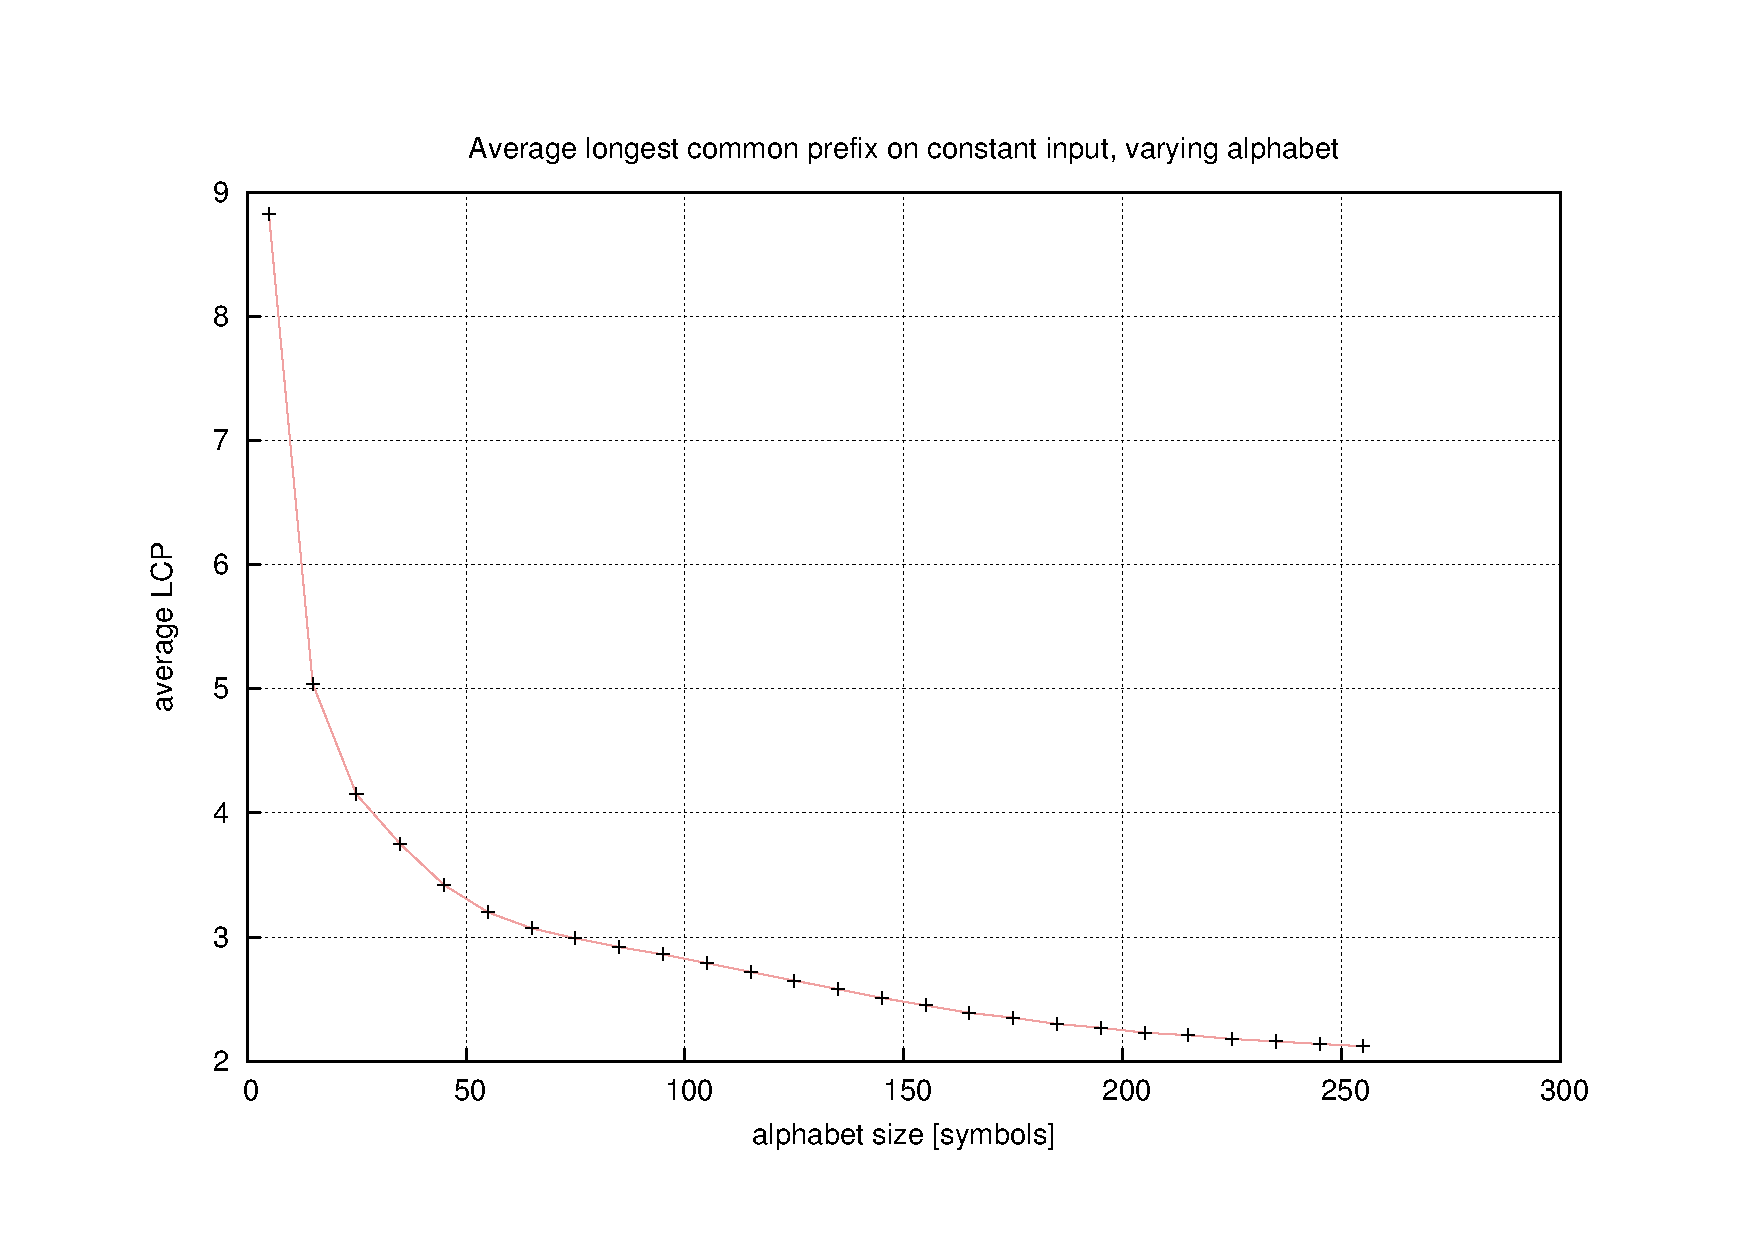
\includegraphics[width=\linewidth]{figures/results/random-alphabet-lcp.pdf}
        \end{center}        
    \caption{Średnie \emph{lcp} generowanego wejścia w~zależności od wielkości alfabetu.}%
    \label{rys:random-alphabet-lcp}
\end{figure}

\begin{figure}[p]
       \begin{center}
            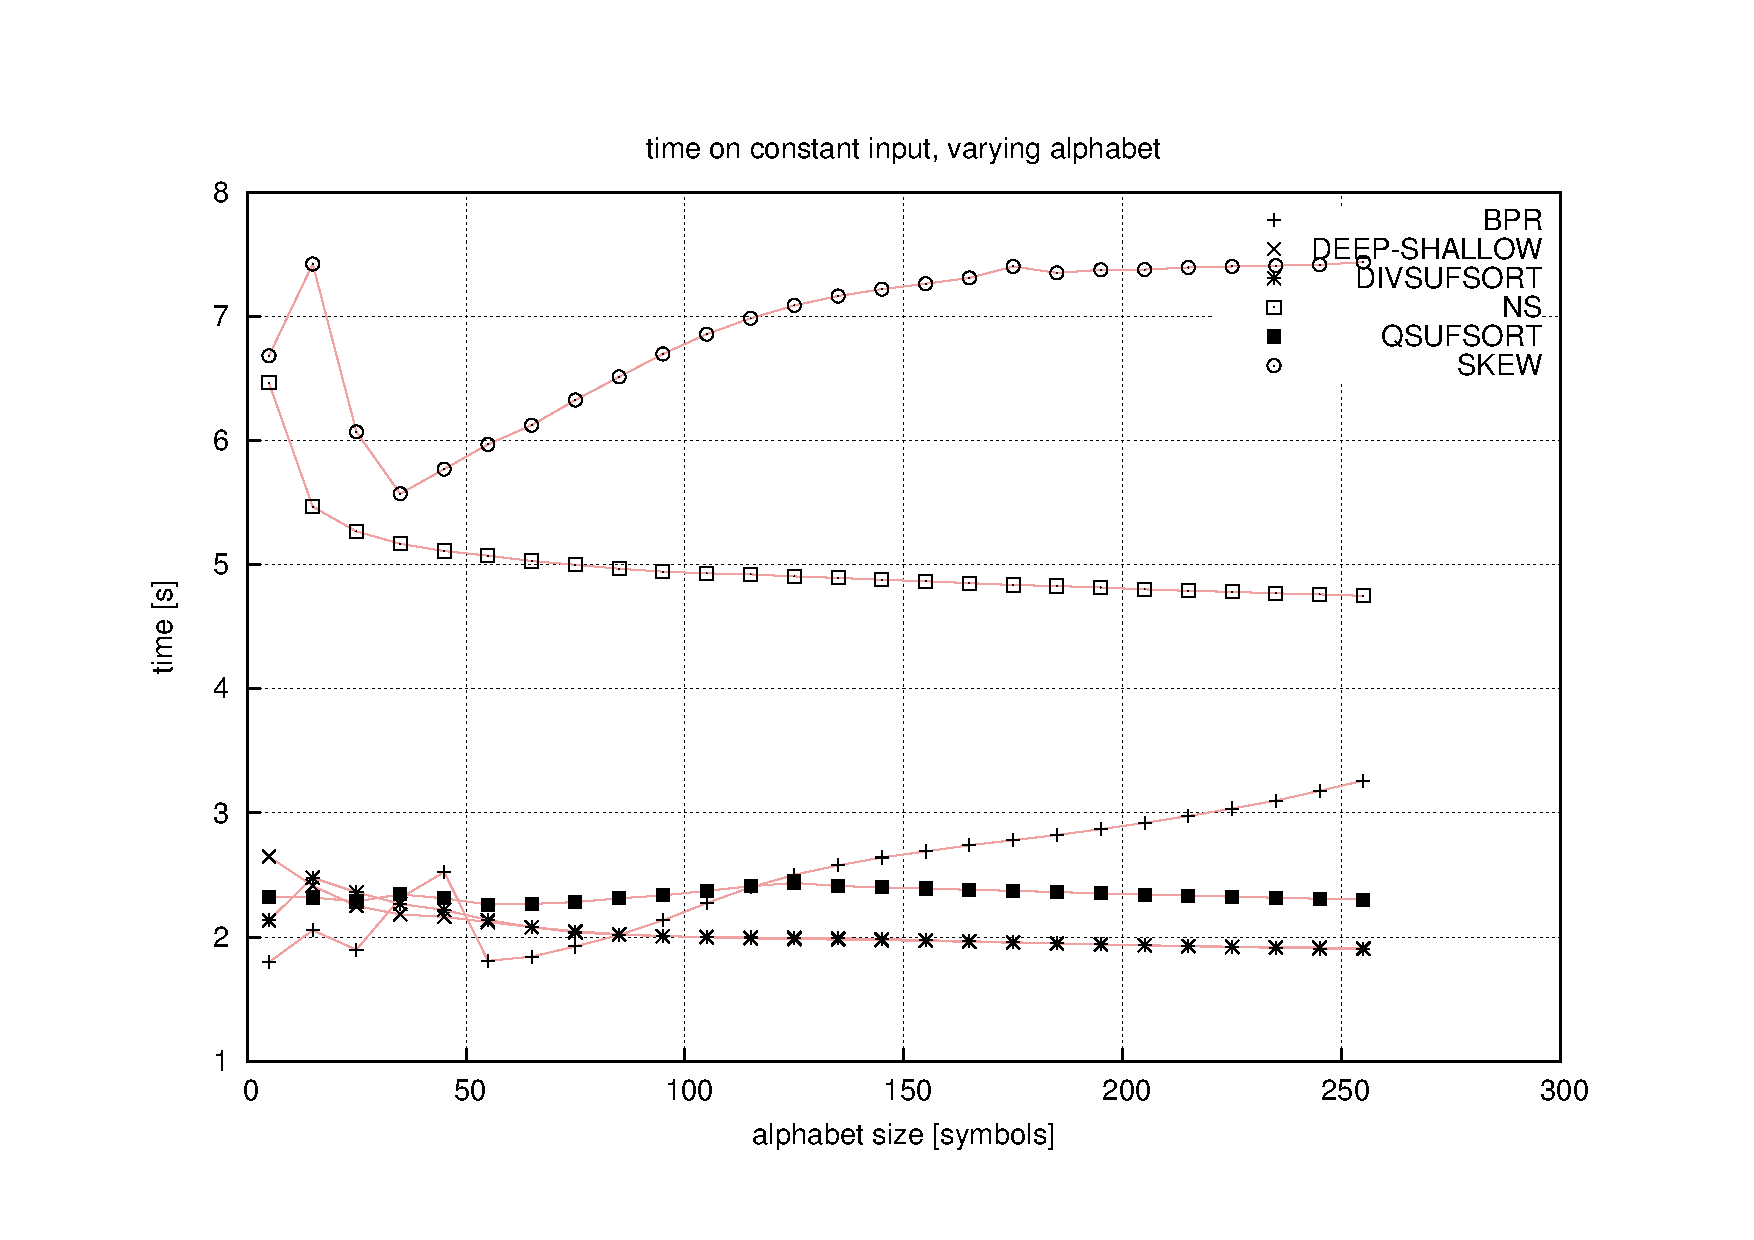
\includegraphics[width=\linewidth]{figures/results/random-alphabet-time.pdf}
        \end{center}        
    \caption{Czas działania algorytmów w~zależności od wielkości alfabetu.}%
    \label{rys:random-alphabet-time}
\end{figure}


% Flush manually before the main section.
\FloatBarrier

\section{Testy wydajnościowe na wejściu wczytywanym z~plików}

Zaimplementowane algorytmy przetestowane zostały na dwóch zestawach plików (korpusach) specjalnie
przygotowanych do testowania algorytmów tworzenia tablic sufiksów. Pierwszy z~nich nosi nazwę
\texttt{Gauntlet}, powstał z~inicjatywy Michaela Maniscalco. Ideą stojącą za stworzeniem tego
korpusu było zebranie plików o~nietypowej strukturze w~celu testowania algorytmów na szczególnych
przypadkach wejścia. Wkład w~powstanie tego zbioru plików wnieśli Yuta Mori, Simon Puglisi oraz
Graham Houston. Korpus dostępny jest do pobrania pod adresem [\ref{gauntlet}].

Drugi korpus testowy opracowany został przez Giovanniego Manziniego. W~jego skład wchodzą
rzeczywiste pliki o~dużym rozmiarze pochodzące z~różnych źródeł. Zestaw plików dostępny jest do
pobrania pod adresem [\ref{manzini-corpus}]. Tabela \ref{tab:manzini-files} prezentuje
charakterystykę plików obu korpusów.

\begin{table}[ht]
    \begin{center} \small
    \begin{tabular}{l r r}
    \toprule
    Plik                    & Rozmiar           & Średnie \emph{lcp} \\ \midrule
    \texttt{abac}           &          200\,000 &         99\,997 \\         
    \texttt{abba}           &      10\,500\,600 &     2\,773\,939 \\         
    \texttt{book1x20}       &      15\,375\,420 &     6\,938\,159 \\         
    \texttt{fib\_s14930352} &      14\,930\,352 &     3\,940\,597 \\         
    \texttt{fss10}          &      12\,078\,908 &     2\,454\,179 \\         
    \texttt{fss9}           &       2\,851\,443 &        579\,353 \\         
    \texttt{houston}        &       3\,840\,000 &         52\,083 \\         
    \texttt{paper5x80}      &          981\,924 &        239\,421 \\         
    \texttt{test1}          &       2\,097\,152 &     1\,048\,064 \\         
    \texttt{test2}          &       2\,097\,152 &     1\,048\,064 \\         
    \texttt{test3}          &       2\,097\,152 &        984\,064 \\         
    \bottomrule
    \end{tabular}
    \hspace{1cm}
    \begin{tabular}{l r r}
    \toprule
    Plik                     & Rozmiar           & Średnie \emph{lcp} \\ \midrule
    \texttt{chr22.dna}       &      34\,553\,758 &          1\,979 \\         
    \texttt{etext99}         &     105\,277\,340 &          1\,108 \\         
    \texttt{gcc-3.0.tar}     &      86\,630\,400 &          8\,603 \\         
    \texttt{howto}           &      39\,422\,105 &             267 \\         
    \texttt{jdk13c}          &      69\,728\,899 &             678 \\         
    \texttt{linux-2.4.5.tar} &     116\,254\,720 &             479 \\         
    \texttt{rctail96}        &     114\,711\,151 &             282 \\         
    \texttt{rfc}             &     116\,421\,901 &              93 \\         
    \texttt{sprot34.dat}     &     109\,617\,186 &              89 \\         
    \texttt{w3c2}            &     104\,201\,579 &         42\,299 \\
    \bottomrule
    \\
    \end{tabular}
    
    \end{center}                         
    \caption{Charakterystyka plików wchodzących w~skład korpusu \texttt{Gauntlet}
    (po lewej) i~korpusu Giovanniego Manziniego (po prawej). Rozmiar i~średnie \emph{lcp} podano w bajtach.}%
    \label{tab:gauntlet-files}\label{tab:manzini-files}
\end{table}


\subsection{Szczegółowe wyniki na maszynie wirtualnej firmy Sun}
    
Ze względu na wysokie podobieństwo wyników, w~poniższym rozdziale prezentowane są szczegółowe
rezultaty tylko z~jednej maszyny wirtualnej (\texttt{sun}). Podobnie jak w~przypadku testów na
różnych komputerach, wyniki testów na różnych maszynach wirtualnych są identyczne w~sensie rankingu
algorytmów.
	
Algorytm \emph{deep-shallow} został pominięty w~poniższych testach ze względu na nieakceptowalnie długi
czas działania. Testy z~jego udziałem wykazały wielokrotnie gorszy czas działania algorytmu od
najgorszego z~pozostałych. Również ze względu na czas działania algorytmu pominięto metodę naiwną.
Algorytmy \emph{skew} i~\emph{bpr} podczas przetwarzania niektórych plików kończyły się wyjątkiem
braku pamięci. Takie przypadki oznaczone zostały w~zestawieniach znakiem --, błąd
działania algorytmu na jednym z~plików danego korpusu powodował pominięcie tej metody w~podsumowaniu
testów na całym zbiorze plików.
	
Wyniki testów na korpusie \texttt{The Gauntlet} przedstawione zostały w~tabeli
\ref{tab:sun-gauntlet}. Rysunek \ref{rys:sun-gauntlet} obrazuje porównanie sumy czasów działania
algorytmów na wszystkich plikach korpusu (poza tymi algorytmami, które błędnie zakończyły
działanie). Analogiczne wyniki testów na korpusie Giovanniego Manziniego przedstawione są w~tabeli
\ref{tab:sun-manzini} oraz rysunku \ref{rys:sun-manzini}. Najlepszym algorytmem okazał się być
\emph{qsufsort}, który uzyskał najlepszy wynik na znakomitej większości plików. Drugie miejsce
przypadło algorytmowi \emph{divsufsort}. Pozostałe algorytmy uzyskiwały znacznie gorsze wyniki lub
nie kończyły obliczeń.


\begin{table}[ht]
    \begin{center}        
        \begin{tabular}{l r r r r } \toprule
 & \emph{bpr} & \emph{divsufsort} & \emph{qsufsort} & \emph{skew}\\ \midrule
\texttt{abac} & 1.83 & 0.05 & \textbf{0.03} & 0.06\\
\texttt{abba} & 4.41 & \textbf{2.82} & 2.85 & 11.62\\
\texttt{book1x20} & \textbf{3.85} & 4.36 & 4.24 & 23.35\\
\texttt{fib\_s14930352} & 11.77 & 6.18 & \textbf{4.15} & 15.18\\
\texttt{fss10} & 6.50 & 4.87 & \textbf{3.04} & 12.26\\
\texttt{fss9} & 1.31 & 0.80 & \textbf{0.69} & 2.32\\
\texttt{houston} & 4.05 & \textbf{0.23} & 0.53 & 1.45\\
\texttt{paper5x80} & 0.19 & 0.15 & \textbf{0.07} & 0.53\\
\texttt{test1} & 3.14 & 0.49 & \textbf{0.25} & 2.27\\
\texttt{test2} & 0.96 & 0.36 & \textbf{0.23} & 2.28\\
\texttt{test3} & 88.37 & 0.54 & \textbf{0.42} & 1.22\\
 \midrule
Total & 126.39 & 20.85 & \textbf{16.51} & 72.53\\
 \bottomrule
\end{tabular}

    \end{center}                         
    \caption{Czas działania algorytmów na plikach z~korpusu \texttt{Gauntlet}.}%
    \label{tab:sun-gauntlet}
\end{table}

\begin{figure}[ht]
   \begin{center}
        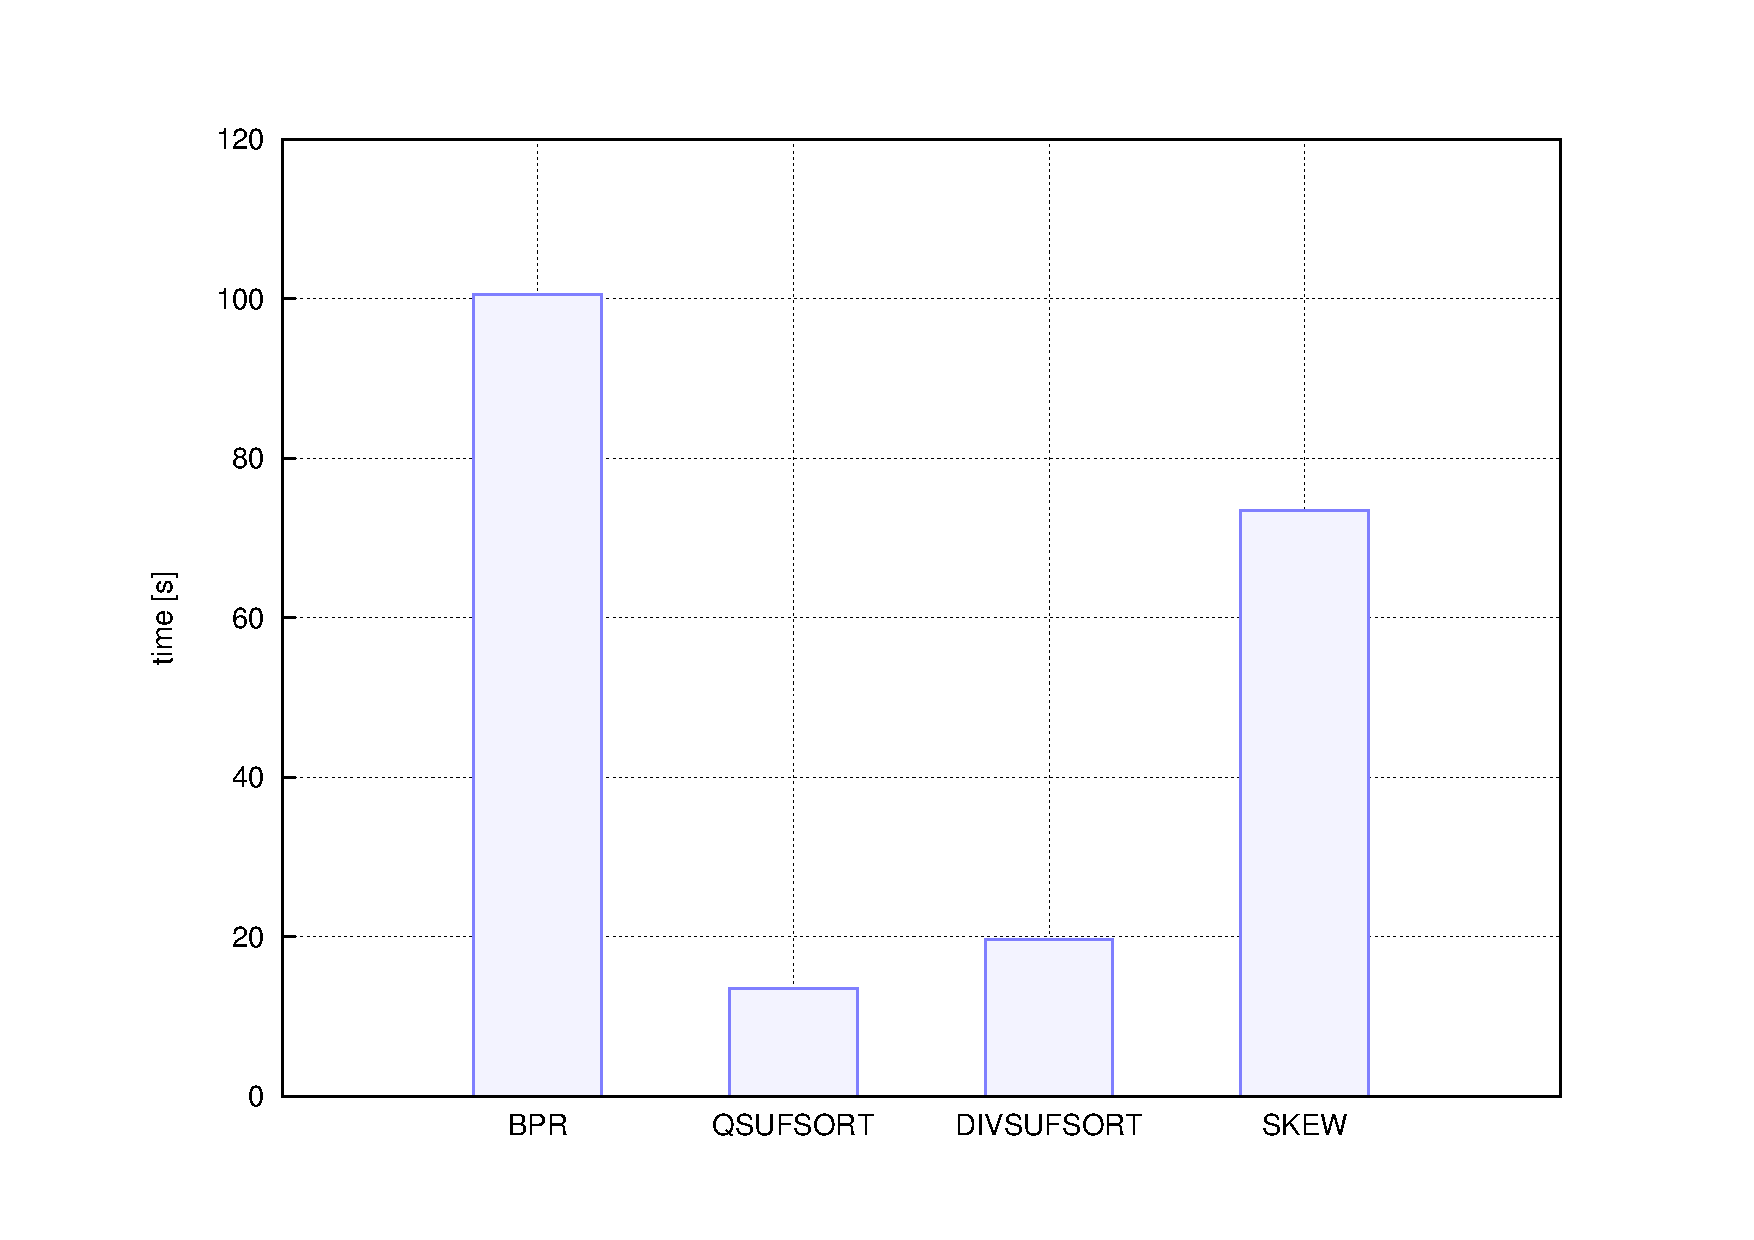
\includegraphics[width=\linewidth]{figures/results/sun-gauntlet.pdf}
    \end{center}        
    \caption{Sumaryczny czas działania algorytmów na plikach z~korpusu \texttt{Gauntlet}.}%
    \label{rys:sun-gauntlet}
\end{figure} 

\begin{table}[ht]
    \begin{center}        
        \begin{tabular}{l r r r r } \toprule
 & \emph{bpr} & \emph{divsufsort} & \emph{qsufsort} & \emph{skew}\\ \midrule
\texttt{chr22.dna} & \textbf{7.31} & 8.54 & 8.15 & 60.73\\
\texttt{etext99} & 28.21 & 29.20 & \textbf{26.35} & ---\\
\texttt{gcc-3.0.tar} & --- & 17.25 & \textbf{14.81} & ---\\
\texttt{howto} & 8.44 & 10.33 & \textbf{7.94} & 79.66\\
\texttt{jdk13c} & 16.44 & 14.74 & \textbf{12.36} & ---\\
\texttt{linux-2.4.5.tar} & 25.60 & 24.09 & \textbf{20.30} & ---\\
\texttt{rctail96} & 30.55 & 28.08 & \textbf{24.60} & ---\\
\texttt{rfc} & 28.93 & 25.92 & \textbf{24.43} & ---\\
\texttt{sprot34.dat} & 28.55 & 28.94 & \textbf{22.89} & ---\\
\texttt{w3c2} & 24.87 & 25.55 & \textbf{17.29} & ---\\
 \midrule
Total &  & 212.62 & \textbf{179.12} & \\
 \bottomrule
\end{tabular}
 
    \end{center}                         
    \caption{Czas działania algorytmów na plikach z~korpusu Giovanniego Manziniego.}%
    \label{tab:sun-manzini}
\end{table}

\begin{figure}[ht]
   \begin{center}
        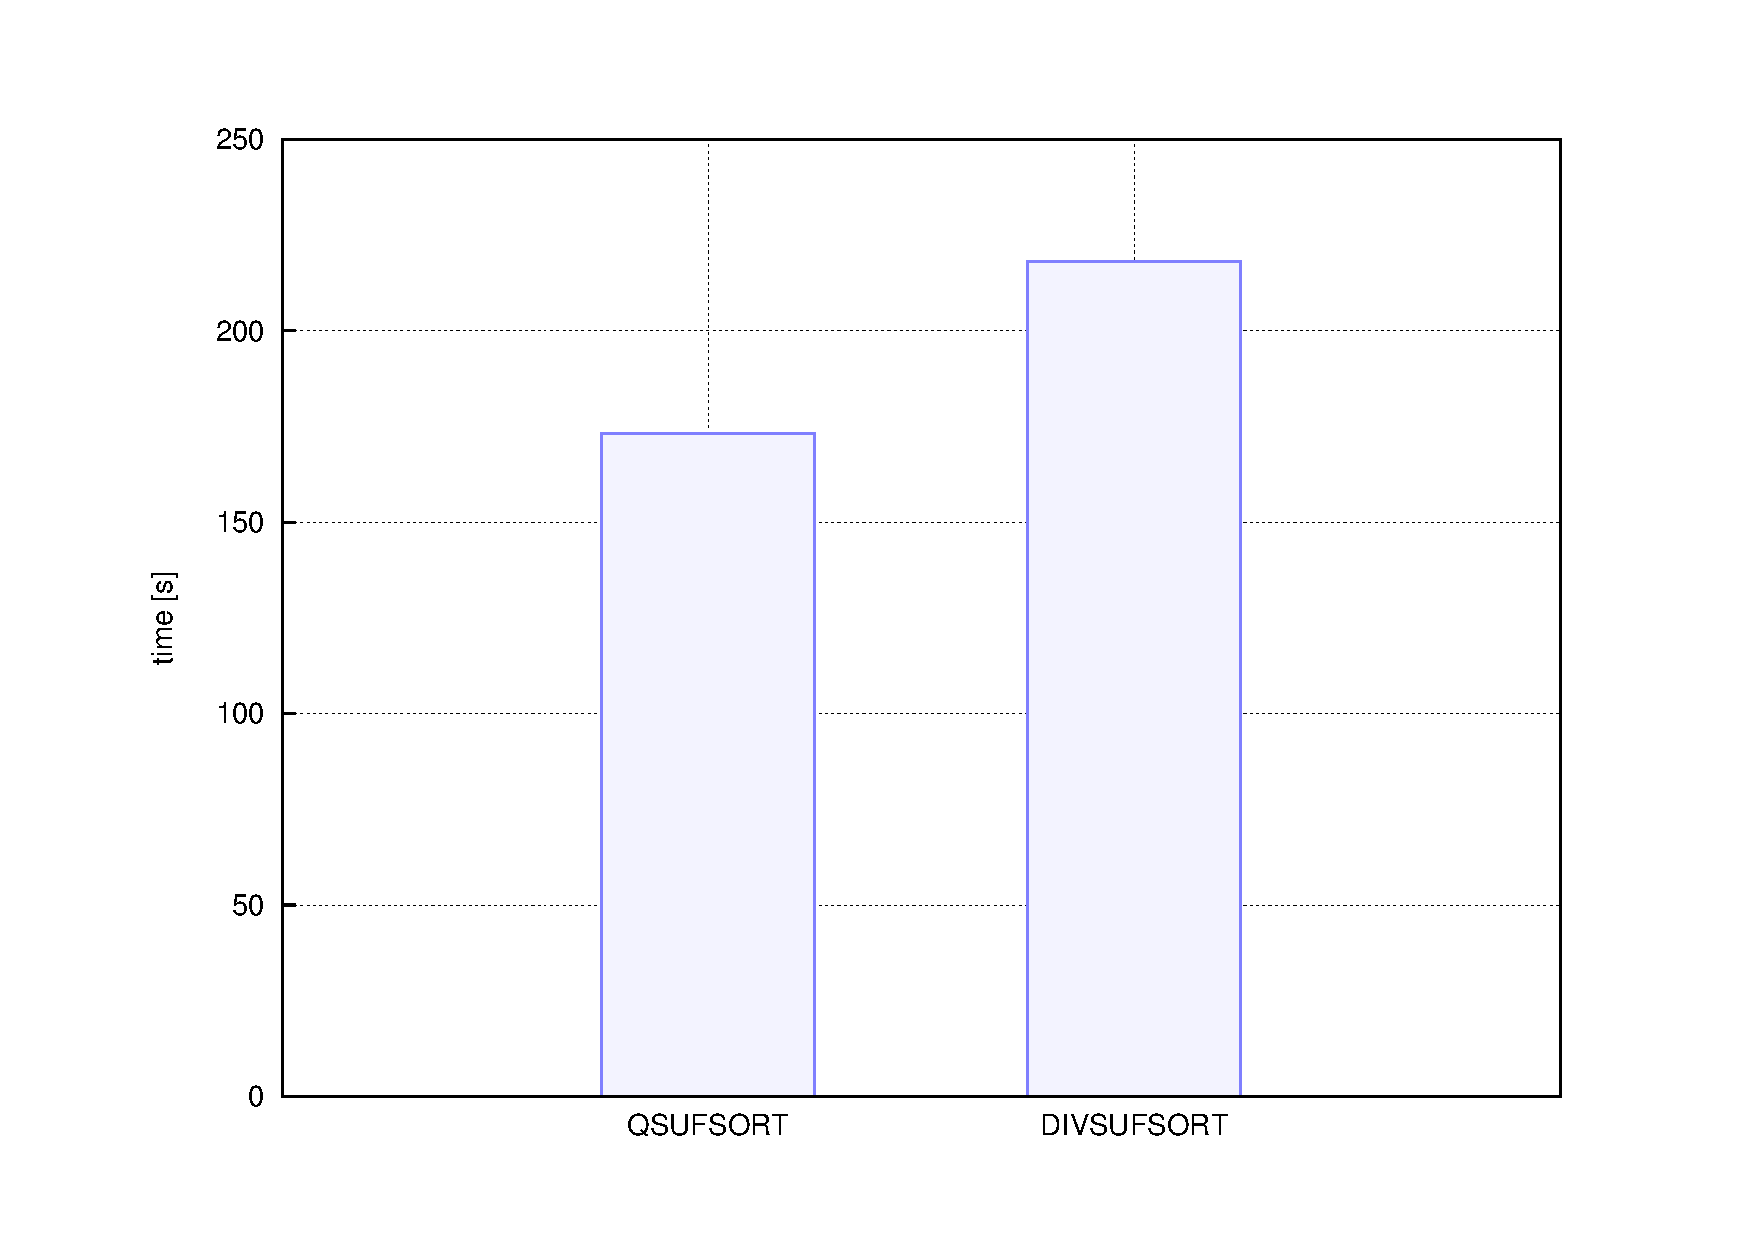
\includegraphics[width=\linewidth]{figures/results/sun-manzini.pdf}
    \end{center}        
    \caption{Sumaryczny czas działania algorytmów na plikach z~korpusu Giovanniego Manziniego.}%
    \label{rys:sun-manzini}
\end{figure} 


\FloatBarrier
\subsection{Porównanie czasów działania algorytmów na różnych maszynach wirtualnych}\label{sect:vms}

Poniżej przedstawione są wyniki podsumowań czasów działania algorytmów na korpusach testowych. Jak
już wspomniano wcześniej, ranking algorytmów jest identyczny dla każdej maszyny wirtualnej. Celem
prezentowania zestawień jest znalezienie takiej maszyny wirtualnej, na której algorytmy działają
najszybciej. Tabele \ref{tab:manzini-vm-compare} i~\ref{tab:gauntlet-vm-compare} zawierają czasy
działań algorytmów na plikach z~korpusów Giovanniego Manziniego i~\texttt{The Gauntlet}. Ze względu
na bardzo niskie wartości odchylenia standardowego nie umieszczono go tabelach. Wizualne porównanie
sum tych wyników znajduje się na rysunkach \ref{rys:manzini-vm-compare}
i~\ref{rys:gauntlet-vm-compare}.
	
Testowane maszyny wirtualne wypadły bardzo podobnie. Na maszynie \texttt{harmony} algorytmy działały
wolniej, wyniki pozostałych trzech maszyn są do siebie zbliżone. Spośród tych wyników wyróżnia się
jednak wynik testu algorytmu \emph{divsufsort} na korpusie Manziniego przeprowadzonego na maszynie
wirtualnej \texttt{jrockit} -- dwukrotnie gorszy niż na pozostałych maszynach. Wyniki w~tabeli
\ref{tab:jrockit-manzini} pokazują wolniejsze działania algorytmu na każdym z~plików wejściowych.
Analiza zapisów przebiegu działania algorytmu wykazała bardzo duże odchylenie standardowe czasu
działania algorytmu, co sugeruje wpływ maszyny wirtualnej (\emph{JIT}, \emph{garbage
collector}) lub jakiś inny proces obliczeniowy działające w tle i~zaburzający pomiar czasu.

\begin{table}[ht]
    \begin{center}        
        \begin{tabular}{l r r r r } \toprule
 & \emph{bpr} & \emph{divsufsort} & \emph{qsufsort} & \emph{skew} \\ \midrule
\texttt{sun} & 100.58 & 19.70 & 13.55 & 73.44 \\
\texttt{ibm} & --- & 18.49 & 14.71 & 71.02 \\
\texttt{jrockit} & 105.05 & 16.49 & 13.55 & 68.24 \\
\texttt{harmony} & 126.39 & 20.85 & 16.51 & 72.53 \\
\bottomrule
\end{tabular}
 
    \end{center}                         
    \caption{Czasy działania algorytmów na korpusie \texttt{Gauntlet} na różnych maszynach wirtualnych. Podane wartości wyrażone są w~sekundach.}
    \label{tab:gauntlet-vm-compare}
\end{table}

\begin{table}[ht]
    \begin{center}        
        \begin{tabular}{l r r r } \toprule
 & \emph{bpr} & \emph{divsufsort} & \emph{qsufsort} \\ \midrule
\texttt{sun} & --- & 218.09 & 173.10  \\
\texttt{ibm} & --- & 212.62 & 179.12 \\
\texttt{jrockit} & 200.84 & 416.30 & 170.00 \\
\texttt{harmony} & 251.82 & 235.16 & 203.76 \\
\bottomrule
\end{tabular}

 
    \end{center}                         
    \caption{Czasy działania algorytmów na korpusie Giovanniego Manziniego na różnych maszynach wirtualnych. Podane wartości wyrażone są w~sekundach.}
    \label{tab:manzini-vm-compare}
\end{table}

% TODO: kolorowe rysunki nie są dobrym pomysłem na wydruk, a te wszystkie kolory są tak samo pastelowe i wyjdą szaro. No
% chyba, że będziesz drukował w kolorze...

\begin{figure}[p]
    \begin{center}
        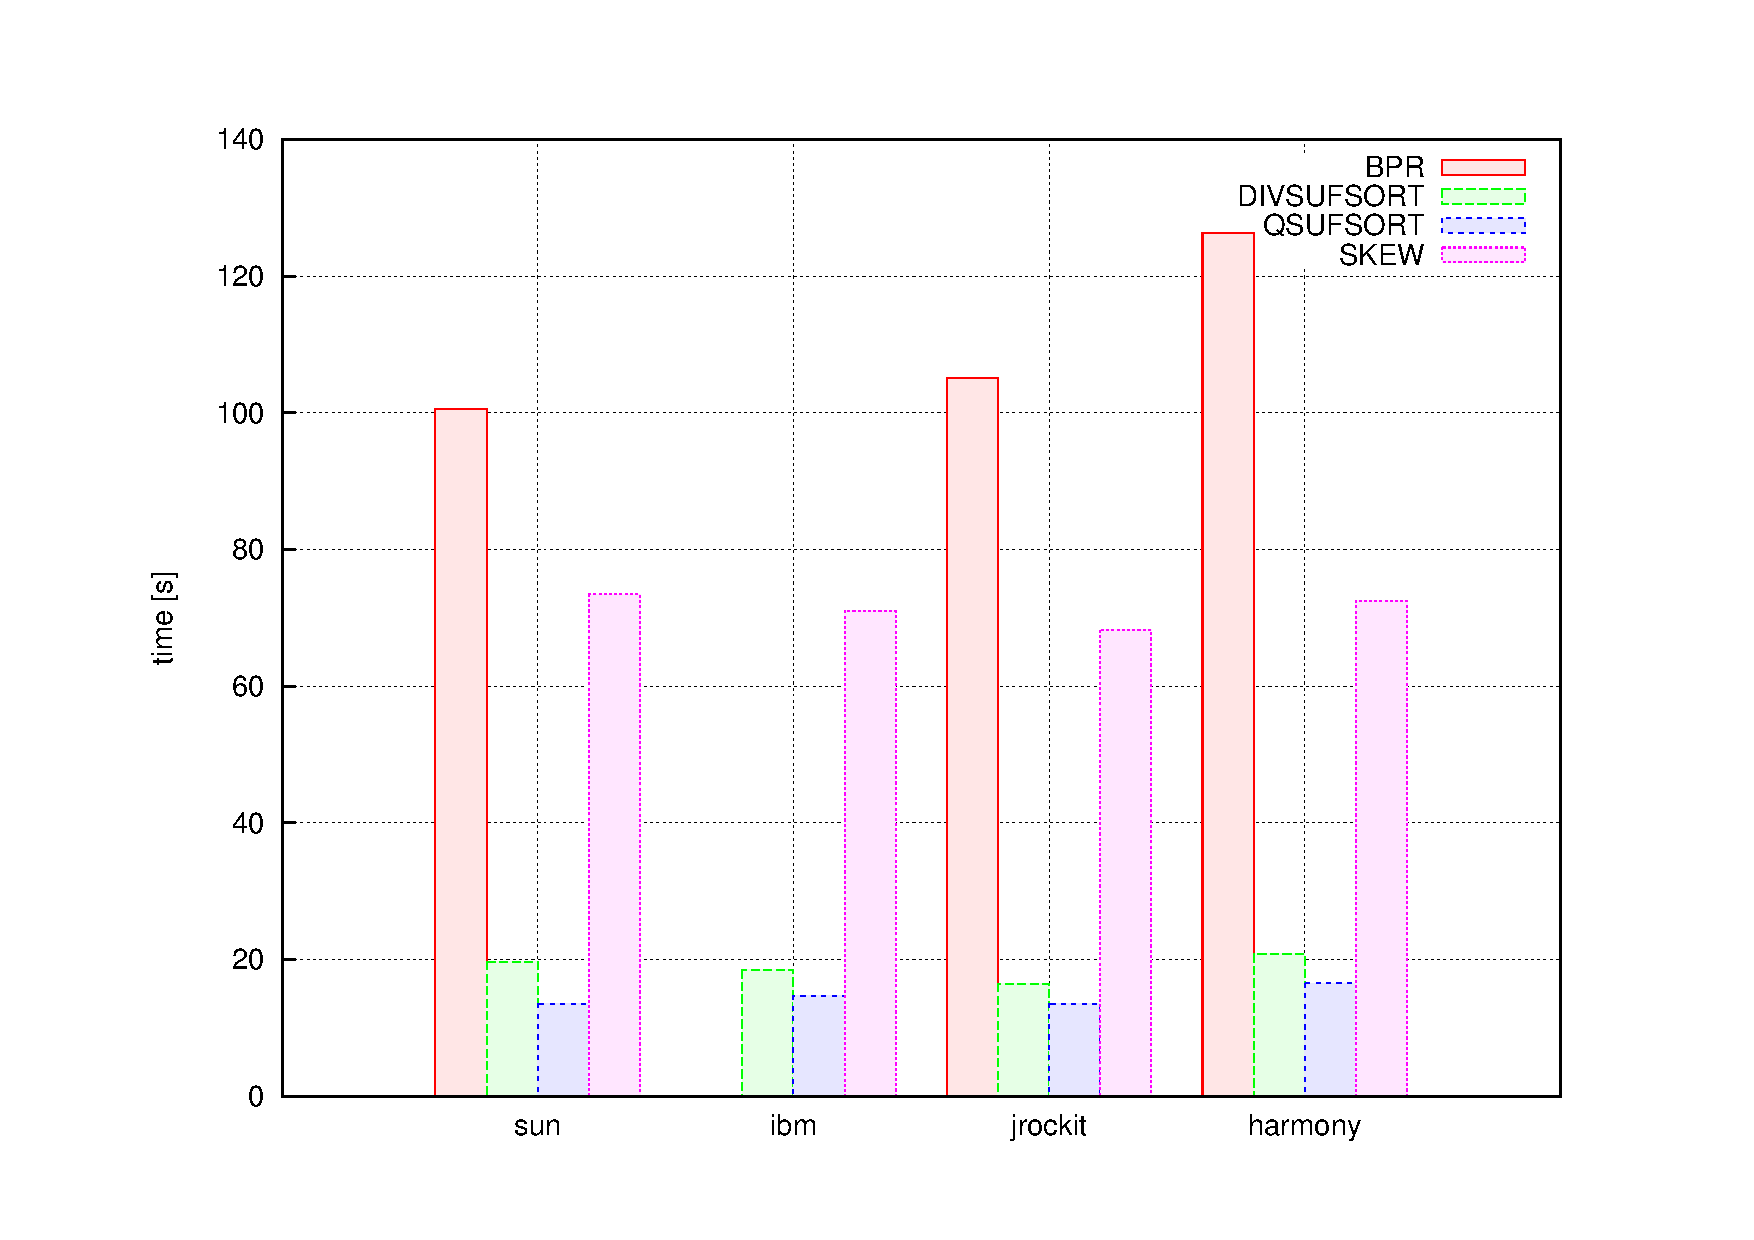
\includegraphics[width=.9\linewidth]{figures/results/gauntlet-compare.pdf}
    \end{center}        
    \caption{Porównanie czasu działania algorytmów na korpusie \texttt{Gauntlet} na różnych maszynach wirtualnych.}
    \label{rys:gauntlet-vm-compare}
\end{figure}

\begin{figure}[p]
    \begin{center}
        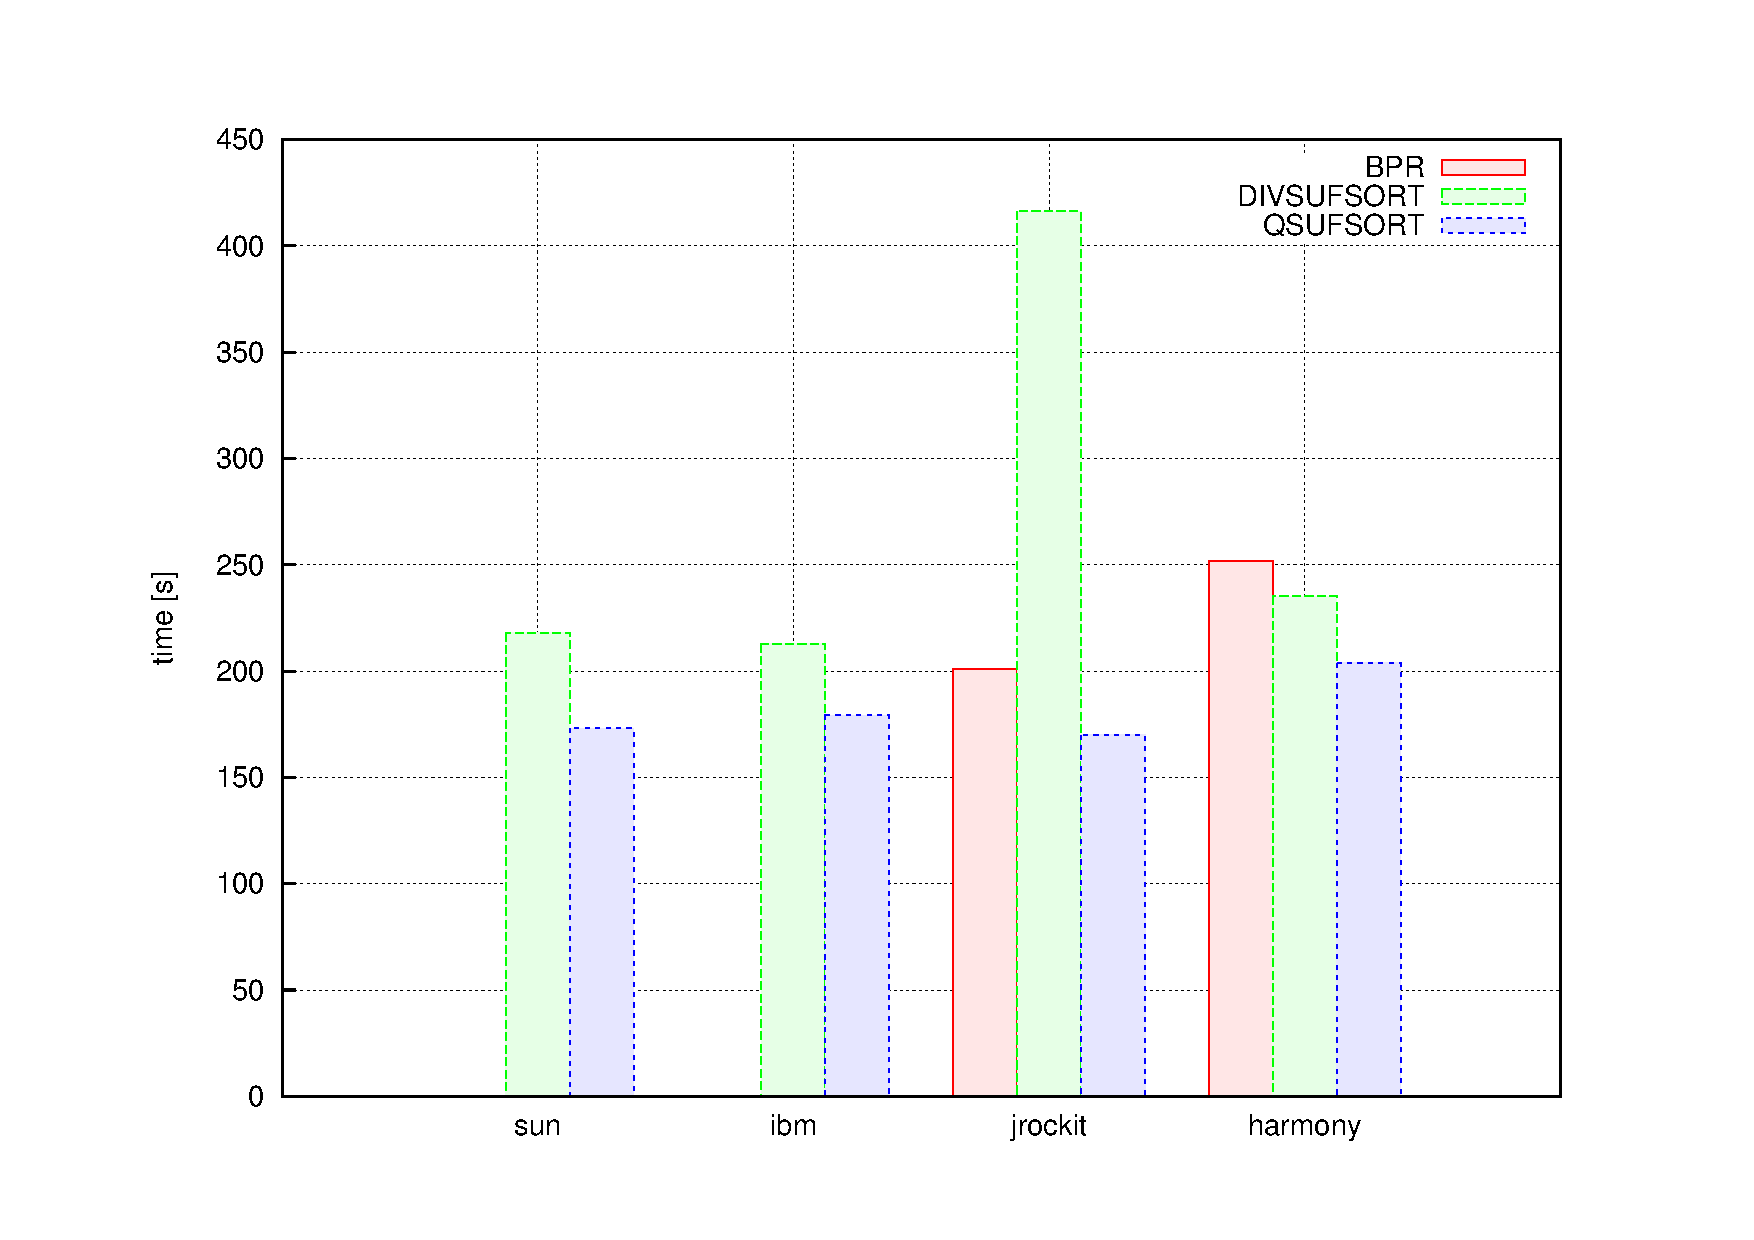
\includegraphics[width=.9\linewidth]{figures/results/manzini-compare.pdf}
        \end{center}        
        \caption{Porównanie czasu działania algorytmów na korpusie Giovanniego Manziniego na różnych maszynach wirtualnych.}
        \label{rys:manzini-vm-compare}
\end{figure}


\FloatBarrier
\section{Analiza wyników}

Najlepszym spośród zaimplementowanych algorytmów okazał się algorytm \emph{qsufsort}. Cechuje się on
odpornością na specyficzne typy danych wejściowych, nie zależy w dużym stopniu ani od rozmiaru
alfabetu sekwencji wejściowej ani od wartości średniego \emph{lcp}. Dodatkowym atutem jest brak
użycia dodatkowej pamięci ponad tą wymaganą do przechowania wejścia i~wyjścia algorytmu (oraz stosu
zużytego podczas rekurencyjnego sortowania). Na drugim miejscu znalazł się algorytm
\emph{divsufsort} ustępujący zwycięzcy zarówno pod względem czasu działania, jak i~zużycia pamięci.
Pozostałe algorytmy wypadły dużo gorzej niż wymieniona dwójka.

Co ciekawe, publikowane w~internecie wyniki testów wydajnościowych implementacji algorytmów w~języku
\texttt{C++} [\ref{msufsort}, \ref{mori-benchmark}] dają nieco inny obraz rankingu tych algorytmów.
Najlepsze wyniki uzyskują tam implementacje algorytmu \emph{improved two-stage}, czyli
\emph{archon}, \emph{divsufsort} i~\emph{msufsort}. Algorytm \emph{qsufsort} uzyskuje dobre, choć
wyraźnie gorsze wyniki. Wytłumaczenie przyczyn tego faktu leży zapewne w~różnicach między językami
\texttt{C++} a~\texttt{Java} (oraz działaniem kodu natywnego i~kodu uruchamianego na maszynie
wirtualnej). Algorytm \emph{qsufsort} jest prostym algorytmem, zarówno koncepcyjnie jak
i~implementacyjnie. Przepisanie go z~\texttt{C++} do \texttt{Javy} nie było trudne. Algorytm
\emph{divsufsort} jest dużo bardziej złożony (jego implementacja w~języku \texttt{Java} jest o~ponad
2000 linii kodu dłuższa od \emph{qsufsort}). Z~powodu wykorzystywania wskaźników oraz instrukcji
\texttt{\#define} w~oryginalnej implementacji, kod w~języku \texttt{Java} różni się od oryginału
w~wielu miejscach. Wydaje się, że dominujące dla szybkości działania różnice to:
\begin{itemize}
    \item allokacja złożonych struktur danych (i tablic lokalnych) następuję w języku \texttt{Java}
    na stercie, a nie na stosie; oprócz samego narzutu allokacji dochodzi tu również koszt 
    procesu oczyszczania pamięci (\emph{garbage collector});
    
    \item wskaźniki z języków niskopoziomowych muszą być modelowane jako indeksy nad tablicami typów prostych, 
    co w języku \texttt{Java} wiąże się z dodatkowym narzutem sprawdzenia czy indeks nie przekracza
    rozmiaru tablicy;

    \item rozmiar kodu natywnego generowanego dynamicznie w języku \texttt{Java} prawdopodobnie przekraczał wielokrotnie
    rozmiar kodu skompilowanego w języku \texttt{C}, powodując gorsze użytkowanie pamięci podręcznej
    procesora.
\end{itemize}

Algorytm \emph{skew} jako jedyny spośród testowanych algorytmów posiadał liniową teoretyczną złożoność
obliczeniową. W~testach wydajnościowych wypadł jednak bardzo słabo, zarówno w~testach implementacji
w~języku \texttt{Java}, jak i~w~języku \texttt{C++}. Przyczyną takiego zachowania algorytmu jest
jego bardzo duża złożoność pamięciowa zwiększana dodatkowo przez rekurencyjne wywoływanie algorytmu.
Ponadto, rekurencja wiąże się z~dodatkowymi kosztami związanymi z~obsługą stosu. Należy również
pamiętać, że podane złożoności pozostałych algorytmów są wartościami pesymistycznymi, które są
rzadko osiągane w praktyce.



\chapter{Podsumowanie i kierunki dalszego rozwoju}




% All appendices and extra material, if you have any.
\cleardoublepage\appendix%

\chapter{Wyniki dla pozostałych maszyn wirtualnych}

\begin{table}[p]
	\begin{center}        
 		\begin{tabular}{l r r r r } \toprule
 & \emph{bpr} & \emph{divsufsort} & \emph{qsufsort} & \emph{skew}\\ \midrule
\texttt{abac} & 1.83 & 0.05 & \textbf{0.03} & 0.06\\
\texttt{abba} & 4.41 & \textbf{2.82} & 2.85 & 11.62\\
\texttt{book1x20} & \textbf{3.85} & 4.36 & 4.24 & 23.35\\
\texttt{fib\_s14930352} & 11.77 & 6.18 & \textbf{4.15} & 15.18\\
\texttt{fss10} & 6.50 & 4.87 & \textbf{3.04} & 12.26\\
\texttt{fss9} & 1.31 & 0.80 & \textbf{0.69} & 2.32\\
\texttt{houston} & 4.05 & \textbf{0.23} & 0.53 & 1.45\\
\texttt{paper5x80} & 0.19 & 0.15 & \textbf{0.07} & 0.53\\
\texttt{test1} & 3.14 & 0.49 & \textbf{0.25} & 2.27\\
\texttt{test2} & 0.96 & 0.36 & \textbf{0.23} & 2.28\\
\texttt{test3} & 88.37 & 0.54 & \textbf{0.42} & 1.22\\
 \midrule
Total & 126.39 & 20.85 & \textbf{16.51} & 72.53\\
 \bottomrule
\end{tabular}

    \end{center}                         
	\caption{Czas działania algorytmów na plikach z korpusu \texttt{The Gauntlet} dla maszyny wirtualnej \texttt{ibm}.}%
    \label{tab:ibm-gauntlet}
\end{table}

\begin{figure}[p]
   \begin{center}
        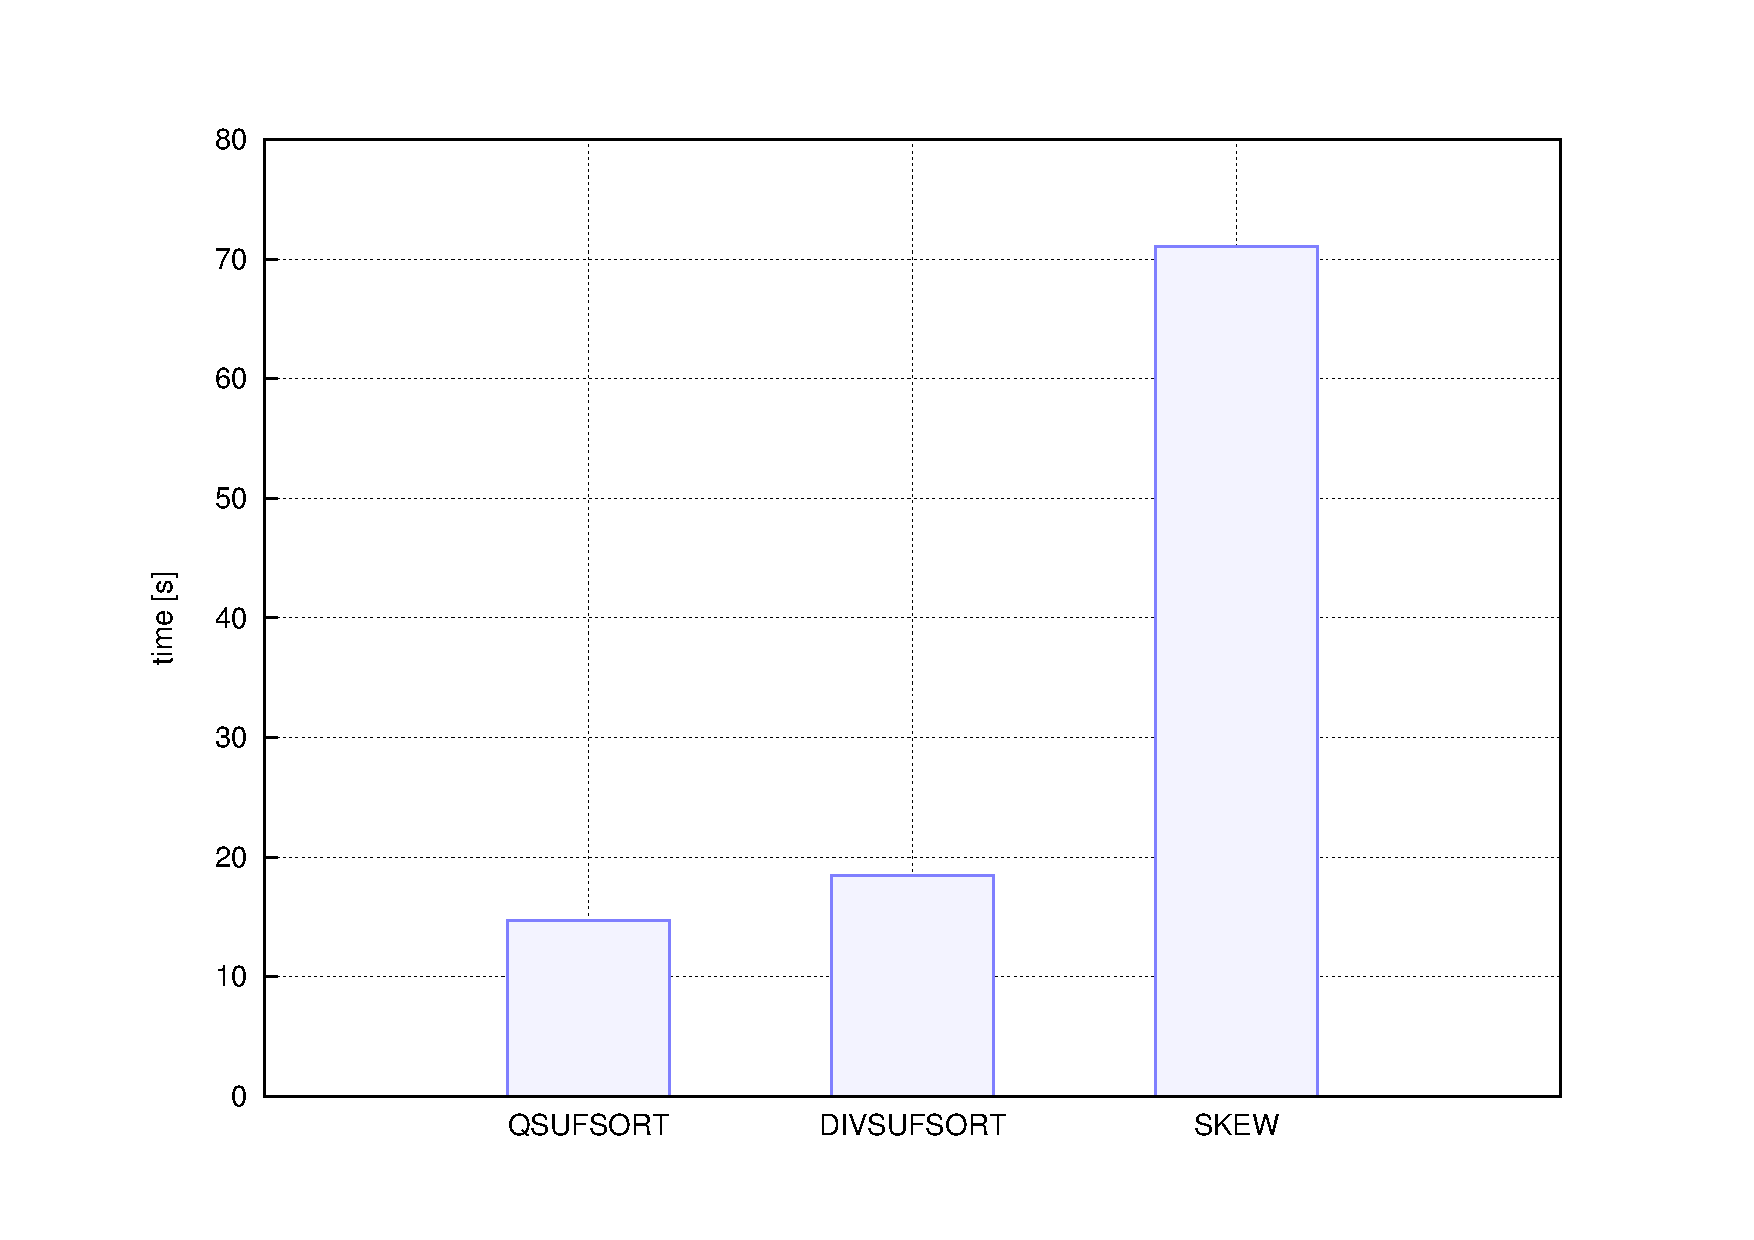
\includegraphics[width=\linewidth]{figures/results/ibm-gauntlet.pdf}
    \end{center}        
    \caption{Sumaryczny czas działania algorytmów na plikach z korpusu \texttt{The Gauntlet} dla maszyny wirtualnej \texttt{ibm}.}%
    \label{rys:ibm-gauntlet}
\end{figure}


\begin{table}[p]
	\begin{center}        
 		\begin{tabular}{l r r r r } \toprule
 & \emph{bpr} & \emph{divsufsort} & \emph{qsufsort} & \emph{skew}\\ \midrule
\texttt{chr22.dna} & \textbf{7.31} & 8.54 & 8.15 & 60.73\\
\texttt{etext99} & 28.21 & 29.20 & \textbf{26.35} & ---\\
\texttt{gcc-3.0.tar} & --- & 17.25 & \textbf{14.81} & ---\\
\texttt{howto} & 8.44 & 10.33 & \textbf{7.94} & 79.66\\
\texttt{jdk13c} & 16.44 & 14.74 & \textbf{12.36} & ---\\
\texttt{linux-2.4.5.tar} & 25.60 & 24.09 & \textbf{20.30} & ---\\
\texttt{rctail96} & 30.55 & 28.08 & \textbf{24.60} & ---\\
\texttt{rfc} & 28.93 & 25.92 & \textbf{24.43} & ---\\
\texttt{sprot34.dat} & 28.55 & 28.94 & \textbf{22.89} & ---\\
\texttt{w3c2} & 24.87 & 25.55 & \textbf{17.29} & ---\\
 \midrule
Total &  & 212.62 & \textbf{179.12} & \\
 \bottomrule
\end{tabular}
 
    \end{center}                         
	\caption{Czas działania algorytmów na plikach z korpusu Giovanniego Manziniego dla maszyny wirtualnej \texttt{ibm}.}%
    \label{tab:ibm-manzini}
\end{table}

\begin{figure}[p]
       \begin{center}
            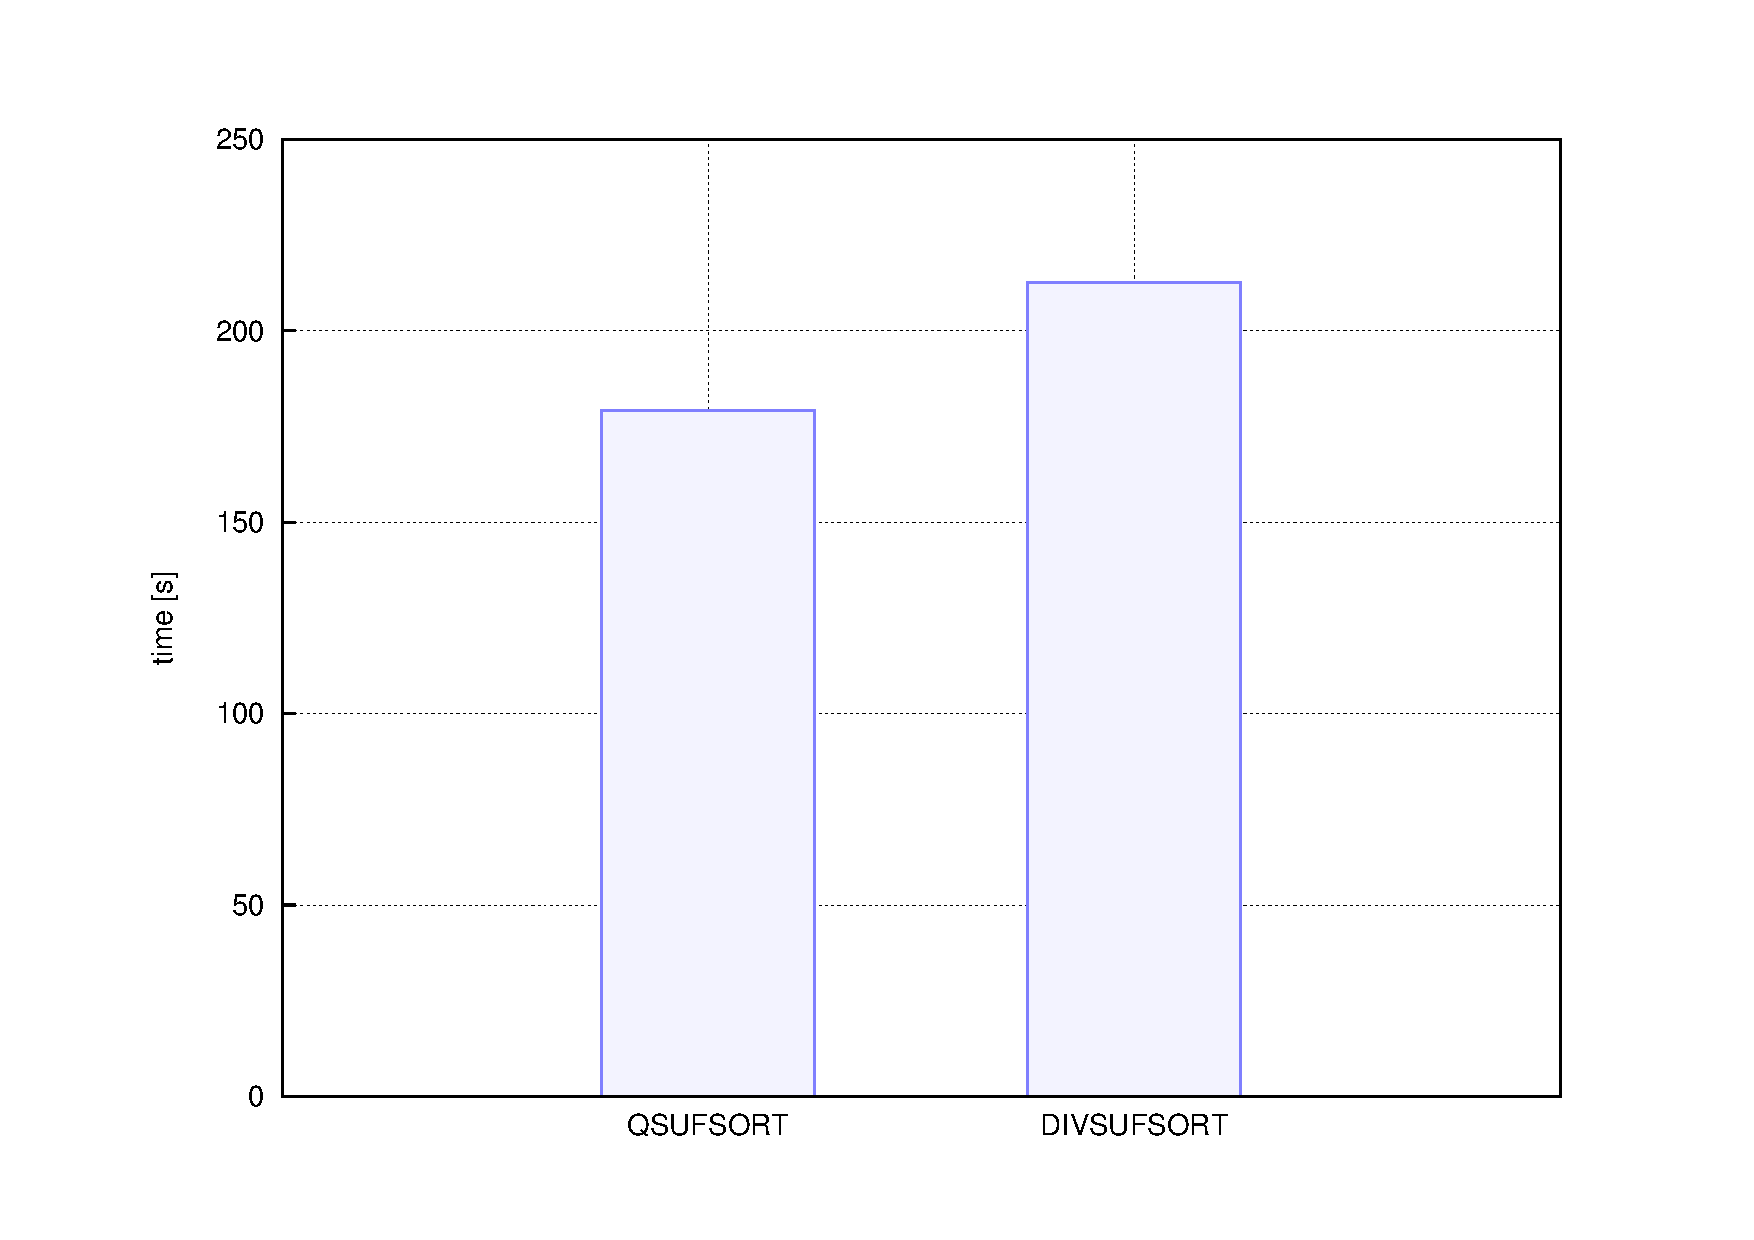
\includegraphics[width=\linewidth]{figures/results/ibm-manzini.pdf}
        \end{center}        
	    \caption{Sumaryczny czas działania algorytmów na plikach z korpusu Giovanniego Manziniego dla maszyny wirtualnej \texttt{ibm}.}%
    \label{rys:ibm-manzini}
\end{figure}
 

\begin{table}[p]
	\begin{center}        
 		\begin{tabular}{l r r r r } \toprule
 & \emph{bpr} & \emph{divsufsort} & \emph{qsufsort} & \emph{skew}\\ \midrule
\texttt{abac} & 1.83 & 0.05 & \textbf{0.03} & 0.06\\
\texttt{abba} & 4.41 & \textbf{2.82} & 2.85 & 11.62\\
\texttt{book1x20} & \textbf{3.85} & 4.36 & 4.24 & 23.35\\
\texttt{fib\_s14930352} & 11.77 & 6.18 & \textbf{4.15} & 15.18\\
\texttt{fss10} & 6.50 & 4.87 & \textbf{3.04} & 12.26\\
\texttt{fss9} & 1.31 & 0.80 & \textbf{0.69} & 2.32\\
\texttt{houston} & 4.05 & \textbf{0.23} & 0.53 & 1.45\\
\texttt{paper5x80} & 0.19 & 0.15 & \textbf{0.07} & 0.53\\
\texttt{test1} & 3.14 & 0.49 & \textbf{0.25} & 2.27\\
\texttt{test2} & 0.96 & 0.36 & \textbf{0.23} & 2.28\\
\texttt{test3} & 88.37 & 0.54 & \textbf{0.42} & 1.22\\
 \midrule
Total & 126.39 & 20.85 & \textbf{16.51} & 72.53\\
 \bottomrule
\end{tabular}

    \end{center}                         
	\caption{Czas działania algorytmów na plikach z korpusu \texttt{The Gauntlet} dla maszyny wirtualnej \texttt{jrockit}.}%
    \label{tab:jrockit-gauntlet}
\end{table}

\begin{figure}[p]
       \begin{center}
            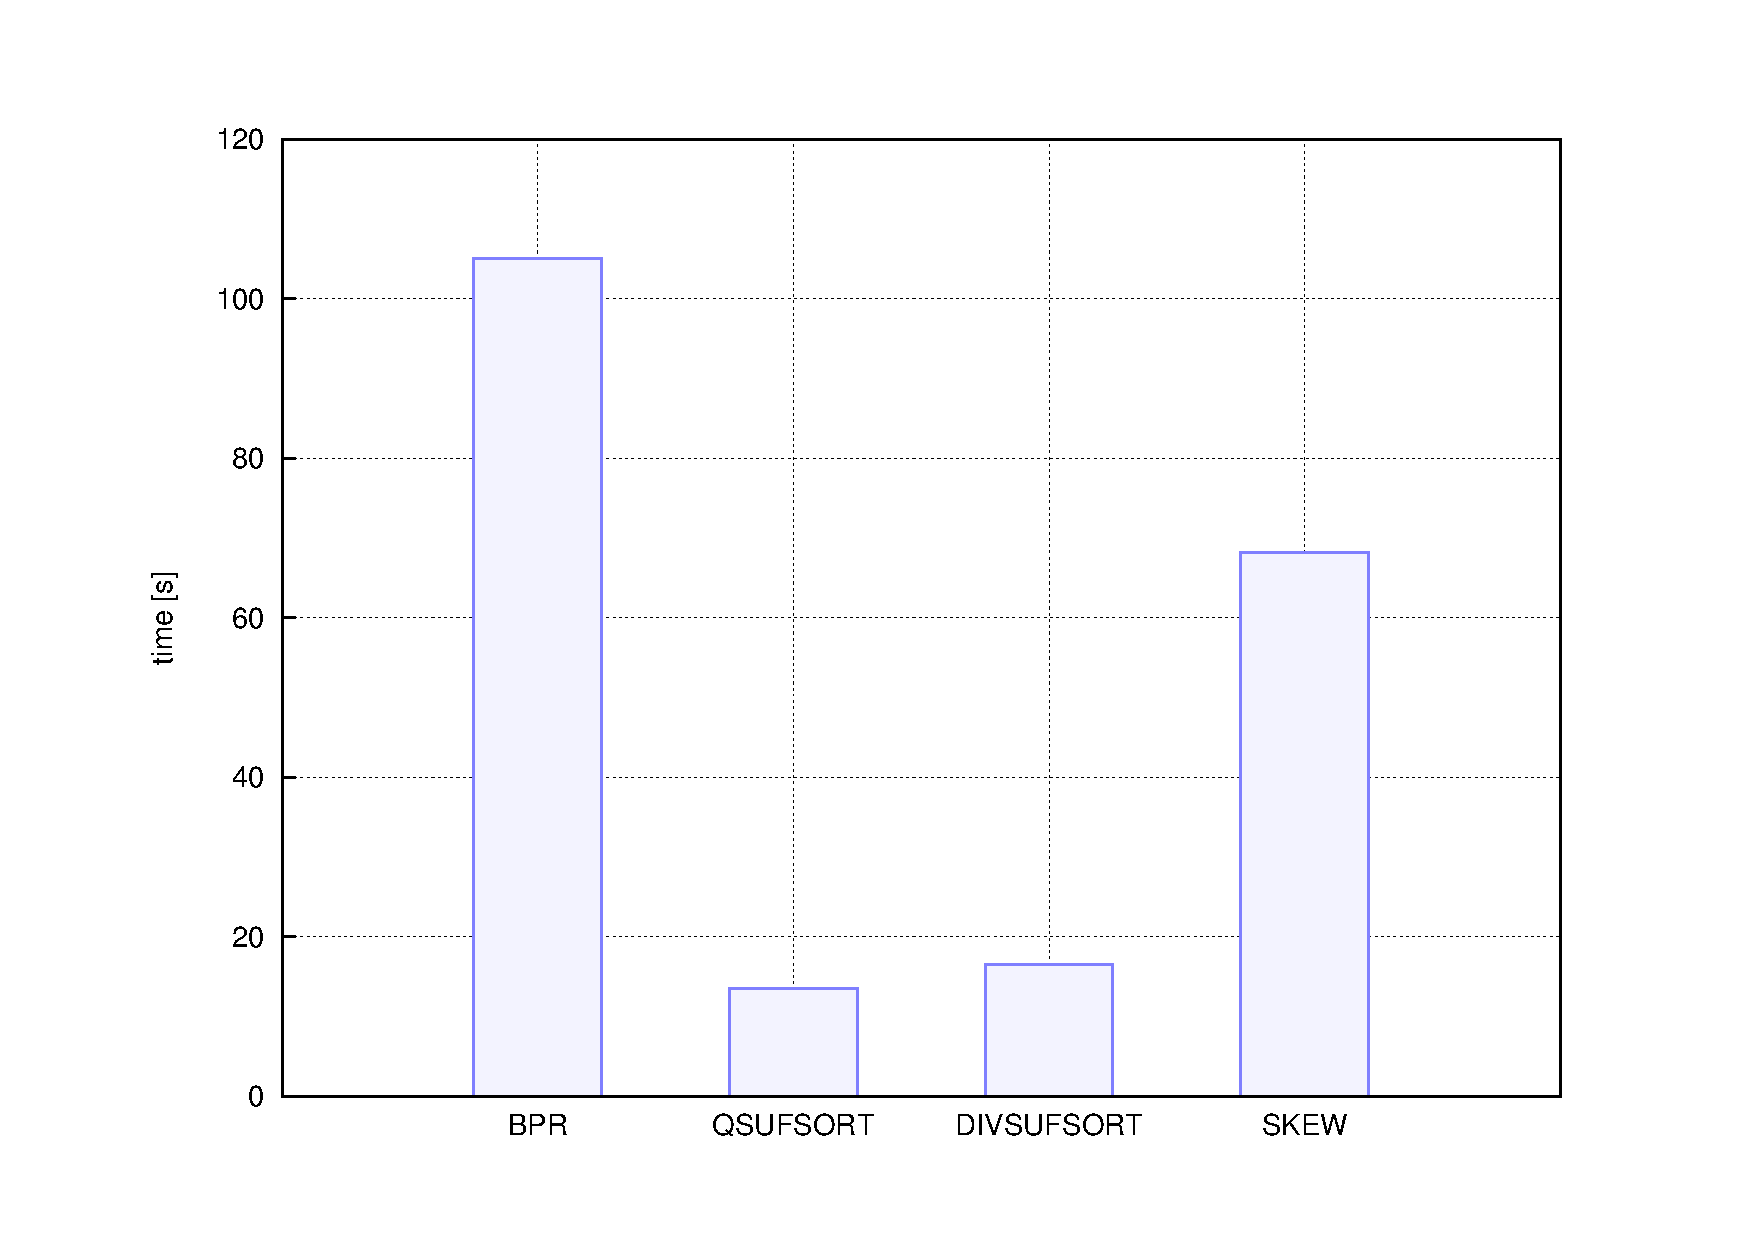
\includegraphics[width=\linewidth]{figures/results/jrockit-gauntlet.pdf}
        \end{center}        
	    \caption{Sumaryczny czas działania algorytmów na plikach z korpusu \texttt{The Gauntlet} dla maszyny wirtualnej \texttt{jrockit}.}%
    \label{rys:jrockit-gauntlet}
\end{figure} 


\begin{table}[p]
	\begin{center}        
 		\begin{tabular}{l r r r r } \toprule
 & \emph{bpr} & \emph{divsufsort} & \emph{qsufsort} & \emph{skew}\\ \midrule
\texttt{chr22.dna} & \textbf{7.31} & 8.54 & 8.15 & 60.73\\
\texttt{etext99} & 28.21 & 29.20 & \textbf{26.35} & ---\\
\texttt{gcc-3.0.tar} & --- & 17.25 & \textbf{14.81} & ---\\
\texttt{howto} & 8.44 & 10.33 & \textbf{7.94} & 79.66\\
\texttt{jdk13c} & 16.44 & 14.74 & \textbf{12.36} & ---\\
\texttt{linux-2.4.5.tar} & 25.60 & 24.09 & \textbf{20.30} & ---\\
\texttt{rctail96} & 30.55 & 28.08 & \textbf{24.60} & ---\\
\texttt{rfc} & 28.93 & 25.92 & \textbf{24.43} & ---\\
\texttt{sprot34.dat} & 28.55 & 28.94 & \textbf{22.89} & ---\\
\texttt{w3c2} & 24.87 & 25.55 & \textbf{17.29} & ---\\
 \midrule
Total &  & 212.62 & \textbf{179.12} & \\
 \bottomrule
\end{tabular}
 
    \end{center}                         
\caption{Czas działania algorytmów na plikach z korpusu Giovanniego Manziniego dla maszyny wirtualnej \texttt{jrockit}.}%
    \label{tab:jrockit-manzini}
\end{table}

\begin{figure}[p]
       \begin{center}
            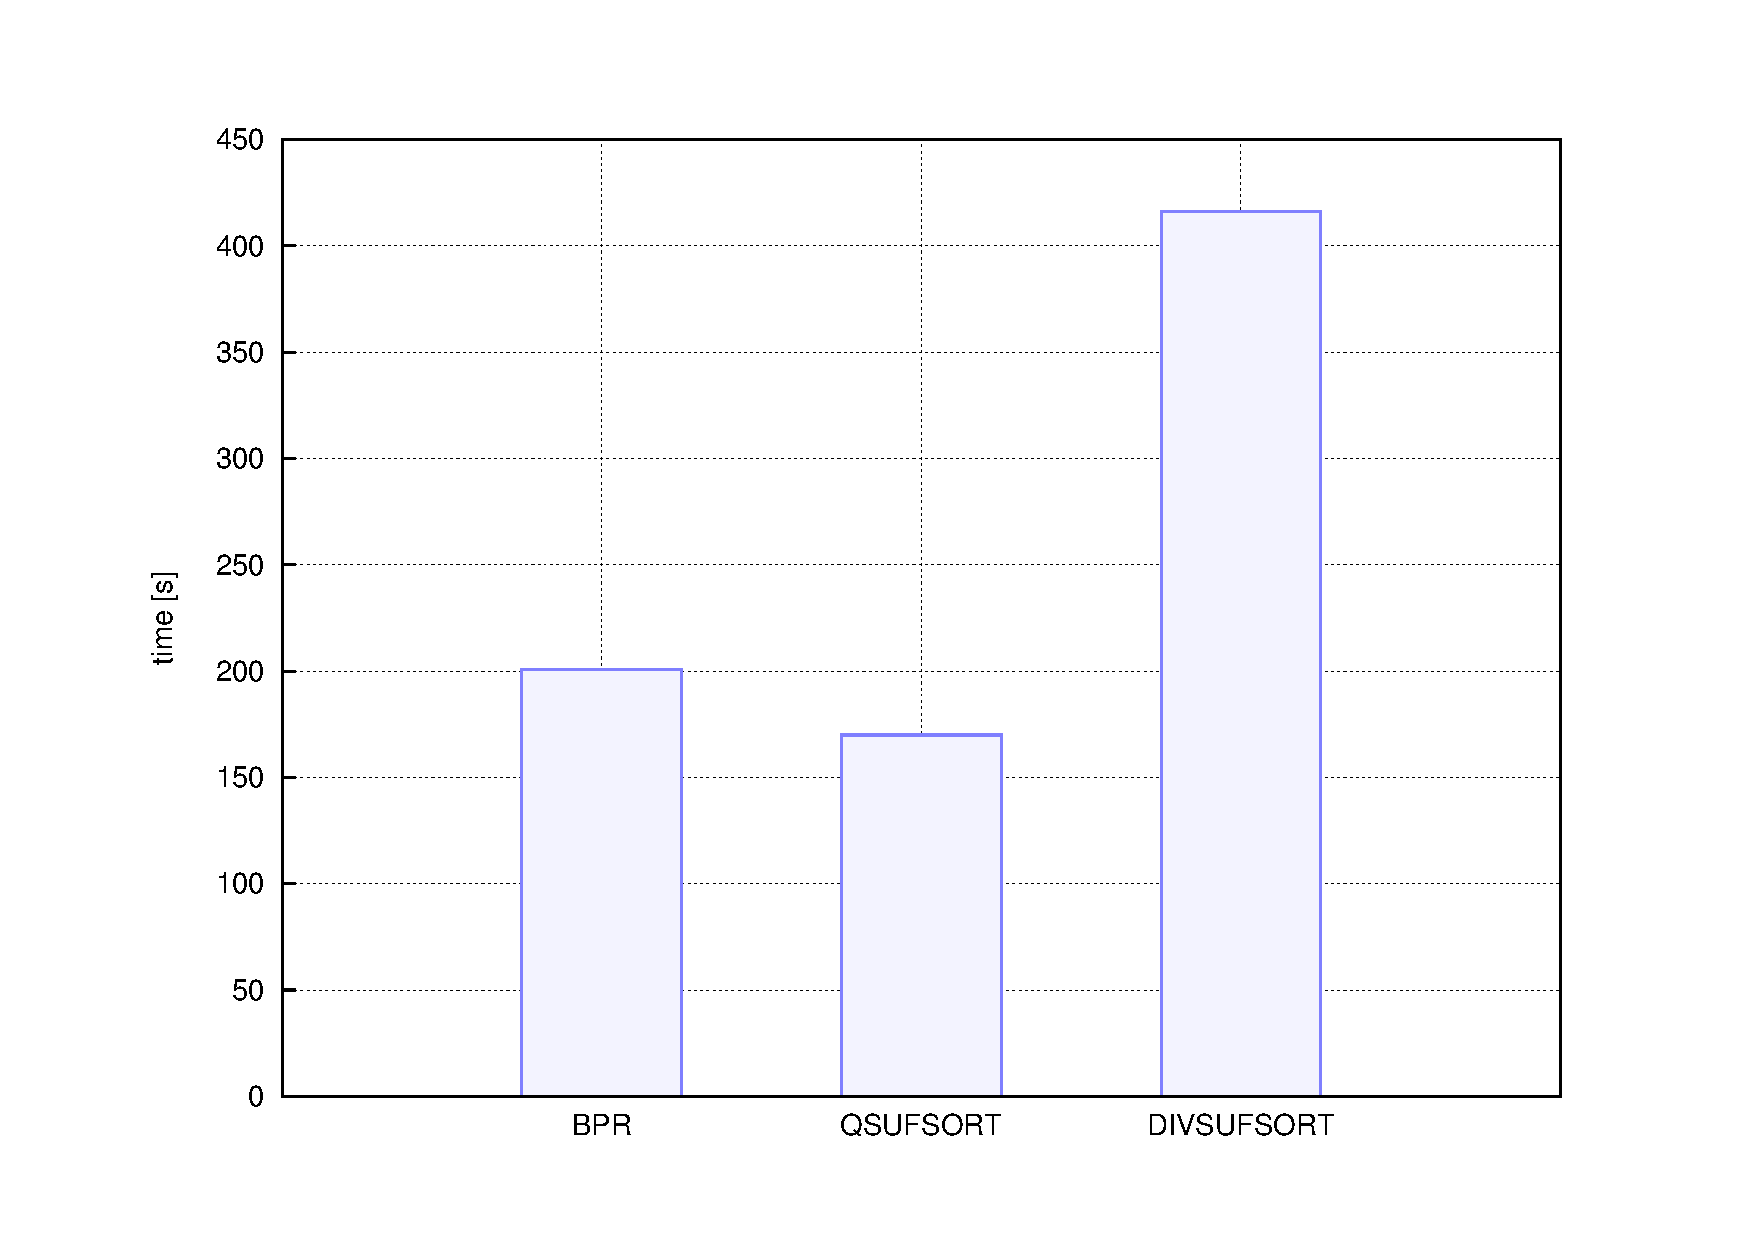
\includegraphics[width=\linewidth]{figures/results/jrockit-manzini.pdf}
        \end{center}        
	    \caption{Sumaryczny czas działania algorytmów na plikach z korpusu Giovanniego Manziniego dla maszyny wirtualnej \texttt{jrockit}.}%
    \label{rys:jrockit-manzini}
\end{figure} 


\begin{table}[p]
	\begin{center}        
 		\begin{tabular}{l r r r r } \toprule
 & \emph{bpr} & \emph{divsufsort} & \emph{qsufsort} & \emph{skew}\\ \midrule
\texttt{abac} & 1.83 & 0.05 & \textbf{0.03} & 0.06\\
\texttt{abba} & 4.41 & \textbf{2.82} & 2.85 & 11.62\\
\texttt{book1x20} & \textbf{3.85} & 4.36 & 4.24 & 23.35\\
\texttt{fib\_s14930352} & 11.77 & 6.18 & \textbf{4.15} & 15.18\\
\texttt{fss10} & 6.50 & 4.87 & \textbf{3.04} & 12.26\\
\texttt{fss9} & 1.31 & 0.80 & \textbf{0.69} & 2.32\\
\texttt{houston} & 4.05 & \textbf{0.23} & 0.53 & 1.45\\
\texttt{paper5x80} & 0.19 & 0.15 & \textbf{0.07} & 0.53\\
\texttt{test1} & 3.14 & 0.49 & \textbf{0.25} & 2.27\\
\texttt{test2} & 0.96 & 0.36 & \textbf{0.23} & 2.28\\
\texttt{test3} & 88.37 & 0.54 & \textbf{0.42} & 1.22\\
 \midrule
Total & 126.39 & 20.85 & \textbf{16.51} & 72.53\\
 \bottomrule
\end{tabular}

    \end{center}                         
	\caption{Czas działania algorytmów na plikach z korpusu \texttt{The Gauntlet} dla maszyny wirtualnej \texttt{harmony}.}%
    \label{tab:harmony-gauntlet}
\end{table}

\begin{figure}[p]
       \begin{center}
            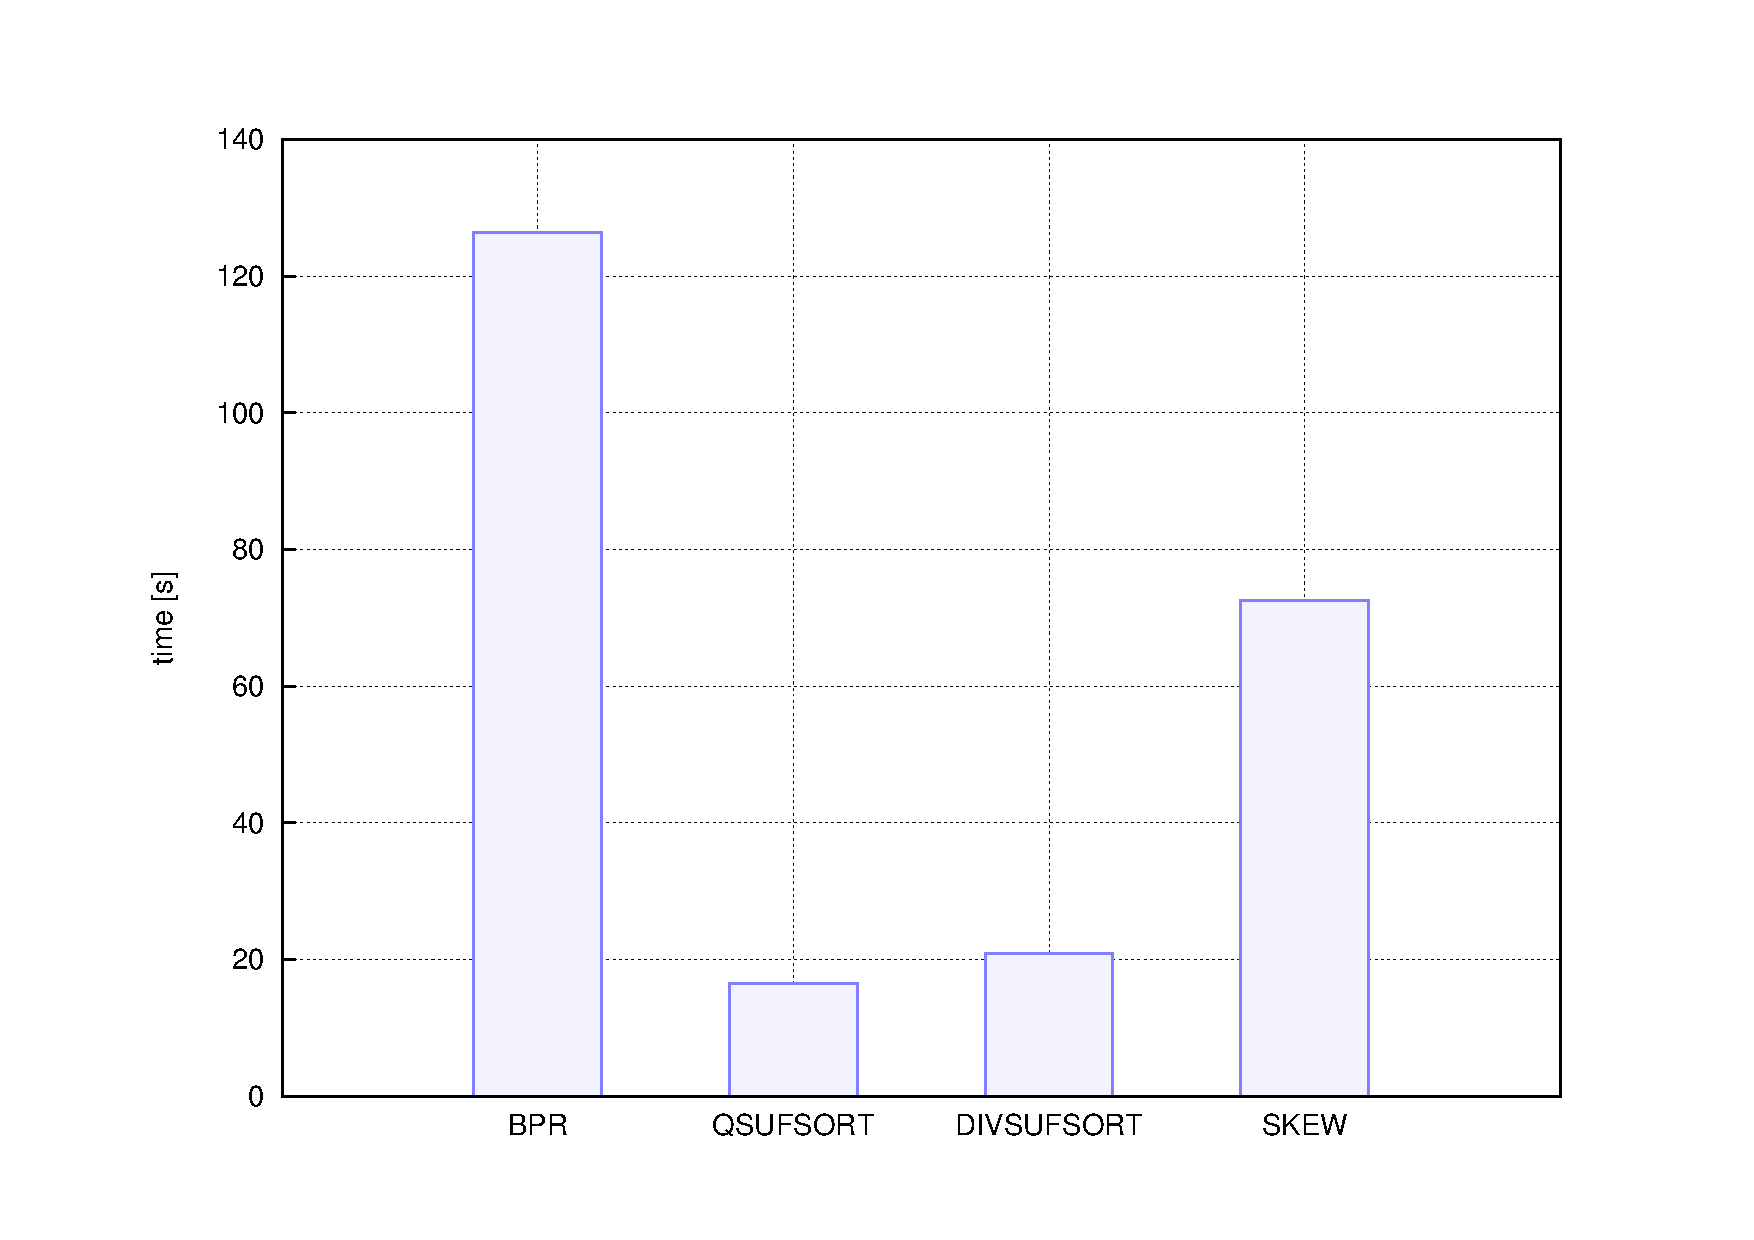
\includegraphics[width=\linewidth]{figures/results/harmony-gauntlet.pdf}
        \end{center}        
	    \caption{Sumaryczny czas działania algorytmów na plikach z korpusu \texttt{The Gauntlet} dla maszyny wirtualnej \texttt{harmony}.}%
    \label{rys:harmony-gauntlet}
\end{figure} 


\begin{table}[p]
	\begin{center}        
 		\begin{tabular}{l r r r r } \toprule
 & \emph{bpr} & \emph{divsufsort} & \emph{qsufsort} & \emph{skew}\\ \midrule
\texttt{chr22.dna} & \textbf{7.31} & 8.54 & 8.15 & 60.73\\
\texttt{etext99} & 28.21 & 29.20 & \textbf{26.35} & ---\\
\texttt{gcc-3.0.tar} & --- & 17.25 & \textbf{14.81} & ---\\
\texttt{howto} & 8.44 & 10.33 & \textbf{7.94} & 79.66\\
\texttt{jdk13c} & 16.44 & 14.74 & \textbf{12.36} & ---\\
\texttt{linux-2.4.5.tar} & 25.60 & 24.09 & \textbf{20.30} & ---\\
\texttt{rctail96} & 30.55 & 28.08 & \textbf{24.60} & ---\\
\texttt{rfc} & 28.93 & 25.92 & \textbf{24.43} & ---\\
\texttt{sprot34.dat} & 28.55 & 28.94 & \textbf{22.89} & ---\\
\texttt{w3c2} & 24.87 & 25.55 & \textbf{17.29} & ---\\
 \midrule
Total &  & 212.62 & \textbf{179.12} & \\
 \bottomrule
\end{tabular}
 
    \end{center}                         
	\caption{Czas działania algorytmów na plikach z korpusu Giovanniego Manziniego dla maszyny wirtualnej \texttt{harmony}.}%
    \label{tab:harmony-manzini}
\end{table}

\begin{figure}[p]
       \begin{center}
            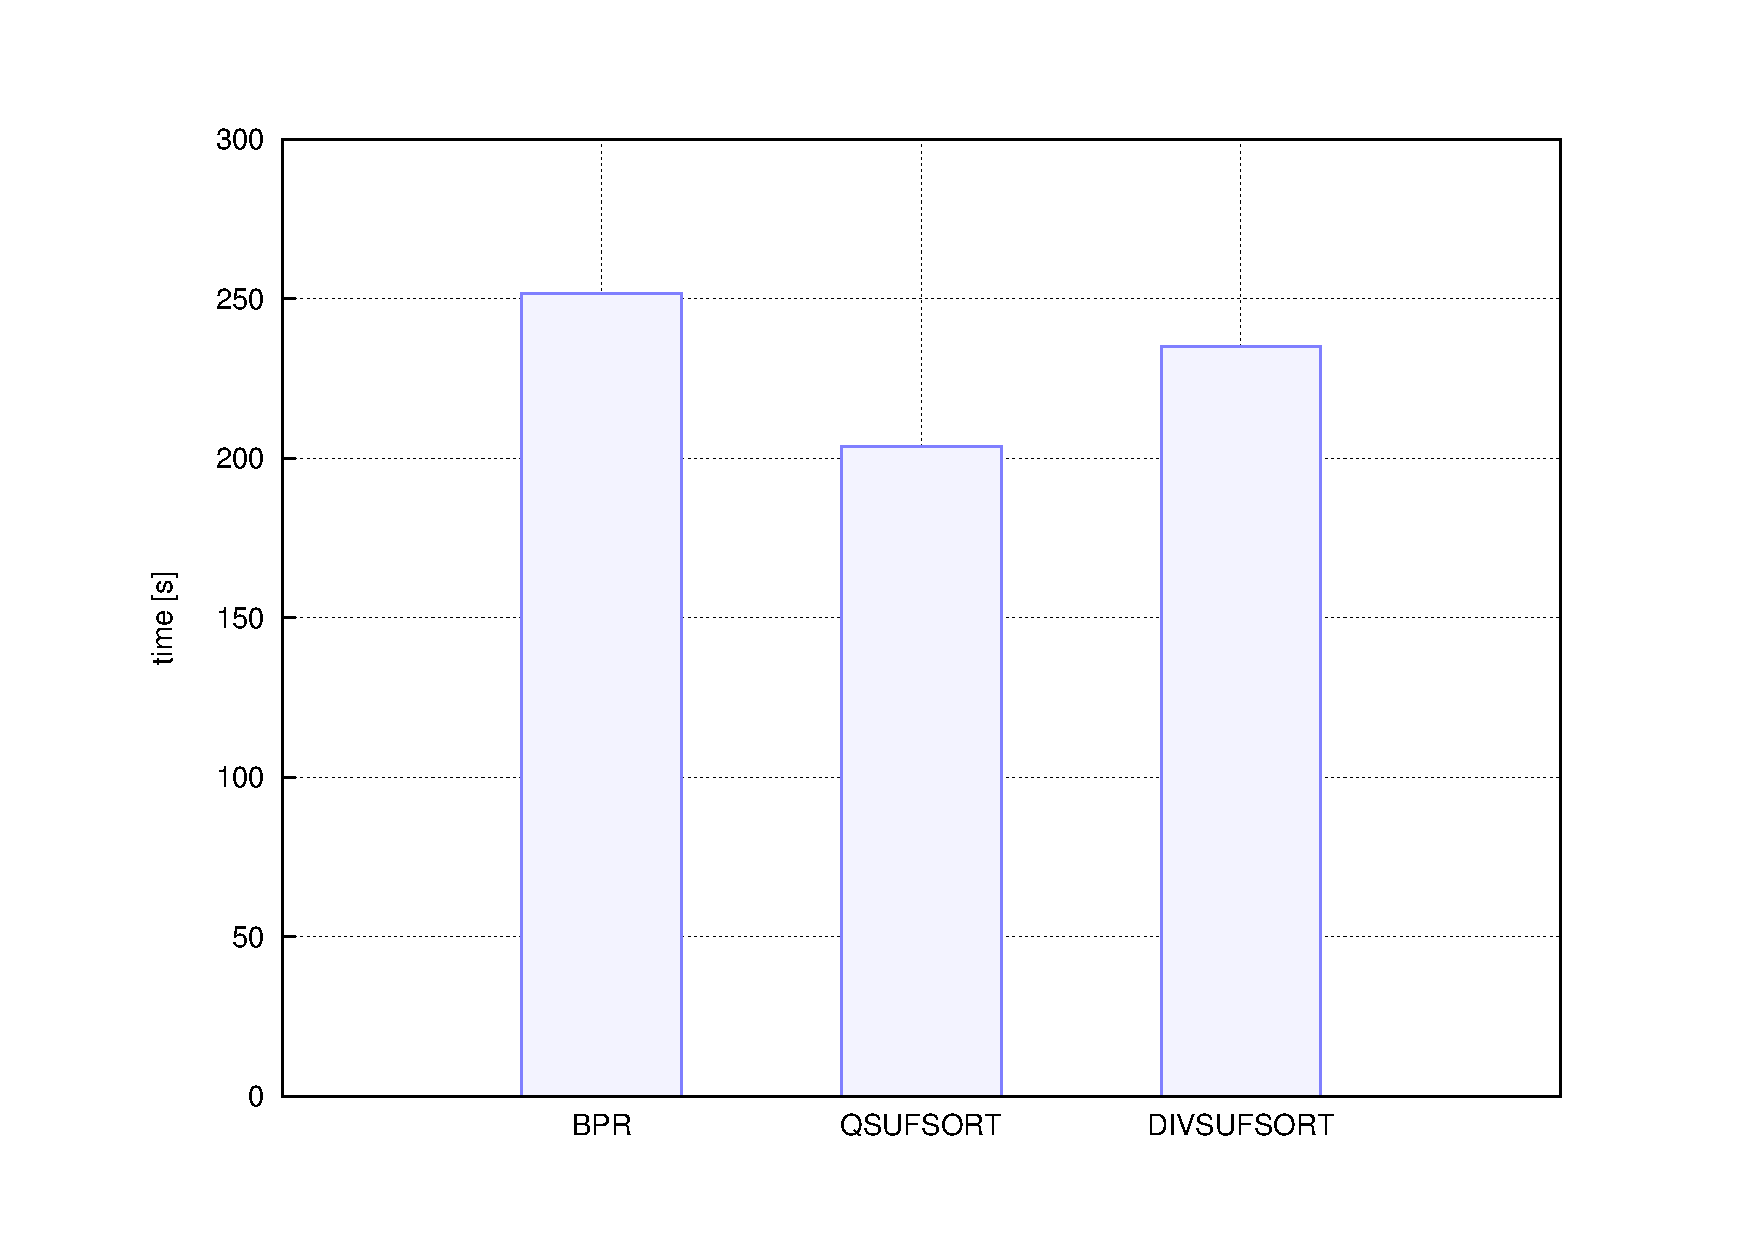
\includegraphics[width=\linewidth]{figures/results/harmony-manzini.pdf}
        \end{center}        
	    \caption{Sumaryczny czas działania algorytmów na plikach z korpusu Giovanniego Manziniego dla maszyny wirtualnej \texttt{harmony}.}%
    \label{rys:harmony-manzini}
\end{figure}
 

% Bibliography (books, articles) starts here.
\bibliographystyle{plain}{\raggedright\sloppy\small\bibliography{bibliography}}

% Web resources
\chapter*{Zasoby internetowe}\label{sect:web-resources}%
\phantomsection\addcontentsline{toc}{chapter}{Zasoby internetowe}

\newcommand{\tturl}{\begingroup \urlstyle{tt}\Url}

{\small
\begin{enumerate}[{[}A{]}]
	\item \label{hart} Project Gutenberg. \\
		\tturl{http://www.gutenberg.net}
	\item \label{aspectj} The AspectJ Project. \\
		\tturl{http://www.eclipse.org/aspectj/}
	\item \label{gauntlet}  The Gauntlet (Universal Robustness Corpus). \\
		\tturl{http://www.michael-maniscalco.com/testset/gauntlet/}
	\item \label{manzini-corpus} Manzini's Large Corpus. \\
		\tturl{http://www.mfn.unipmn.it/~manzini/lightweight/corpus/}
	% \item \label{carrot} Carrot2 Clustering Engine. \\
	% 	\tturl{http://carrot2.org/}
	% \item \label{jsa} Java Suffix Arrays. \\
	% 	\tturl{http://jsuffixarrays.org/}
	% \item \label{bsd} New BSD License \\
	% 	\tturl{http://www.opensource.org/licenses/bsd-license.php}
		
		
		\item \label{mori-benchmark} Yuta Mori, Suffix Array Construction Benchmark \\
			\tturl{http://homepage3.nifty.com/wpage/benchmark/index.html}

		\item \label{msufsort} Michael Maniscalco, The MSufSort Algorithm. \\
			\tturl{http://www.michael-maniscalco.com/msufsort.htm}

		\item \label{KScode} Peter Sanders, Skew algorithm. \\
			\tturl{http://www.mpi-inf.mpg.de/~sanders/programs/suffix/}


		\item \label{ssort}  M. Douglas McIlroy, ssort.c \\
			\tturl{http://cm.bell-labs.com/cm/who/doug/source.html}

			\item \label{archon} Dmitry A. Malyshev, Archon \\
				\tturl{http://kvgate.com/index.php?root/comp/arch/archon/}

			\item \label{MFcode} Giovanni Manzini, A Lightweight Suffix Array and BWT Construction Algorithm \\
				\tturl{http://web.unipmn.it/~manzini/lightweight/ds.tgz}
				
			\item \label{libdivsufsort} Yuta Mori, libdivsufsort project homepage. \\
				\tturl{http://code.google.com/p/libdivsufsort/}
				
				
			\item \label{LScode} N.Jesper Larsson, qsufsort.c \\
				\tturl{http://www.larsson.dogma.net/qsufsort.c}
				
\item \label{bpr-code}  Klaus-Bernd Sch\"{u}rmann i Jens Stoye, bpr downloadpage. \\
	\tturl{http://bibiserv.techfak.uni-bielefeld.de/download/tools/bpr.html}


		
\end{enumerate}
}


% Colophon is a place where you should let others know about copyrights etc.
\ppcolophon


\end{document}
